\documentclass{vldb}


\usepackage{enumitem}
\usepackage{framed}
\usepackage{cprotect}
\usepackage{enumitem}
\usepackage{listings}
\usepackage{amstext}
\usepackage{amstext}
\usepackage{pdfpages}
\usepackage{alltt}
\usepackage{epstopdf}
\usepackage{xspace,colortbl}
\usepackage[USenglish]{babel}
\usepackage{multirow}
\usepackage{url}
\usepackage{subfigure}
\usepackage{graphicx}%%
\usepackage{amssymb}
\usepackage{fmtcount}
\usepackage{amsfonts}
\usepackage{xspace}
\usepackage{amsmath}
\usepackage{multirow}
\usepackage[mathscr]{eucal}
%\usepackage{psfrag}
\usepackage{colortbl}
\usepackage{bm}
\usepackage{times}
\usepackage[nospace]{cite}
\usepackage{csquotes}

\lstset{basicstyle=\scriptsize,breaklines=true,language=SQL,belowcaptionskip=.1\baselineskip}

\linespread{0.945}

\makeatletter
\def\@copyrightspace{\relax}
\makeatother

\begin{document}

\setlength{\belowdisplayskip}{0.5pt} \setlength{\belowdisplayshortskip}{1pt}
\setlength{\abovedisplayskip}{0.5pt} \setlength{\abovedisplayshortskip}{1pt}
\setlength{\belowcaptionskip}{-10pt}
\selectfont

\newtheorem{theorem}{Theorem}
\newtheorem{example}{Example}
\newtheorem{definition}{Definition}
\newtheorem{problem}{Problem}
\newtheorem{property}{Property}
\newtheorem{proposition}{Proposition}
\newtheorem{lemma}{Lemma}
\newtheorem{corollary}{Corollary}

\newcommand{\cond}{\textrm{pred}\xspace}
\newcommand{\dataset}{data set\xspace}
\newcommand{\datasets}{data sets\xspace}
\newcommand{\spview}{\textsf{SPView}\xspace}
\newcommand{\fjview}{\textsf{FJView}\xspace}
\newcommand{\aggview}{\textsf{AggView}\xspace}
\newcommand{\hashfunc}[1]{\textsf{hash}(#1)\xspace}
\newcommand{\hashop}{\textsf{hash}\xspace}
\newcommand{\nsc}{\textsf{NormalizedSC}\xspace}
\newcommand{\rsc}{\textsf{RawSC}\xspace}

\newcommand{\avgfunc}{\ensuremath{\texttt{avg} }\xspace}
\newcommand{\maxfunc}{\ensuremath{\texttt{max} }\xspace}
\newcommand{\minfunc}{\ensuremath{\texttt{min} }\xspace}
\newcommand{\histfunc}{\ensuremath{\texttt{histogram\_numeric} }\xspace}
\newcommand{\countfunc}{\ensuremath{\texttt{count}}\xspace}
\newcommand{\sumfunc}{\ensuremath{\texttt{sum} }\xspace}
\newcommand{\varfunc}{\ensuremath{\texttt{var} }\xspace}
\newcommand{\stdfunc}{\ensuremath{\texttt{std} }\xspace}
\newcommand{\covfunc}{\ensuremath{\texttt{cov} }\xspace}
\newcommand{\corrfunc}{\ensuremath{\texttt{corr} }\xspace}
\newcommand{\medfunc}{\ensuremath{\texttt{median} }\xspace}
\newcommand{\percfunc}{\ensuremath{\texttt{percentile} }\xspace}
\newcommand{\havingfunc}{\ensuremath{\texttt{HAVING} }\xspace}
\newcommand{\selectfunc}{\ensuremath{\texttt{select} }\xspace}
\newcommand{\ratio}{\ensuremath{\rho }\xspace}


\newcommand{\insertion}{\ensuremath{\texttt{INSERT} }\xspace}
\newcommand{\update}{\ensuremath{\texttt{UPDATE} }\xspace}
\newcommand{\delete}{\ensuremath{\texttt{DELETE} }\xspace}

\newcommand{\svcfull}{Stale View Cleaning\xspace}
\newcommand{\svc}{SVC\xspace}
\newcommand{\svcnospace}{SVC}

\newcommand{\tbl}[1]{\textsf{#1}\xspace}
\newcommand{\field}[1]{\textsf{#1}\xspace}
\newcommand{\cost}{\textrm{cost}\xspace}
\newcommand{\ans}{\textsf{ans}\xspace}
\newcommand{\dans}{\Delta\textsf{ans}\xspace}
\newcommand{\cqp}{correction query processing\xspace}
\newcommand{\Cqp}{Correction query processing\xspace}

\newcommand{\reminder}[1]{{{\textcolor{magenta}{\{\{\bf #1\}\}}}\xspace}}
\newcommand{\specialcell}[2][c]{%
  \begin{tabular}[#1]{@{}c@{}}#2\end{tabular}}

\def\ojoin{\setbox0=\hbox{$\bowtie$}%
  \rule[-.02ex]{.25em}{.4pt}\llap{\rule[\ht0]{.25em}{.4pt}}}
\def\leftouterjoin{\mathbin{\ojoin\mkern-5.8mu\bowtie}}
\def\rightouterjoin{\mathbin{\bowtie\mkern-5.8mu\ojoin}}
\def\fullouterjoin{\mathbin{\ojoin\mkern-5.8mu\bowtie\mkern-5.8mu\ojoin}}

%\setlength{\belowcaptionskip}{-10pt}

%\newcommand{\reminder}[1] {}
\pagestyle{plain}

\title{Stale View Cleaning: Getting Fresh Answers from Stale Materialized Views}

\numberofauthors{1}
\author{\large Sanjay Krishnan, Jiannan Wang, Michael J. Franklin, Ken Goldberg, Tim Kraska{$\,^\dag$} \\
\vspace{.2em}\affaddr{\large UC Berkeley, ~~ $^\dag$Brown University} \\
\vspace{.1em}\affaddr{\large \{sanjaykrishnan, jnwang, franklin, goldberg\}@berkeley.edu}\\
\affaddr{\large tim\_kraska@brown.edu}
}

%\fontsize{10pt}{12pt}
%\selectfont

{\noindent \normalsize \bf Dear SIGMOD Chair and Referees: }

\vspace{.5em}

We thank the reviewers and chair for the very helpful feedback on our paper. We have addressed all of the concerns and include references to the revised text in this cover letter. 
We have significantly revised and clarified the presentation and exposition
of the paper.
To summarize the major changes:

\reminder{It would be better to add in which sections you made changes. I revised the first two points for your reference. You can revise the followings. }
\begin{enumerate}
\item Sections 1 and 2 have been revised to clarify the relationship between \sys and related work that applies active learning for data cleaning (e.g., \cite{gokhale2014corleone, DBLP:journals/pvldb/YakoutENOI11, yakout2013don}).

\item A new subsection, Section 2.1, has been added to formalize our definition of dirty data and our model for data cleaning.

\item We formalize the two subproblems addressed in this work: correctly incrementally updating a convex statistical model with newly clean data, and making data cleaning more efficient.

\item We clarified our system architecture by highlighting essential components for correctness and optional optimizations. We also present a clear overview of the data flow in \sys and which components are user-specified.

\item We have expanded our running example to clarify the key technical contributions of the paper and revised the exposition of the technical sections.

\item We included references to the related work suggested by the reviewing committee.
\end{enumerate}
Below we address each reviewer comment in detail:

\vspace{0.5em}

\subsection*{Meta Review Details} 

We would first like to clarify an important point about the subject and scope of our paper in relation to related work.
Active learning (see survey \cite{settles2010active}) is an increasingly popular technique to maximize the benefit of interactive data cleaning procedures \cite{DBLP:journals/pvldb/YakoutENOI11, gokhale2014corleone, yakout2013don, DBLP:journals/pvldb/HaasKWF015}.
In typical applications of active learning, the data cleaning algorithm is posed as a supervised learning problem (e.g., classify pairs of records as duplicates~\cite{gokhale2014corleone}) where humans iteratively label a small number of proposed fixes.
In this setting, the data cleaning is progressive in the sense that as more records are labeled, the predictive model's quality is expected to improve.
However, a key point is that this model is designed for predicting {\it clean labels} from {\it dirty} input data.  
For example, a movie recommender system may train a model on {\it dirty} movie data to deduplicate movie titles.

Our \sys setting focuses on down-stream analytic models (DSM) that expect {\it clean} input data.  
For example, a netflix recommender relies on clean movie and user preference data to predict additional user preferences.   
Certainly, data cleaning systems that employ active learning may satisfy this requirement by acquiring a set of labels, training the data cleaning model (DCM), cleaning the rest of the dataset using the DCM,
and handing the resulting dataset to the DSM.
The key limitation of this approach is that the DCM may require a very large number of labels before the DCM accuracy is sufficient for the DSM~\reminder{As we did not show this result in the experiment, probabily a more conservative way to say it is that "this approach is not aware of the down-stream analytic model when selecing a part of data to clean, thus it may waste a lot of cleaning effort in the part of the data that does not help to obtain a better analytic model at all"}.
A second limitation~\reminder{For the second limitation, I would suggest to only argue that the above approach has serious methodological problems, where you can refer reviewers to Section 2.3.}, is that if the down-stream system decided to not rely on the results of the active learning model and directly use the manually cleaned data, then
the DSM will either have high sample error due to the small number of cleaned records (assuming manual cleaning is expensive) or 
serious methodological problems if the DSM attempted to train on the combination of the cleaned and unclean data .
A final minor, but practical matter is that active learning rarely converges smoothly, and so labeling more records may not improve, and sometimes even degrade, the model quality \reminder{I would suggest to remove this minor limitation because ActiveClean seems also have this issue.}.

In contrast to the above approaches, our work {\it extends} active cleaning theory~\reminder{what is active cleaning theory?} to explicitly make use of the knowledge that the down-stream process is a machine learning model.
By doing so, we directly address the limitations above by intelligently selecting the most profitable sample of records to clean such that 
the resulting DSM will {\it provably} converge to the true, clean model, and such that we require significantly fewer data cleaning operations than the above approach \reminder{Similar as the concern that I have above, have we shown that it requires significantly fewer data cleaning operations in the experiment? }.
In addition, we generalize the active learning problem from one where only the record labels change through manual data cleaning, to one where {\it any} attribute of a record may be cleaned \reminder{I would suggest to remove it because it seems that guided data repairing can do this as well.   }.


\iffalse
Active learning is the process of prioritizing supervisor input to a machine learning model that maximizes the convergence rate.
Active learning algorithms use the current best model to acquire the most valuable future data.

In this class of use cases, active learning is used \emph{for} data cleaning, in 

% The growing popularity of predictive models in data analytics \cite{bdas, alexandrov2014stratosphere, crotty2014tupleware, hellerstein2012madlib} presents a new opportunity to apply active learning for data cleaning.

traditiona l AL is progressive in sense that more labels --> higher model quality. but these are dirty clean models!
If we use AL to clean data for downstream analytics, model wouldn't be sufficient quality, in fact, not clear what quality ought to be.
In contrast, active clean applies novel extensions to AL to generalize and apply to downstream analysitcs.

Our work contrasts in that it studies the problem of model training \emph{after} data cleaning --
specifically, given that we know that the data cleaning process (as a black box) will be used to train a down-stream model, 
how can we use that knowledge to prioritize which data is cleaned?
%In other words, this paper explores the problem of model training \emph{after} data cleaning as opposed to using a model \emph{for} data cleaning.
This problem is subtly different than active learning as currently applied in data cleaning.
Current work uses machine learning models to enhance data cleaning by predicting clean data from dirty data.
In \sys, the machine learning model is part of the data analysis, and this requires predicting clean data from \emph{clean} data.
This small change raises a number of challenges in ensuring correctness and prioritization.
\fi

\vspace{0.5em}

\noindent\noindent \textbf{M1. There should be a formal vocabulary introduced early on. The exact idea of ``dirty" here can be hard to follow: what is the exact error type(s) that the system is intended to clean?}

\vspace{0.5em}

We thank the reviewers for this important feedback and clarified that our system applies to data cleaning operations that can be modeled as record-by-record mappings between two relations with the same schema.
This model is sufficiently expressive for our experiments and a number of real-world dirty data scenarios such as attribute value canonicalization and missing value filling.
We hope to explore additional data cleaning models that include record deduplication or schema transformation in future work.
We added the following clarification to Section \ref{dmodel}:

\emph{This paper explores a model for data error where attributes of records in a relation $R$ are incorrect or missing.
Formally, the data is corrupted in a way such that there exists a supervisor (human or algorithm, in either case expensive to query), that given a dirty record can return the unique correct clean record.
Note that this does not cover errors that simultaneously affect multiple records like record deduplication or schema transformation problems.
This is modeled by a record-by-record cleaning operation $C(\cdot)$ can be applied to a record $r \in R$ to recover $r_{clean}$ \reminder{syntax error?}.
Therefore, for every $r \in R_{dirty}$ there exists a unique $r' \in R_{clean}$, and a cleaning function $C(\cdot)$, is a function that maps each $r$ to its corresponding $r'$.
We assume that there is a featurization $F(\cdot)$ which is defined over both $R_{dirty}$ and $R_{clean}$ and maps rows~\reminder{rows-> records?} to vectors in $\mathbb{R}^d$.
So each row~\reminder{row-> record?} corresponds to one training example in the predictive model.}

\vspace{0.5em}

\noindent\textbf{M2. Sections 5-7 are the technical core of the paper, and appear formal at the expense of aiding understanding. They appear to implement something that resembles active learning or bootstrapping, except inside the gradient descent loop. The motivation of some of this is not clear; is it necessary to integrate with the gradient descent? This is not how most active learning methods are implemented. Is it possible to implement these approaches in a way that is orthogonal to the SGD algorithm? The current writeup entangles some of these design choices.} 

\reminder{I think the content is there, but need to rewrite the response in a way that is more specific to the reviwer's questions. The reviwer was asking about the writing issues in Sections 5-7, but currently, they cannot easily figure out how we revise each of the sections to make our design choices more clear. Would be better to (1) add the locations of the changes in each section, and (2) say more expilictly that what design choices that we need to make and how/why we make those choices. }

Thank you for bringing this to our attention. 
In broadening interactive data cleaning to also include the downstream data analysis, the key new question is statistical validity.
\sys addresses two problems: (1) the correctness problem of how to update a dirty statistical model after data cleaning and (2) the efficiency problem of how to prioritize data cleaning based on the current best model.
In the revised text, we formalize these two problems independently (Section \ref{updp} and Section \ref{optp} respectively). 

We re-organized the paper to first describe a solution to problem (1). We argue that without an incremental optimization approach, there is a problem of model training after progressive data cleaning. Figure \ref{update-arch1} describes straight-forward applications of progressive data cleaning and model training and why these approaches have issues.
These issues can occur whether or not the data cleaning is interactive or passive, as the problem is not with the data cleaning but with the model updating procedure.
The basic problem is that given the new data the model has to be incrementally updated rather than training on a mix of dirty and clean data.
The integration with SGD is one approach to addressing problem (1).

Next, the paper describes the basic solution to problem (2). We motivate our specific choice of prioritization by describing optimality with respect to the SGD update, but we clarify the data flow and independence of these components. 
Finally, we separate optional optimizations which greatly improve the efficiency of \sys in a final technical section.

\vspace{0.5em}

\noindent\textbf{M3. In general, the distinction between an ``architecture" and an ``algorithm that fits into the architecture" is quite unclear. The problem with SGD/Active Learning above is one example.}

\reminder{Add the locations of the changes that you made for addressing this comment. }

We have revised the architecture section \reminder{(Section~?)} to highlight: user inputs, data flows in \sys, components that are essential for correctness, and components that are optimizations.
We formalize algorithmic problems~\reminder{(Section~?)} independent of the system architecture and overview the architecture in pseudocode~\reminder{(Section~?)} that describes the API for each of the components.

\reminder{Might be better to say something about the last sentence: ``The problem with SGD/Active Learning above is one example." }


\vspace{0.5em}

\noindent\textbf{M4. The paper, and especially the technical sections, would benefit enormously from a detailed running example showing how the algorithm works}

We have added a number of examples at the end of each of the technical sections. Section 4 (Architecture) ends with an intuitive end-to-end running example without technical details (Example \ref{archex}).
Section 5 (Update Problem) ends with an SVM example of how updates are propagated and calculated (Example \ref{upex}).
Section 7.1 (Detection) contains two examples for how the two different types of detectors can be used (Examples \ref{detex1} and \ref{detex2}).
Section 7.2 (Estimation) ends with an example summarizing how linearization could be applied to SVM estimation.

\vspace{0.5em}

\noindent\textbf{M5. Some connections to related work that combines machine learning and data cleaning should be made. See the other reviewers' comments.}

We highlight related work in the background section (Section \ref{alrw}):

\emph{There are a number of recent approaches that apply active learning to reduce number of records that need to be cleaned by a human.
The main idea is to treat human input as binary labels in a supervised learning problem \cite{DBLP:journals/pvldb/MozafariSFJM14}.
For example, Gokhale et al. \cite{gokhale2014corleone} applied crowdsourcing to label likely pairs of records as duplicates.
Yakout et al. \cite{DBLP:journals/pvldb/YakoutENOI11} proposed a technique called Guided Data Repair, where human input was used to confirm proposed repairs that satisfy pre-declared data quality rules.
In Gokhale et al. and Yakout et al., the goal of the learning model is to anticipate the human input and only require labels when uncertain.}

\emph{Active learning is a very powerful and general concept that goes beyond binary labels and essentially argues that not all information is created equal.
It iteratively uses the current best model to acquire the most valuable future data.
We explore how to apply this idea to analysis-driven data cleaning. 
Some data are more relevant than others to a downstream analytics, and thus, more valuable to clean.
However, the problem of prioritizing cleaning by using a user-specified downstream model is subtly different than active learning as currently applied in data cleaning.
Using machine learning to enhance data cleaning means predicting clean data from dirty data.
In \sys, machine learning is the data analysis and this requires predicting clean data from \emph{clean data}~\reminder{I did not get ``predicting clean data from \emph{clean data}".}. 
This small change~\reminder{Why is this a ``small" change?} raises a number of challenges in ensuring correctness and prioritization.}

\emph{It turns out that these two definitions are not incompatible and \sys explores a more general problem setting.
For example, rather than replacing the dirty data, corresponding clean data can be added into new columns. 
Thus, \sys can be used to train models for some learning-based data cleaning algorithms~\reminder{I did not understand that why adding new columns can imply this.}.
It can apply in a wider set of problems than existing work~\reminder{What do you mean by ``existing work"? I believe there must be many learning-based data cleaning algorithms that do not need data-quality rules or can also deal with missing values.} such as when data quality rules do not exist and numerical value imputation where human input is not binary.}

\vspace{0.5em}
In our related work section~\reminder{(Section ?)}, we highlighted the suggested references to progressive data cleaning:
\emph{When data cleaning is expensive, it is desirable to apply it \textbf{progressively}, where analysts can inspect early results with only $k \ll N$ records cleaned.
Progressive data cleaning is a well studied problem especially in the context of entity resolution \cite{altowim2014progressive, whang2014incremental, papenbrock2015progressive, gruenheid2014incremental}~\reminder{missing citation}.
Prior work has focused the problem of designing data structures and algorithms to apply data cleaning progressively.
This is challenging because many data cleaning algorithms require information from entire relations, and designing incremental models is a challenging problem even for just entity resolution.
However\reminder{Why is there a ``However"? Do you mean that progressive data cleaning is so hard, and we need to work on rule-based systems?}, over the last 5 years a number of new results have expanded progressive data cleaning to rule based systems \cite{mayfield2010eracer, DBLP:journals/pvldb/YakoutENOI11, yakout2013don}.
\sys explores the statistical implications of using progressive data cleaning before high-dimensional predictive modeling.}

\vspace{0.5em}

\emph{Recently, in works such as SampleClean \cite{wang1999sample}, the application (i.e., query workload) are used to inform data cleaning methoy~\reminder{some errors in this sentence?}.
It suffices to clean a sample of data when the data will be used to answer aggregate queries.
Sampling has also been applied to assess the number of duplicates in a relation \cite{heise2014estimating}.
When the workload is made up of aggregate queries, cleaning samples of data may suffice. 
Similarly, Bergman et al. explore the problem of query-oriented data cleaning \cite{DBLP:conf/sigmod/BergmanMNT15}. Given a query they clean data relevant to that query. }

\subsection*{Review 1 Details} 

\noindent\textbf{R1.1: At first, the problem seems a bit too specialized. The abstract is too loaded with technical terms and a turn-off. This is then mitigated in the introduction. \\
As mentioned above, the abstract is (to me) overly technical and did not make me curious. I did not know off the bat what a convex loss model is, what importance sampling is, etc.}

We revised the abstract to be more accessible:

\emph{A perennial challenge in data analytics is presence of dirty data in the form of missing, duplicate, incorrect, or inconsistent values.
Although errors can be mitigated through data cleaning, it is often very time consuming.
One approach to making data cleaning more efficient is to leverage knowledge of the downstream data analysis to prioritize those records that are most likely to affect the result.
However, data analytics increasingly consist of statistical analysis and predictive modeling which can be highly sensitive to dirty data which is only partially cleaned.
This paper explores reliable model update procedures and prioritization for progressive data cleaning.
We focus on two problems for a popular class of models called convex loss models (e.g., linear regression and SVMs): (1) the methodological problem of updating a model with partially clean data, and (2) the algorithmic problem of using information from the model to prioritize data cleaning.
The key insight of our framework is that data cleaning can be applied simultaneously with incremental optimization allowing for progressive cleaning while preserving provable properties.
Evaluation on four real-world datasets suggests that for a fixed cleaning budget, \sys returns more accurate models than uniform sampling and Active Learning when systematic corruption is sparse. }

\vspace{0.5em}

\noindent\textbf{R1.2: Poor embrace of the duplicate detection problem (see details below). Your model of the cleaner seems to preclude any duplicate detection, which certainly cannot happen on individual records. Also you extension for a set of record does not fit the problem of duplicate detection. This is in contrast, for instance, to your ER example in the second column of that page. Appendix A.1 is misleading here, as you mention with Example 7 ``in entity resolution problems..." but do not actually address that problem in the example. Fixing some common inconsistency is not entity resolution.}

We apologize for the confusing terminology and have revised our paper to clarify that we do not address record-level deduplication.
We formalized our data cleaning model to clarify this.
However, we intended to bring attention to the fact that some types of attribute level inconsistencies are addressed in similar ways to record deduplication.
For example, in our experimental dataset, the inconsistencies ``Pfizer Inc.", ``Pfizer Incorporated", and ``Pfizer" can be addressed using a blocking and matching procedure similar to that used in record deduplication but over a projection.
That said, we have removed references to entity resolution and described this in more precise terms.

\vspace{0.5em}

\noindent\textbf{R1.3: Cheated by using a narrower font than required. Will have trouble with camera ready copy if publisher insists on proper font.\\
- I would not use ``overview" as a verb...
- 3.2: the detector select -> the detector selects
- 4.3: Wrong quotation marks around ``learning".
- QED symbols on page 8 are ugly when placed directly after formula. 
- References need a clean up. Just as an example: Venue is missing for [24], year is mentioned 3 times for [8], [11], etc. Page numbers appear sporadically.}

We have addressed all of the formatting and copy editing issues.

\vspace{0.5em}

\noindent\textbf{R1.4:There is some related work specifically addressing progressive/incremental entity resolution. You might want to point your readers to this.
\\E.g.
\\- Incremental entity resolution on rules and data, Whang et al. VLDB Journal 2014
\\- Progressive duplicate detection, Papenbrock et al., TKDE 2015
\\- Incremental record linkage, Gruenheid et al., PVLDB 2014
\\- Another work that is related is ``Estimating the Number and Sizes of Fuzzy-Duplicate Clusters" by Heise et al. CIKM 2014, which also incrementally cleans samples of data to predict in this case the number of record matches.}

Thank you for highlighting these references, and we have included them in our related work~\reminder{(Section?)}.

\vspace{0.5em}

\noindent\textbf{- Page 1, last paragraph in column 1 reads as if reference to [3] is a reaction to the work referenced in the previous sentence, i.e., the term ``remains" is misleading.
- I did not quite understand the short paragraph on crowd-sourcing. Why is this even relevant?
 I believe it would suffice to simply state that cleansing is expensive...}

We appreciate the thorough feedback and have tightened up the writing in the introduction. In particular, we have consolidated the motivation to a single paragraph describing the expense of data cleaning.


\subsection*{Review 2 Details}

\noindent\textbf{R2.1: The definition of ``clean data" is imprecise and not clear. It appears that ``cleaning" in this system refers to entity resolution, cleaning w.r.t. dependencies, and possibly other actions as needed by the application. This makes it difficult to gauge overall accuracy when there are different interpretations of cleanliness. It is not clear how entity resolution and cleaning w.r.t. dependencies can be done holistically.}

As mentioned above~\reminder{``above" is a vague word. Need a conrete location.}, we have included a formalizing of the data cleaning models addressed in this paper in Section 2.1. 

\vspace{0.5em}

\noindent\textbf{R2.2: The paper describes a problem setting focused on modelling the iterative cleaning process rather than actual data management problems. The paper may be better suited at an ML venue.}

We have revised the paper~\reminder{where?} to emphasize its relevance to a database audience. We argue that the straight-forward application of existing progressive data cleaning methods, which have been widely proposed in the community, can lead to error-prone and misleading results if used in conjunction with predictive modeling. 

\vspace{0.5em}

\noindent\textbf{R2.3: Missing references to related work on interactive data cleaning. For the comparative evaluation, 2/3 techniques are ML based techniques, not interactive data cleaning systems. See D2.\\
D2: Data cleaning systems have also considered interactive engagement with the user and the application of ML techniques. 
i) Mohamed Yakout, Laure Berti-Equille, Ahmed K. Elmagarmid. Don't be SCAREd: use SCalable Automatic REpairing with maximal likelihood and bounded changes. SIGMOD Conference 2013: 553-564
ii) Mohamed Yakout, Ahmed K. Elmagarmid, Jennifer Neville, Mourad Ouzzani, Ihab F. Ilyas.
Guided data repair. PVLDB 4(5): 279-289 (2011).
}

We thank the reviewer for these references and have clarified the key differences with our work. \reminder{This short answer will not work for this important question. We need to explain in detail the difference of ActiveClean from existing interative data-cleaning systems. }

\vspace{0.5em}

\textbf{R2.4: Sampling is an important part of the framework and influences the accuracy of the cleaning. Yet, there is little discussion on sampling rate, or how a sample is chosen.}

We revised Sections 6 and 7 to be more precise about the sampling.
Section 6 describes sampling without estimation or detection:

\emph{The model update received a sample with probabilities $p(\cdot)$.
\sys uses a sampling algorithm that selects the most valuable records to clean with higher probability. }

\vspace{0.5em}

Section 7 describes how sampling can be improved with estimation and detection and intuition on why those optimizations improve result accuracy.

\vspace{0.5em}

\textbf{R2.5: An end-to-end running example in Section 5 is needed to highlight the intuition of the cleaning process.}

We have added a number of examples to describe the intuition for each of the technical sections. \reminder{We should not assume that each reviewer will read meta reviews. It would be better to point them to the right place. For example, you can ask the reviewer to see M4 for more detail. }

\vspace{0.5em}


\subsection*{Review 3 Details}
\noindent\textbf{R3.1: The authors do not distinguish between the system architecture and the individual issues that they are presenting.}

\reminder{Say how you address this issue in meta reviews. Otherwise, the reviewer will miss that.}

As mentioned earlier we now distinguish between the correctness problem and the efficiency problem.
We have revised to emphasize that \sys is one implementation of algorithms that address this problem.

\vspace{0.5em}

\noindent\textbf{R3.2: The paper uses lots of definitions, and a multitude of that do not necessarily contribute to readability.
Without being an expert in the field, I found it extremely difficult to follow the paper as it touches upon multiple problems at the same time: data cleaning, model training, convex analytics, etc., uses definitions, notation and lots of examples that did not allow me to have a global understanding of the work.\\
I would prefer to have a more focused paper on one of these aspects that has concrete goals and then, having an overview of the architecture of the system as a small section. I believe that the architecture should not be the focus and the skeleton of this paper. Instead, I believe that the authors could focus on the individual problems.}

\reminder{(1). We actually did a lot of work to reorganize the paper, rewrite the paper, add new stuffs to the paper, etc to make the paper more readable and more focused. But it's hard to tell from the current response. Maybe we can list all the changes that we made for the sake of readability and being more focused.}

\reminder{(2). Ask the reviewer to see M2 and M3 for his/her concerns about the architecture/algorithm relationship, and design goals.}

We have revised the paper to improve readability. In particular, we have consolidated a number of sections~\reminder{``a number of sections" sound vague} and moved non-essential equations to the appendix. We do however believe that data cleaning needs to be understood as an essential part of the model training process. Data analysis is increasingly using predictive models and these models are highly sensitive to data cleaning procedures.


\setcounter{page}{1}

\maketitle

\iffalse

\begin{abstract}
Materialized views, stored pre-computed query results, are used to facilitate queries on large datasets.
Materialized views can become out-date when base tables change and queries will give \emph{stale} results.
Maintaining materialized views has been well studied but is often very costly.
In this work, we model the view maintenance problem as a data cleaning problem and treat out-of-date rows materialized views as a type of data error.
In particular, we analyze the maintenance procedure for the views and infer how these updates affect a queries on a the stale view.
For common aggregate queries (\sumfunc, \countfunc, and \avgfunc), we can derive a correction factor from the sample to ``clean" the stale query result.
We bound our corrections in analytic confidence intervals, and in fact, we show that our technique is optimal with respect to estimate variance.
As sampling can be sensitive to long-tailed distributions, we further consider an outlier indexing technique to give increased accuracy when the data distributions are skewed.
We evaluate this approach on real and synthetic datasets and in both a single node (MySQL) and distributed environment (Apache Spark).
In one large scale experiment using 20-node Apache Spark cluster, we derived a 700,000,000 row view from a 1TB activity log base dataset.
We found that maintaining a 5\% sample was 16.3x faster than full maintenance yet only with mean query error of 1.2\%.
\end{abstract}
\fi

\vspace{-1em}

\begin{abstract}
Materialized views (MVs), stored pre-computed results, are widely used to facilitate fast queries on large datasets. When new records arrive at a high rate, it is infeasible to continuously update (maintain) MVs and a common solution is to defer maintenance by batching updates together. Between batches the MVs become increasingly stale with incorrect, missing, and superfluous rows leading to increasingly inaccurate query results.
We propose \svcfull (\svc) which addresses this problem from a data cleaning perspective. 
%We take inspiration from recent results in data cleaning which combine sampling and cleaning for accurate query processing. 
In \svc, we efficiently clean a sample of rows from a stale MV, and use the clean sample to estimate aggregate query results.
While approximate, the estimated query results reflect the most recent data.
As sampling can be sensitive to long-tailed distributions, we further explore an outlier indexing technique to give increased accuracy when the data distributions are skewed. \svc complements existing deferred maintenance approaches by giving accurate and bounded query answers between maintenance. We evaluate our method on a real dataset of workloads from the TPC-D benchmark and a real video distribution application.  Our experiments confirm our theoretical results: (1) cleaning an MV sample is more efficient than full view maintenance, (2) the estimated results are more accurate than using the stale MV, and (3) \svc is applicable for a wide variety of MVs.
\end{abstract}


% !TEX root = demo.tex
\section{Introduction}\label{sec:intro}

\begin{figure}[t]
\centering
\vspace{-0.5cm}
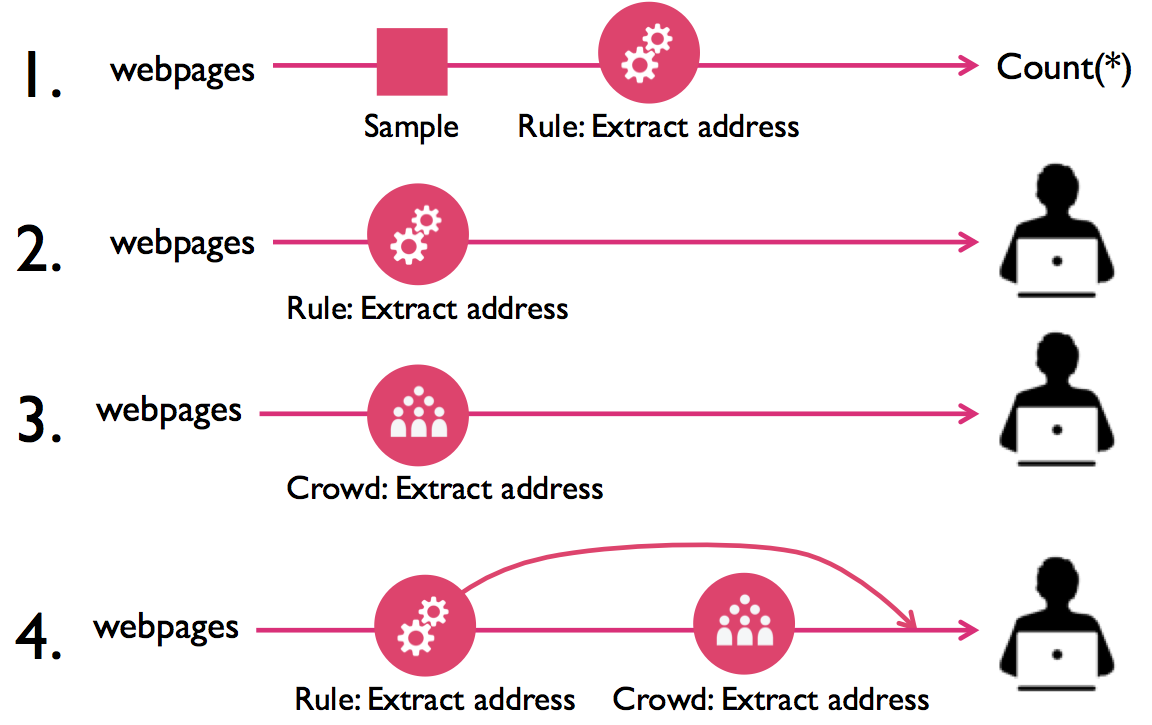
\includegraphics[width = .4\textwidth]{figs/lifecycle.png}
\vspace{-0.4cm}
\caption{Example iterations on the design of the portion of a cleaning plan that extracts restaurant addresses from their unstructured webpages.  
1) An exploratory plan that uses a sample to evaluate a simple address extraction method.
2) A plan that applies the method to the entire dataset. The quality is unsatisfactory. 
3) An alternate plan that uses manual crowd extraction. The quality is now high, but the crowd-based extractor is slow. 
4) A hybrid plan that sends only difficult webpages to the crowd, maximizing accuracy without sacrificing latency.}
\label{fig:ex-plan}
\vspace{-0.3cm}
\end{figure}
% why feedback loops exist/are important (cite Joe’s shit in the past 3 years, blinkdb, etc.). highlight domain specificity. Large variety of data cleaning tasks

%
% General comment that data cleaning is important:
%
The ease of acquiring and merging many large-scale data sources has led to a prevalence of dirty data.
Unfortunately, blindly using results that are derived from dirty data can lead to hidden yet significant errors in modern data-driven applications, so data must be cleaned before it is used.
But because data cleaning is often specific to the domain, dataset, and eventual analysis, analysts report spending upwards of 80\% of their time on problems in data cleaning~\cite{kandel2012}.
The analyst is faced with a breadth of possible errors that are manifest in the data and a variety of options to resolve them.
She must go through the cleaning process via trial and error, deciding for each of her data sources what to extract, how to clean it, and whether that cleaning will significantly change results.

Data cleaning is inherently iterative and Figure~\ref{fig:ex-plan} shows a common progression for the development of a data cleaning plan, in this case the extraction of a restaurant's address from its unstructured webpage.
While this operation can easily be represented at a \textit{logical} level by its input and output schema, there is a huge space of possible \textit{physical} implementations of the logical operators. 
For example, extraction could depend on manually specified rules (\textit{rule-based}), use models trained on previously extracted ground truth records (\textit{learning-based}), ask crowd workers to extract the desired data fields (\textit{crowd-based}), or some combination of the three (e.g., active learning, which uses crowd workers to provide labels for a learning-based approach).
Even after selecting (say) a crowd-based operator, many parameters might influence the quality of the output data or the speed and cost of cleaning: the number of crowd workers who vote on the extraction for a given webpage, the amount each worker is paid, etc.
A priori, a data analyst has little intuition for what physical plan will be optimal in this large space.

Note that in the evolution of the data cleaning plan in Figure~\ref{fig:ex-plan}, our data analyst needed to make many decisions manually about the choice of physical operators by reasoning about their latency, accuracy, and cost. 
Making the wrong decision, for example using the crowd when it only marginally improves accuracy, can be very costly.
A general, scalable, and interactive system that supports rapid iteration on candidate plans would greatly aid this process.

%The prevalance of data cleaning systems in both the research and industrial communities --
%Corleone does blah, XXX addresses blah. Nadeef does blah -- speak to the importance of a
%data cleaning framework as part of the modern big data ecosystems. \ewu{include open access of data in argument?} \jn{We also need to take a look at data cleaning systems in industry. }


% why existing systems suck aka related work
% 1. have slow feedback loops (dataset-dependence, …)
% 2. solve very specific data-cleaning tasks
%Since the beginning of data management, systems have been explored by both the research and industrial communities to improve data cleaning efficiency and quality.
Existing systems seldom address the end-to-end iterative data cleaning process described above.
Extract-transform-load (ETL) systems~\cite{informatica,talend,apachefalcon} require developers to manually write data cleaning rules and execute them as long batch jobs, 
and constraint-driven tools allow analysts to define ``data quality rules" and automatically propose corrections to maximally satisfy these rules \cite{DBLP:conf/sigmod/DallachiesaEEEIOT13}.
Unfortunately, neither provide the opportunity for iteration or user feedback, inhibiting the user's ability to rapidly prototype different data cleaning solutions.
Projects such as Wrangler~\cite{wrangler,trifacta} and OpenRefine~\cite{openrefine} support iteration with spreadsheet-style interfaces that enable the user to compose data cleaning sequences by directly manipulating a sample of the data and applying these sequences to the full dataset.
However, they are limited to specific cleaning tasks such as simple text transformations, do not support crowd-based processing at scale, and cannot incorporate user feedback to optimize the physical implementation of the data cleaning sequences.
Crowd-based~\cite{gokhale2014corleone,stonebraker2013data} systems have been proposed to relieve the data analyst of the burden of rule specification or manual cleaning, but are usually specific to a single cleaning task (e.g.,~\cite{gokhale2014corleone,park2014crowdfill,eracer,chen2014integrating}), preventing end-to-end optimization of the entire cleaning plan.
These existing limitations suggest the need for a system that is general enough to adapt to a wide range of data cleaning applications, scales to large datasets, and natively supports fast-feedback interactions to enable rapid data cleaning iteration.

In this paper, we introduce \sys, a system designed to support the iterative development and optimization of data cleaning plans end to end.
\sys allows users to specify declarative data cleaning plans composed of rule-based, learning-based, or crowd-based operators, then iterate rapidly on plans with cost-aware recommendations for improving the accuracy or latency of a plan.
The effects of a plan can be viewed early using sampling and approximate query processing techniques~\cite{wang1999sample}.

Supporting these capabilities requires a combination of careful engineering 
as well as tackling several research challenges:

\squishlist
\item \textbf{Sampling}: We provide sampling as a first-class logical operator for data cleaning plans that tolerate approximation, and use it to speed up iteration on early-stage plans.

\item \textbf{Recommendation}: We recommend cost-aware changes to in-flight cleaning plans that allow users to trade off accuracy and latency, and provide efficient mechanisms for implementing recommended changes without re-executing the plan on already cleaned tuples.

\item \textbf{Crowd Latency}: We leverage techniques for straggler mitigation~\cite{venkataraman2014power} and model crowd worker speed and accuracy to reduce the (often rate-limiting) latency of crowd data cleaning, consistently retrieving results in seconds rather than hours.
\squishend

In our demonstration, we will run an entity resolution plan on two restaurant datasets, and
show how \sys can be used to 1) specify, modify, and execute a data cleaning plan,
2) quickly clean a sample to characterize how a plan is performing, and
3) observe the same cleaning plans running on multiple datasets.
Users can execute plans over a live crowd that uses the audience as workers, or a simulated crowd
that uses pre-collected crowd responses. The dashboard (Figure~\ref{screenshot}) also provides a live inspection
interface to view the status of the cleaning plan as it executes.

\vspace{-0.2cm}
%Our contributions/requirements
%different ways to tighten the feedback loop:
%end-to-end latency/cost (operator optimization)
%looking versus touching
%Adding introspection (more points of observation)
%hot-swapping (more points of changing plans)
%We have built an end-to-end data cleaning framework with these requirements in mind. (... things we do …) (... engineering contributions …).
%In this demonstration, we highlight the benefits of improving feedback loops for data cleaning using X datasets by optimizing a data cleaning pipeline for one data set/cleaning task, then quickly fitting the pipeline to another dataset.


\if{0}

\jn{Honestly, I didn't quite buy declarativity of the system. In my opinion, data cleaning is so domain specific. It's hard to make it declarative. For a given domain, people may need to write their own data cleaning system. There is a lack of a data cleaning framework that they can build based on. This motivates us to develop such framework. 


We analyze a large variety of domain specific data cleaning systems, and identify several key components: declarative data cleaning operators (e.g., similarity joins), active learning, and crowd/expert sourcing platforms that they require. In our framework, we abstract these components, and implement them in a general way. 

We mainly address two challenges: extensibility and scalability. For the former one, we came up with a nice data-cleaning pipeline API, which people can easily use to compose their own data cleaning tasks. For the latter one, we address it in two aspects: Sampling + Asynchrony.}

\ewu{That's fair, will need to address why a framework is necessary and what benefits it provides.  I think a framework is the correct pitch, hard to sell a set of operators.  Are the above challenges -- extensibility and scalability -- actually difficult?  Worried it's straightforward application of existing techniques.}



In contrast, our work is based on the observation that the majority of data cleaning workflows
can be decomposed into a small set of logical operations (in addition to traditional database operators):
filter based on constraints, extract new fields from existing data, and a similarity join to match
similar or duplicate records. \ewu{quickly validate why this observation holds.} \jn{Yes! I also found that Sec 2.3 has more operators than you describe here.}  
By designing a system around these core operators, we can provide a vast library of physical  
data cleaning operators that span the range of algorithmic, machine learning, and human computation-based
implementations that are necessary practical data cleaning pipelines.   \ewu{Describe live inspection as 
a core feature or is it too easy?}

Designing such a system requires tackling several design challenges:

\begin{enumerate}
\item Speed
\item Quality
\item API Design/extensibilty
\end{enumerate}



We have implemented an initial version of \sys on top of the AMPLab Spark stack, which provides us 
with access to its advanced distributed processing and machine learning features.  Our goal for the current
version is to implement the core mechanisms for declarative specification of the
data cleaning pipeline, solidify the API design, and incle support for, and implementations of,
multiple classes of physical data cleaning operators.


\fi



\if{0}

Cleaning, pre-processing, and formatting data is a required first step in any data analytics pipeline.
However, despite this importance, large-scale data analytics platforms such as Spark or Hadoop lack integrated data cleaning frameworks.
There are a few challenges in building a general purpose data cleaning framework: (1) data cleaning is often
domain specific and requires specialized software targeted at one or a handful of data sources \cite{wang1999sample}, (2) data cleaning is often 
expensive as it increasingly involves human effort via crowdsourcing or experts \cite{DBLP:conf/sigmod/GokhaleDDNRSZ14}, and (3) learning how to clean dirty data from examples
is often hard without a greatly restricted set of operators \cite{DBLP:conf/uist/GuoKHH11}.

We address this problem in \projx by designing a Spark library of composable and scalable data cleaning primitives.
\projx abstracts the logical data cleaning operators: Extraction, Similarity Join, Filtering, from the physical implementation i.e, Rule, Crowd, or Machine Learning.
We interface these primitives through a DSL with which a user can build data cleaning operators that suit their needs.
\projx provides transparent optimizations for each of the components and their composition.
In this demonstration proposal, we present \projx and highlight some of its key features.
While there are many existing systems that do one aspect of data cleaning and transformation (e.g Entity Resolution or Extraction), 
many real world data cleaning tasks have multiple types of errors.
Composing disparate systems can lead to complex code and inefficiencies at scale.
With \projx, we hope to design a set of optimized composable primitives that span a large space of data cleaning tasks.

The first key feature of \projx is that it provides optimized distributed implementations 
of the physical data cleaning operators.
For example, a key step in many deduplication algorithms is a Similarity Join which finds all pairs of records that are within some similarity threshold.
A naive implementation of a Similarity Join would apply a similarity function to all pairs of records.
However, in \projx, we provide optimized implementations of certain common similarity functions (e.g Jaccard, Edit Distance, etc.) that allow for 
a combined broadcast join and prefix filtering which intelligently skips pairs of records using a broadcasted inverted index.

Another feature of \projx is managing the latency and the scale problems of crowd-based data cleaning. 
Crowdsourcing is increasingly prevalent in data cleaning, and \projx provides physical crowd-based implementations
of the logical operators.
However, crowds work at a different latency and scale point in comparison to distributed analytics platforms.
To address the latency problem, we build asychrony into the system.
The user can query intermediate results at any time as crowd responses stream in.
To address the scale issue, \projx provides sampling primitives.
The glue that ties all of the crowd components together is a Machine Learning technique called Active Learning.
As we collect more and more crowd responses, we learn a model that predicts these responses to apply it on the uncleaned data.
Active Learning selects the most informative questions to ask the crowd.

Finally, \projx provides an approximate query processing (AQP) framework.
With slow asynchronous data cleaning algorithms as in crowdsourcing, we need 
to define clear semantics for the intermediate results.
Our AQP framework uses the algorithms proposed in \cite{wang1999sample}, to estimate and bound early results.
It is also common for data scientists to prototype expensive data cleaning pipelines on samples and AQP allows quick evaluation of
aggregate query results on a cleaned sample.

\subsection{Demonstration Scenario}
\reminder{TODO}

\fi




\if{0}
Consider for example, the ability to rapidly understand the types of errors that are present, as well as prevalance of 
these errors is cruicial.



Before an organization can use a new dataset as part of their analysis pipeline
(e.g., to build complex learning models or answer analyst queries)
the errors in the dataset need to be removed in order to ensure accurate conclusions.  

Modern data-driven organizations rely on the ability to ingest and generate large data sets from 
disparate sources, and combine the data together to build complex models or answer analytical questions.  
For example, a restaurant review website may collect restaurant listings by scraping data from webpages or purchasing them from external sources, and
restaurant visitation information for sources such as OpenTable or FourSquare, and aggregate the data to
model user eating habits.  
The set of cleaning tasks necessary for each of these data sources is highly domain and application specific,
and oftentimes the developer is concurrently trying to clean the data source as well as understand its properties.


Oftentimes, these data sources have data quality issues that require a complex data cleaning pipeline -- 
e.g., data extraction, re-formatting, identification and fixes of missing or incorrect values,
and removal of redundant information -- before the data is useable by downstream processes.
Data sources are often domain specific and new for the data analyst, 
As datasets continue to grow, and organizations make use of mure and more datasets, the ability to
rapidly clean the data is more important.  
\fi

\section{Problem Formalization}
This section formalizes the problem addressed in the paper.

\subsection{Convex Models}
This work focuses on an initial class of well analyzed predictive analytics problems; ones that can be expressed as the minimization of convex loss functions.
Convex loss minimization problems are amenable a variety of incremental optimization methodologies with provable guarantees (see Friedman, Hastie, and Tibshirani \cite{friedman2001elements} for an introduction).
Examples includes all generalized linear models (including linear and logistic regression), all variants of support vector machines, and in fact, means and medians are also special cases. 

Formally, for labeled training examples $\{(x_{i},y_{i})\}_{i=1}^{N}$, the problem is to find a vector of \emph{model parameters} $\theta$ by minimizing a loss function $\phi$ over all training examples:
\[
 \theta^{*}=\arg\min_{\theta}\sum_{i=1}^{N}\phi(x_{i},y_{i},\theta)
\]
Where $\phi$ is a convex function in $\theta$.
For example, in a linear regression $\phi$ is:
\[
\phi(x_{i},y_{i},\theta) = \|\theta^Tx_{i} - y_i \|_2^2
\]
Typically, a \emph{regularization} term $r(\theta)$ is added to this problem.
$r(\theta)$ penalizes high or low values of feature weights in $\theta$ to avoid overfitting to noise in the training examples.
\[
 \theta^{*}=\arg\min_{\theta}\sum_{i=1}^{N}\phi(x_{i},y_{i},\theta) + r(\theta)
\]
In this work, without loss of generality, we will include the regularization as part of the loss function i.e., $\phi(x_{i},y_{i},\theta)$ includes $r(\theta)$.

\subsection{Problem 1. Correct Update Problem}\label{updp}
Let $R_{dirty} \subseteq R$ be the subset of records that are dirty, and $S$ be a sample (possibly non-uniform but with known probabilities) of the records $R_{dirty}$.
\sys applies the user specified cleaning function $C(\cdot)$ to the sample:
\[
S_{clean} = C(S)
\]
Given newly cleaned data $S_{clean}$ and a dirty model $\theta^{(d)}$, the model update problem is to calculate $\theta^{new}$. 
$\theta^{new}$ will have some error between with respect to the true model $\theta^{(c)}$ (if the entire dataset is cleaned):
\[
error(\theta^{new}) = \| \theta^{new} - \theta^{(c)} \|
\]
We call the update algorithm ``reliable" if the expected error is upper bounded by a monotonically decreasing function $f$ of the amount of cleaned data:
\[
\mathbb{E}(error(\theta^{new})) = O(f(\mid S_{clean} \mid))
\]
and is also upper bounded by a monotonically increasing function of the initial error:
\[
\mathbb{E}(error(\theta^{new})) = O(g(\| \theta^{(d)} - \theta^{(c)} \|))
\]
Intuitively, reliable means that more cleaning and less initial error should imply more accuracy; avoiding the pitfalls of dimensionality and Simpson's paradox.

\vspace{0.5em}

\emph{The Correct Update Problem is to reliably update the model $\theta^{(d)}$ with a sample of cleaned data.}

\subsection{Problem 2. Efficiency Problem}\label{optp}
The efficiency problem is to select $S_{clean}$ such that the expected error $\mathbb{E}(error(\theta^{new}))$ is minimized.
\sys uses previously cleaned data to estimate the value of data cleaning on new records.
Then it draws a sample of records $S_{dirty} \subseteq R_{dirty}$. This is a non-uniform sample where each record $r$ has a sampling probability $p(r)$ based on the estimates.
We derive the optimal sampling distribution for the SGD updates, and show how the theoretical optimal can be approximated.

\vspace{0.5em}

\emph{The Efficiency Problem is to select a sampling distribution $p(\cdot)$ over all records such that the expected error w.r.t to the model if trained on fully clean data is minimized.}

\subsection{Metrics}
There are two standard metrics that we will use to measure the performance of \sys:

\vspace{0.25em}

\noindent\textbf{Model Error. } Let $\theta$ be the model trained with \sys, and let $\theta^*$ be the model trained on the same data if all of the records were cleaned. Then the model error is defined as $\|\theta - \theta^*\|$.

\vspace{0.25em}

\noindent\textbf{Testing Error. } Let $\theta$ be the model trained with \sys, and let $\theta^*$ be the model trained on the same data if all of the records were cleaned. Let $T(\theta)$ be the out-of-sample testing error when the dirty model is applied to the clean data, and $T(\theta^*)$ be the test error when the clean model is applied to the clean data. The testing error is defined as $T(\theta) - T(\theta^*)$





\iffalse
\subsection{\sys Problem}
The core problem addressed by \sys is incremental model update while progressively cleaning data.

\begin{problem}[ActiveClean Problem]\label{activeclean}\sloppy
Let $R$ be a dirty relation, $F(r) \mapsto (x,y)$ be a featurization that maps
a record $r \in R$ to a feature vector $x$ and label $y$, $\phi$ be a convex regularized loss,
and $C(r) \mapsto r_{clean}$ be a cleaning technique that maps a record to its cleaned value. 
Given these inputs, the \sys problem is to return a \textbf{reliable} estimate $\hat{\theta}$ of the clean model for any limit $k$ on the number of times the data cleaning $C(\cdot)$ can be applied.

\vspace{0.5em}

\textbf{Reliable} precisely means that the expected error in this estimate (i.e., L2 difference w.r.t a model trained on a fully cleaned dataset) is bounded above by a monotonic function in $k$ and a monotonic function of the error in the dirty model.
\end{problem}
\fi


\iffalse
From a systems perspective, data cleaning and model training happen at very different time scales.
When humans are involved, per record latencies for data cleaning are orders of magnitude larger than the CPU time needed for model training.
We can compare recent results in data cleaning to a model training framework like CoCoA implemented on Spark \cite{jaggi2014communication}.
Per record, BigDansing, a highly optimized automated Spark-based data cleaning system is 15.5x slower than CoCoA\footnote{For CoCoA to reach a precision of 1e-3}.
Crowd based techniques like CrowdFill \cite{park2014crowdfill} and CrowdER \cite{wang2012crowder} are over 100,000x slower per record. 
Consequently, all of the optimizations in \sys are designed to address data cleaning latency (i.e., more progress with fewer cleaned records) rather than optimizing for numerical computation (i.e., process fewer records).
\fi



\iffalse
Here is an example application of \sys with our running example:
\begin{example}
The analyst first trains her SVM model on the dirty data ignoring the effects of the errors returning a model $\theta^{(d)}$.
She decides that she has a budget of cleaning $100$ records, and decides to clean the 100 records in batches of 10 (set based on how fast she can clean the data, and how often she wants to see an updated result).
She initializes \sys with $\theta^{(d)}$.
\sys samples an initial batch of 10 records.
She manually cleans those records by merging similar drug names, making corporation names consistent, and fixing incorrect labels.
After each batch, the model is updated with the most recent cleaning results $\theta^{(t)}$.
The model improves after each iteration.
After $t=10$ of cleaning, the analyst has an accurate model trained with 100 cleaned records but still utilizes the entire dirty data.
\end{example}



\subsection{Two perspectives on error}
When faced with such errors there are two contrasting perspectives from the Machine Learning and the Database communities.

\vspace{0.5em}

\noindent\textbf{Existing Database Literature. } 
Traditionally, cleaning is agnostic to the queries and analysis that happens downstream. 
This perspective breaks down when cleaning is so expensive that we can only clean a small number of records.
Ideally, we should clean the records that are most valuable to the downstream analysis.

\vspace{0.5em}

\noindent\textbf{Existing  Machine Learning Literature. } The Machine Learning community has focused on
designing models that are robust to outliers (i.e., values far away from the typical value)
For example, in the case of linear regression, we can change the $L_2$ norm to an $L_1$ norm to mitigate the effect of outliers:
\[
\phi(x_{i}^T\theta,y_{i}) = \|\theta^Tx_{i} - y_i \|_1
\]
The quadratic L2 loss implies that examples that deviate far from the typical example are quadratically penalized as opposed to linearly penalized with the L1 loss.
There is a natural tradeoff between robustness and efficiency.
The more robust a technique is, the less efficient it will be (i.e., estimate variance for a fixed number of training examples).
Robust techniques are best suited for random errors that look significantly different the rest of the examples.
When errors are systematic, the Machine Learning answer has been to design features in such a way that they are robust to some systematic bias.
For example, in image processing, scale-invariant feature transforms (SIFT) are widely applied that allow for image models invariant to pose or scaling issues.

\vspace{0.5em}

\noindent\textbf{The \sys Contribution. } We try to bring two perspectives together in this work to address the problem of expensive to clean systematic errors, namely the Database idea of data cleaning and the Machine Learning formalization of empirical risk minimization.
Some errors require expensive cleaning procedures, increasingly using the crowd, and we joint have a time budget on cleaning and analysis.
\sys prioritizes cleaning with respect to an estimated impact on the clean model.



\subsection{SampleClean Project}

Traditionally, data cleaning has explored expensive, up-front cleaning of entire datasets for increased query accuracy.
We proposed the SampleClean problem, in which an analyst cleans a small sample of data, and then estimates the result to an aggregate query e.g., \sumfunc, \countfunc, or \avgfunc.
The main insight from the SampleClean project is that highly accurate answers for aggregate queries does not require cleaning the full dataset.
Generalizing this insight, there is a deep relationship between the application (i.e., the query) and how an analyst should budget their effort in data cleaning.
In fact, \avgfunc and \sumfunc queries are a special case of the convex loss minimization discussed in the previous section:
\[
\phi = (x_{i} - \theta)^2
\]

We then extended the SampleClean work to study cleaning Materialized Views \cite{technicalReport}.
Suppose base data is updated with insertions, deletions, or updates, we explored how we could efficiently propagate
changes to a sample of the view instead of the full view.
Subsequent queries on the view could be answered approximate.

The SampleClean problem inspired an eponymous system that implements sampling, data cleaning, and approximate query processing on the Apache Spark stack \cite{sampleclean}.
Also included in the Apache Spark stack are Machine Learning libraries including MLlib \cite{mllib} and GraphX \cite{graphx}.
The in-memory architecture of the Apache Spark stack allows for increasingly interactive analysis \cite{AgarwalMPMMS13, armbrust2015spark}.
Analysts can prototype data processing workflows on samples to evaluate performance before running expensive batch processing jobs on entire datasets.
With data cleaning and machine learning libraries in the same software ecosystem, we see a new opportunity for joint optimization for interactive model building.



\subsection{Stochastic Gradient Descent}
Sampling is a natural part of any Machine Learning workflow, as stochastic optimization is widely used to fit model parameters.
The problems described in the previous subsections are often trained using a technique called Stochastic Gradient Descent (SGD) or one of its variants.
The basic idea of SGD is to draw a data point at random, calculate the gradient at that point, and then update a current best estimate with that gradient.
\[
\theta^{(t+1)}\leftarrow\theta^{(t)}-\gamma\nabla\phi(x_{i}^T\theta,y_{i})
\]
 SGD can also be applied in a ``mini-batch" mode, where we draw a subset of data $S^{(t)}$ at random and update with the average gradient.
 \[
 \theta^{(t+1)}\leftarrow\theta^{(t)}-\frac{\gamma}{\|S^{(t)}\|}\sum_{i\in S^{(t)}}\nabla\phi(x_{i}^T\theta,y_{i})
 \]

We can use this workflow for designing an anytime data cleaning methodology.
As data is sampled, we can clean the samples.
The analyst then can stop at anytime and use the best model at that instant.
SGD and its variants are well-studied and there are lower-bounds on the convergence rates using these techniques. 
Recently, a number of works have explored non-uniform sampling distributions for stochastic optimization \cite{zhao2014stochastic, qu2014randomized}.
The main insight is that non-uniform distributions may on average estimate the gradient accurately.
In this work, we explore how to design such a non-uniform distribution for iterative data cleaning.

\fi


 

\vspace{-1em}
\section{Framework Overview}\label{sec-arch}
In this section, we formalize the two main problems that \svc addresses: (1) cleaning the staleness errors in a sample of a MV and (2) answering an aggregate query with a clean sample.

\subsection{Notation and Definitions}\label{notation}
In \svc, we explore the problem of approximate aggregate query processing on stale materialized views using a data cleaning approach.
We assume that these materialized views are periodically maintained and thus are stale in between maintenance periods.
The focus of this paper is analytic workloads where the typical query is a group by aggregate on relatively large views.
\svc provides a framework for increased query accuracy for a flexible additional maintenance cost that can scale with system constraints.

%\reminder{You have defined $\mathcal{D}$, $\{R_i\}$, etc in Definition 1. Maybe you can move Def 1 to this Section?}
\noindent \textbf{Materialized View:} Let $\mathcal{D}$ be a database which is a collection of relations $\{R_i\}$. A \emph{materialized view} $S$ is the result of applying a \emph{view definition} to $\mathcal{D}$. 
View definitions are composed of standard relational algebra expressions: Select ($\sigma_{\phi}$), Project ($\Pi$), Join ($\bowtie$), Aggregation ($\gamma$), Union ($\cup$), Intersection ($\cap$) and Difference ($-$). 
We use the following parametrized notation for joins, aggregations and generalized projections:
\begin{itemize}[noitemsep] \sloppy
	\item $\Pi_{a_1,a_2,...,a_k}(R)$: Generalized projection selects attributes $\{a_1,a_2,...,a_k\}$ from $R$, allowing for new columns that are arithmetic transformations of attributes (e.g., $a_1+a_2$).
	\item $\bowtie_{\phi (r1,r2)}(R_1,R_2)$: Join selects all tuples in $R_1 \times R_2$ that satisfy $\phi (r_1,r_2)$. We use $\bowtie$ to denote all types of joins even extended outer joins such as $\rightouterjoin,\leftouterjoin,\fullouterjoin$.
	\item $\gamma_{f,A}(R)$: Apply the aggregate function $f$ to the relation R grouped by the distinct values of $A$, where $A$ is a subset of the attributes.  
	The DISTINCT operation can be considered as a special case of the Aggregation operation. 
\end{itemize}
The composition of the unary and binary relational expressions can be represented as a tree, which is called the \emph{expression tree}.
At the leaves of the tree are all of the \emph{base relations} for a view.
Each node of the tree is the result of applying one of the above relational expressions to a relation.
To avoid ambiguity, we refer to tuples of the base relations as \emph{records} and tuples of derived relations as \emph{rows}.

\noindent \textbf{Primary Key: } We assume that each of the base relations has a \emph{primary key}. If this is not the case, we can always add an extra column 
that assigns an increasing sequence of integers to each record.
For the defined relational expressions, every row in a materialized view can be also be given a primary key \cite{DBLP:journals/vldb/CuiW03, DBLP:conf/sigmod/ZengGMZ14},
which we will describe in Section \ref{sampling}. 
This primary key is formally a subset of attributes $u \subseteq \{a_1,a_2,...,a_k\}$ such that all $s \in S(u)$ are unique.
We denote the entire row for that primary key as a selection $\sigma_u(S)$.

\vspace{.25em}

\noindent \textbf{Staleness: } For each relation $R_i$ there is a set of insertions $\Delta R_i$ (modeled as a relation)
and a set of deletions $\nabla R_i$.
An ``update'' to $R_i$ can be modeled as a deletion and then an insertion.
We refer to the set of insertion and deletion relations as ``delta relations" denoted by $\partial \mathcal{D}$:
\[
	\partial \mathcal{D} = \{\Delta R_1,...,\Delta R_k\} \cup \{\nabla R_1,...,\nabla R_k\}
\]
A view $S$ is considered \emph{stale} when there exist insertions or deletions to any of its base relations.
This means that at least one of the delta relations in $\partial \mathcal{D}$ is non-empty.

\vspace{.25em}

\noindent \textbf{Maintenance: } There may be multiple ways (e.g., incremental maintenance or recomputation) to maintain a view $S$, and we denote the up-to-date view as $S'$.
We formalize the procedure to maintain the view as a \emph{maintenance strategy} $\mathcal{M}$.
A maintenance strategy is a relational expression the execution of which will return $S'$.
It is a function of the database $\mathcal{D}$, the stale view $S$, and all the insertion and deletion relations $\partial \mathcal{D}$. 
In this work, we consider maintenance strategies composed of the same relational expressions as materialized views described above.
\[
S' = \mathcal{M}(S,\mathcal{D}, \partial D)
\]

\vspace{.25em}

\noindent \textbf{Staleness as Data Error: } The consequences of staleness are incorrect, missing, and superfluous rows. 
Formally, for a stale view $S$ with primary key $u$ and an up-to-date view $S'$:
\begin{itemize}[noitemsep] \sloppy
	\item \textbf{Incorrect: } Incorrect row errors are the set of rows (identified by the primary key) that are updated in $S'$: \[\{\forall u \in S : (\exists u \in S' \wedge (\sigma_u(S) \ne \sigma_u(S')))\}\]
	\item \textbf{Missing: } Missing row errors are the set of rows (identified by the primary key) that exist in the up-to-date view but not in the stale view: \[\{\forall u \in S' : \not \exists u \in S\}\]
	\item \textbf{Superfluous: } Superfluous row errors are the set of rows (identified by the primary key) that exist in the stale view but not in the up-to-date view : \[\{ \forall u \in S : \not\exists u \in S' \}\]
\end{itemize}

\vspace{.25em}

\iffalse
\begin{figure}[t] \vspace{-2em}
\centering
 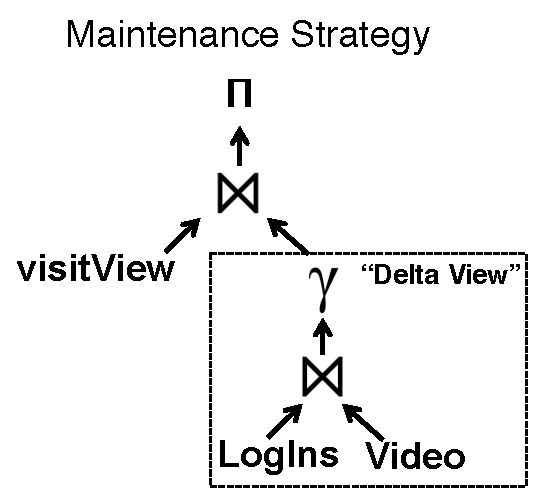
\includegraphics[scale=0.32]{figs/example_expression_tree.pdf} \vspace{-.5em}
 \caption{\reminder{(1). the view definition is different from the one in Sec 2.1; (2) Even if they are the same, it seems not necessary to show it again; (3) Right now you have (b) to show maintenance strategy; maybe you can replace (a) with a figure that shows primary key and ``staleness ad data error"} For our example, we represent the expression tree of the maintenance strategy. We first calculate a delta view using the new insertions and then join this view with the old view.\label{exexpr}}\vspace{-1.5em}
\end{figure}

\vspace{0.45em}
\fi

\noindent \textbf{Uniform Random Sampling: }
We define a sampling ratio $m\in [0,1]$ and for each row in a view $S$, we include it into a sample with probability $m$.
We use the ``hat'' notation (e.g., $\widehat{S}$) to denote sampled relations and sampled relational expressions.
We say the relation $\widehat{S}$ is a \emph{uniform sample} of $S$ if
\[\text{(1) } \forall s \in \widehat{S} : s \in S\text{;~~~~~ (2) }Pr(s_1 \in \widehat{S}) =  Pr(s_2 \in \widehat{S}) = m\]
We say a sample is \emph{clean} if an only if it is a uniform random sample of the up-to-date view $S'$. 

\vspace{0.25em}

\begin{example}\label{concepts}
In this example, we summarize all of the key concepts and terminology pertaining to materialized views, stale data error, and maintenance strategies.
Our example view, visitView, joins the Log table with the Video table and counts the visits for each video grouped by videoId.
Since there is a foreign key relationship between the relations, this is just a visit count for each unique video with additional attributes. 
The primary keys of the base relations are: sessionId for Log and videoId for Video.

If new records have been added to the Log table the visitView is considered stale.
Incorrect rows in the view are videos for which the visitCount is incorrect and missing rows are videos that had not yet been viewed once at the time of materialization. 
While not possible in our running example, superfluous rows would be videos whose Log records have all been deleted.
Formally, in this example our database is $\mathcal{D}=(Video, Log)$, and the delta relations are $\partial\mathcal{D}=(LogIns)$. 

Suppose, we apply the change-table IVM algorithm proposed in \cite{gupta1995maintenance}:
\vspace{-.55em}
\begin{enumerate}[noitemsep]
\item Create a ``delta view" by applying the view definition to LogIns. That is, calculate the visit count per video on the new logs:
\[
 \gamma(Video \bowtie LogIns)
\]
\item Take the full outer join of the ``delta view" with the stale view visitView (equality on videoId).
\[
 VisitView \fullouterjoin \gamma(Video \bowtie LogIns)
\]
\item Apply the generalized projection operator to add the visitCount in the delta view to each of the rows in visitView where we treat a NULL value as 0: 
\[
 \Pi (VisitView \fullouterjoin \gamma(Video \bowtie LogIns))
\]
Therefore, the maintenance strategy is:
\[
 \mathcal{M}(\{VisitView\},\{Video, Log\}, \{LogIns\})
\]
\[
\text{\hspace{0.7em}} = \Pi (VisitView \fullouterjoin \gamma(Video \bowtie LogIns))
\]
\end{enumerate}

\end{example}

%\begin{figure}[t] \vspace{-2em}
%\centering
% 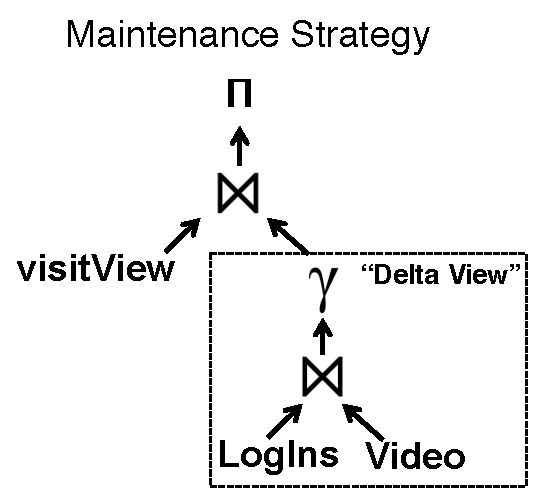
\includegraphics[scale=0.35]{figs/example_expression_tree.pdf} \vspace{-.5em}
% \caption{We illustrate the maintenance strategy of our example view, visitView, in an expression tree. \label{maintstrat}}\vspace{-1.75em}
%\end{figure}

%While, uniform sampling supports a wide variety of query types, it may have issues with queries with highly selective predicates.
%Stratfied sampling has been proposed to mitigate this problem as in the BlinkDB project \cite{AgarwalMPMMS13}.
%However, this requires that we know our query workload in advance.  
%In this paper, we do not discuss stratified sampling and will explore this further in future work.

\subsection{\svc Workflow}
%We summarize the system in Figure \ref{sys-arch} in our introduction.
In this section, we first present an overview of the \svc workflow, and then formalize two challenging problems that we address in the workflow. Formally, the workflow of \svc is:
\begin{enumerate}[noitemsep]
\item We are given a view $S$.
\item $\mathcal{M}$ defines the maintenance strategy that updates $S$ at each maintenance period.
\item The view $S$ is stale between periodic maintenance, and the up-to-date view should be $S'$.
\item \emph{(Problem 1: Stale Sample View Cleaning)} We find an expression $\mathcal{C}$ derived from $\mathcal{M}$ 
that cleans a uniform random sample of the stale view $\widehat{S}$ to produce a ``clean" sample of the up-to-date
view $\widehat{S'}$.
\item \emph{(Problem 2. Query Result Estimation)} Given an aggregate query $q$and the state query result $q(S)$, we use $\widehat{S'}$ and $\widehat{S}$ to estimate the up-to-date result.
\item We optionally maintain an index of outliers $o$ for improved estimation in skewed data.
\end{enumerate} 

\noindent\textbf{Stale Sample View Cleaning: }
The first problem addressed in this paper is how to clean a sample of the stale materialized view.
\begin{problem}[Stale Sample View Cleaning]
We are given a stale view $S$, a sample of this stale view $\widehat{S}$ with ratio $m$, the maintenance strategy $\mathcal{M}$, the base relations $\mathcal{D}$, and
the insertion and deletion relations $\partial \mathcal{D}$.
We want to find a relational expression $\mathcal{C}$ such that:
\[
\widehat{S}' = \mathcal{C}(\widehat{S},\mathcal{D},\partial \mathcal{D})
\]
Where $\widehat{S}'$ is a sample of the up-to-date view with ratio $m$. 
\end{problem}

\noindent\textbf{Query Result Estimation: }
The second problem addressed in this paper is query result estimation.
\begin{problem}[Query Result Estimation]
Let $q$ be an aggregate query of the following form \footnote{\scriptsize For simplicity, we exclude the group by clause for all queries in the paper, as it can be modeled as part of the \textsf{Condition}.}:
\begin{lstlisting} [mathescape,basicstyle={\scriptsize}]
SELECT $agg(a)$ FROM View WHERE Condition(A);
\end{lstlisting}
If the view $S$ is stale, then the result will be incorrect by some value~$c$:
\[
q(S') = q(S) + c
\]
Our objective is to find an estimator $f$ such that:
\[
q(S') \approx f(q(S),\widehat{S},\widehat{S}')
\] 
\end{problem}

\begin{example}\label{infexample}
Suppose a user wants to know how many videos have received more than 100 views.
\begin{lstlisting}[basicstyle={\scriptsize}]
SELECT COUNT(1) FROM visitView WHERE visitCount > 100;
\end{lstlisting}
Let us suppose the user runs the query and result is $45$.
However, there have now been new records inserted into the Log table making this result stale (for clarity no changes to \tbl{Video} or deletions).
First, we take a sample of \tbl{visitView} and suppose this sample is a 5\% sample.

In Stale Sample View Cleaning (Problem 1), we calculate an expression $\mathcal{C}$ based on the maintenance strategy $\mathcal{M}$ described in Example \ref{concepts},
takes the database $\mathcal{D}$ (\tbl{Log} and \tbl{Video}), and the delta relation $\partial \mathcal{D}$ (\tbl{LogIns}).
$\mathcal{C}$ is an optimized relational expression that materializes only a sample of of the updates.
In Query Result Estimation (Problem 2), we take the result of running $\mathcal{C}$ and estimate our above query.
\end{example}

\iffalse
Our query correction component takes the two corresponding samples $\widehat{S'}$ and $\widehat{S}$, and calculates a correction to~$q(S)$.

Like similar restrictions in other sample-based systems \cite{agarwalknowing}, there are restrictions on the queries $q$ on the view that we can answer. 
In the SampleClean work, we focused on \sumfunc, \countfunc, and \avgfunc queries of the form\footnote{\scriptsize For simplicity, we exclude the group by clause for all queries in the paper, as it can be modeled as part of the \textsf{Condition}.}: 
\begin{lstlisting} [mathescape,basicstyle={\scriptsize}]
SELECT $f(a)$ FROM View WHERE Condition(A);
\end{lstlisting}
In this work, we expand the scope of the query processing, and consider general non-nested aggregate queries with predicates.

We also consider correcting stale non-nested select queries of the following form with predicates:
\begin{lstlisting} [mathescape,basicstyle={\scriptsize}]
SELECT * FROM View WHERE Condition(A);
\end{lstlisting}
As with all sample estimates, the accuracy increases with sample size, thus less selective predicates lead to more accurate results.




Note, that this definition is slightly different from the reservoir sampling techniques studied in AQP \cite{DBLP:journals/toms/Vitter85} which find a uniform sample of fixed \emph{size} $k\le \mid S \mid$.
Our sampling ratio gives a sample of the size $k$ in expectation, however, the actual size from any given instance may be slightly different.
For large sample sizes, there is little difference between the techniques since the actual size of using a sample ratio will be close to $k$.
The uniform sample model represents our algorithm which uses hashing better and also makes the presentation of our analysis more clear.

Furthermore, any ``black-box'' uniform sampling algorithm can be used to achieve a reservoir sample.
The use of one technique over another does not affect the general principles or the statistics of \svc, only the 
notation in the analysis.


%\vspace{2em}
\subsection{Problem Statements}
\subsubsection{View Maintenance as Data Cleaning}\label{cleaning}
%In \svc, we model staleness in an MV as a type of data error.
We formalize the problem of correcting staleness as a data cleaning operation so we can apply our data cleaning approach.
In the unsampled case, $\mathcal{M}$ defines a data cleaning operation.
If we are given a materialized view $S$ and we know the base relations have had insertions and deletions, then there are three possible types of error:
(1) a row in $S$ needs to be updated, (2) a row in $S$ needs to be deleted, and (3) new row needs to be inserted into $S$.
Applying $\mathcal{M}$ removes these errors making the view ``clean".
%In the absence of these errors, we call a view \emph{up-to-date}.

However, now suppose we have a sampled view $\widehat{S}$, simply applying updates to the rows in the sample may not suffice.
If new rows need to be inserted into $S$, those will never be represented in the sample violating our uniform sampling.
Thus, we define cleaning in the following way: suppose we have a stale uniform sample $\widehat{S}$, cleaning this sample
should give us $\widehat{S'}$ a uniform sample of the up-to-date view $S'$ with the same sampling ratio.
Formally, this can be represented as the following operations: (1) if an update is needed, update the row, (2) if a row needs to be deleted, delete the row, and (3) for all new rows that need to be inserted into the view $S$ insert a random sample of ratio $m$.

Due to the insertions, the defined data cleaning on a sample does not necessarily give a unique $\widehat{S'}$, so the next question is how to formalize the link between $\widehat{S}$ and $\widehat{S'}$. 
To link a corresponding stale sample (dirty data) and up-to-date sample (clean data), we define the following property:
\begin{definition}[Correspondence]
$\widehat{S'}$ and $\widehat{S}$ are uniform samples of $S'$ and $S$, respectively.  We say $\widehat{S'}$ and $\widehat{S}$ correspond if and only if:
\vspace{-.25em}
\begin{itemize}[noitemsep]
\item For every row $r$ in $\widehat{S}$ that required a delete, $r \not\in \widehat{S'}$
\item For every row $r$ in $\widehat{S}$ that required an update to $r'$, $r' \in \widehat{S'}$
\item For every row $r$ in $\widehat{S}$  that was unchanged, $r \in \widehat{S'}$
\item For every row $r$ in $S$ but not in $\widehat{S}$, $r \not\in \widehat{S'}$
\end{itemize}
\vspace{-.25em}
%\item For every row $r$ in $S'$ that is newly inserted, $r \not\in \widehat{S}$.
%\item If a row $r$ requires an update and then a deletion. The deletion takes precedence and $r \not\in \widehat{S'}$.
%\item Rows that are inserted trivially satisfy the conditions since those rows are not contained in $S$ or $\widehat{S}$.
\label{correspondence}
\end{definition}
%This definition of correspondence gives us a way to get two samples from which we can take a row-by-row difference.
%There is some nuance in how to handle null values which we discuss in Section \ref{correction}.

The goal of \svc is to efficiently produce a corresponding up-to-date sample from a stale one thus cleaning the sample.
In the first component of \svc (Section \ref{sampling}), we take as input a uniform sample of a stale view $\widehat{S}$, a maintenance strategy $\mathcal{M}$, and a set of updates $\{\Delta R_i\} \cup \{\nabla R_i\}$.
We return $\widehat{S'}$, a clean uniform sample (a uniform sample of $S'$) that satisfies the correspondence property with $\widehat{S}$.

\iffalse

\begin{example}[Correspondence]
Suppose \tbl{countView} has 4 video rows: 
\begin{lstlisting} [mathescape]
V1 (visitCount = 4), V2 (visitCount = 6), V3 (visitCount = 1), V4 (visitCount = 1)
\end{lstlisting}
We take a sample of \tbl{countView} and call it \tbl{countViewSample} that contains V1 and V2.
\tbl{LogIns} has new logs of 1 visit for V1 and 1 visit for a new video V5.
An up-to-date sample that corresponds is:
\begin{lstlisting} [mathescape]
V1 (visitCount = 4+1), V2 (visitCount = 6)
\end{lstlisting}
An up-to-date sample that does \emph{not} corresponds is: 
\begin{lstlisting} [mathescape]
V1 (visitCount = 4+1), V3 (visitCount = 1)
\end{lstlisting}
This is because V2 was unchanged and therefore should be included in the sample.
\end{example}
\fi

\subsubsection{Query Result Correction}
In the query result correction phase, we take a query result on a stale view and use the up-to-date sample to compensate for the staleness.
Given a query $q$ which has been applied to the stale view $q(S)$ giving a stale result.
Our query correction component takes the two corresponding samples $\widehat{S'}$ and $\widehat{S}$, and calculates a correction to~$q(S)$.

Like similar restrictions in other sample-based systems \cite{agarwalknowing}, there are restrictions on the queries $q$ on the view that we can answer. 
In the SampleClean work, we focused on \sumfunc, \countfunc, and \avgfunc queries of the form\footnote{\scriptsize For simplicity, we exclude the group by clause for all queries in the paper, as it can be modeled as part of the \textsf{Condition}.}: 
\begin{lstlisting} [mathescape,basicstyle={\scriptsize}]
SELECT $f(a)$ FROM View WHERE Condition(A);
\end{lstlisting}
In this work, we expand the scope of the query processing, and consider general non-nested aggregate queries with predicates.

We also consider correcting stale non-nested select queries of the following form with predicates:
\begin{lstlisting} [mathescape,basicstyle={\scriptsize}]
SELECT * FROM View WHERE Condition(A);
\end{lstlisting}
As with all sample estimates, the accuracy increases with sample size, thus less selective predicates lead to more accurate results.
%From these queries, we exclude the group by clause, as we model group by clauses as part of the \textsf{Condition}.
\fi

\iffalse
\subsubsection{Outlier Indexing}
The query correction in the previous subsection is derived from a sample.
Sampling is known to be sensitive to outliers, which we define as records whose values deviate significantly from the mean.
However, a challenge is that since we do not materialize the entire up-to-date view detecting which records may be outliers is challenging.
Instead, we define an outlier index on base relations of the database $\mathcal{D}$.
This index tracks records whose attributes cross some threshold $t$.
Then, for a given view $S$, this component gives a series of rules to propagate the information from the outlier index upwards.
Basically, for every row in the view that is derived from a record in the outlier index, we ensure that it is incorporated into the sample.
We use the set of outliers to return a more accurate correction result.
\fi
%We explore the conditions under which we can make this guarantee, and discuss query processing with the outlier index in Section \ref{outlier}.


\iffalse
\subsection{Example Application}
Returning to our example \tbl{countView}, suppose a user wants to know how many videos have received more than 100 views.
\begin{lstlisting}[basicstyle={\scriptsize}]
SELECT COUNT(1) FROM visitView 
WHERE visitCount > 100;
\end{lstlisting}
Let us suppose the initial query result is $45$.
There now have been new log records inserted into the Log table making the old result stale.
For example, if our sampling ratio is 5\%, that means for 5\% of the videos (distinct \tbl{videoId}), we update just the view counts of those videos.
Suppose 2 videos have changed their counts from less than 100 to greater than 100.
%From this sample, we calculate how many new videos changed from less than 100 views to times greater than 100; let us suppose this answer is $2$.
%Since our sampling ratio is 5\%, 
From this sample, we extrapolate that $40$ new videos throughout the view should now be included in the count.
This means that we should correct the old result by $40$ resulting in the estimate of $45+40 = 85$.
\fi


\section{Efficiently Cleaning a Sample} \label{sampling}
%\reminder{Make sure that we do a good survey on ``sampling from a view'' and discuss them in the related work, e.g., [Frank et al., VLDB 86], [Nirkhiwale et al., VLDB 13]}
In this section, we describe how to find a relational expression $\mathcal{C}$ derived from the maintenance strategy $\mathcal{M}$ that
efficiently cleans a sample of a stale view $\widehat{S}$ and produces a sample of the up-to-date view $\widehat{S}'$.

\subsection{Challenges}
To illustrate the challenges in deriving $\mathcal{C}$, we present two naive solutions to this problem that will not work. 
First, the maintenance strategy $\mathcal{M}$ can be thought of as a data cleaning procedure to clean these errors, since applying the strategy to a stale view $S$ and the delta relations $\partial \mathcal{D}$ returns an up-to-date view $S'$ without data error.
We could trivially apply $\mathcal{M}$ to the entire stale view $S$ and update it to $S'$, and then sample.
While the result is correct according to our problem formulation, it does not save us on any computation for maintenance.
We want to avoid materialization of up-to-date rows outside of the sample. 
However, the naive alternative solution is also flawed. 
For example, we could just apply $\mathcal{M}$ to the stale sample $\widehat{S}$ and a sample of the delta relations $\widehat{\partial \mathcal{D}}$. 
The challenge is that $\mathcal{M}$ does not always commute with sampling. 

\subsection{Provenance}
\label{lin}
We explore the commutativity problem in more detail.
Consider the case of maintaining a view that is a group by aggregate:
\begin{lstlisting} [mathescape,basicstyle={\scriptsize}]
SELECT videoId, count(1) FROM Log
GROUP BY videoId
\end{lstlisting}
The resulting view has one row for every distinct \texttt{videoId}.
We want to materialize a sample of $S'$, that is a sample of videos with up-to-date counts.
If we randomly sample the delta relations $\widehat{\partial \mathcal{D}}$, we get a subset of records from LogIns.
The problem is that if we propagate the updates based on $\widehat{\partial \mathcal{D}}$ to $\widehat{S}$ it is not guaranteed that 
every count is completely up-to-date since we may not sample all the records for some groups.
This is because to achieve a sample of $S'$, we need to ensure that for each $s \in S'$ all contributing rows in subexpressions to $s$ are also sampled. 

This is a problem of row provenance \cite{DBLP:journals/vldb/CuiW03}.
Provenance, also termed lineage, has been an important tool in the analysis of materialized views \cite{DBLP:journals/vldb/CuiW03} and in approximate query processing \cite{DBLP:conf/sigmod/ZengGMZ14}.
\begin{definition}[Provenance]\label{prov}
Let $r$ be a row in relation $R$, let $R$ be derived from some other
relation $R = exp(U)$ where $exp(\cdot)$ be a relational
expression composed of the expressions defined in Section \ref{notation}.
The provenance of row $r$ with respect to $U$ is $p_U(r)$. 
This defined as the set of rows in $U$ such that for an update to any row $u \not\in p_U(r)$, it guarantees that $r$ is unchanged.
\end{definition}

\subsection{Primary Keys}
For the relational expressions defined in the previous sections, this provenance is well defined and can be tracked using primary key rules that are enforced on
each subexpression \cite{DBLP:journals/vldb/CuiW03}. 
Each row will have a designated primary key that will propagate to the next level of the relational tree.
%Formally, we recursively define a set of primary keys for all nodes in the expression tree:
\begin{definition} [Primary Key Generation]\label{pk}
For every relational expression $R$, we define the primary key attribute(s) of every expression to be:
\begin{itemize}[noitemsep]
\item Base Case: All relations (leaves) must have an attribute $p$ which is designated as a primary key. That uniquely identifies rows.
\item $\sigma_{\phi}(R)$: Primary key of the result is the primary key of R 
\item $\Pi_{(a_1,...,a_k)}(R)$: Primary key of the result is the primary key of R. The primary key must always be included in the projection.
\item $\bowtie_{\phi (r1,r2)}(R_1,R_2)$: The primary key of the result is the tuple of the primary keys of $R_1$ and $R_2$. 
\item $\gamma_{f,A}(R)$: The primary key of the result is the group by key $A$ (which may be a set of attributes).
\item $R_1 \cup R_2$: Primary key of the result is the union of the primary keys of $R_1$ and $R_2$
\item $R_1 \cap R_2$: Primary key of the result is the intersection of the primary keys of $R_1$ and $R_2$
\item $R_1 - R_2$: Primary key of the result is the primary key of $R_1$
\end{itemize}
For every node at the expression tree, these keys are guaranteed to uniquely identify a row.
\end{definition}
These rules define a constructive definition that can always be applied for our defined relational expressions. 
As we will subsequently see, this primary key definition allows us to efficiently sample the relational expression.
For the relational expressions defined in the previous section, this method will always work. 
%We only have to ensure that any projection operation $\Pi$ includes the operand's primary key, and enforcing this condition
%defines an equivalent materialized view. \reminder{Why do you emphazie the projection operation? Has this rule been defined above?}

\begin{figure}[t] \vspace{-2em}
\centering
 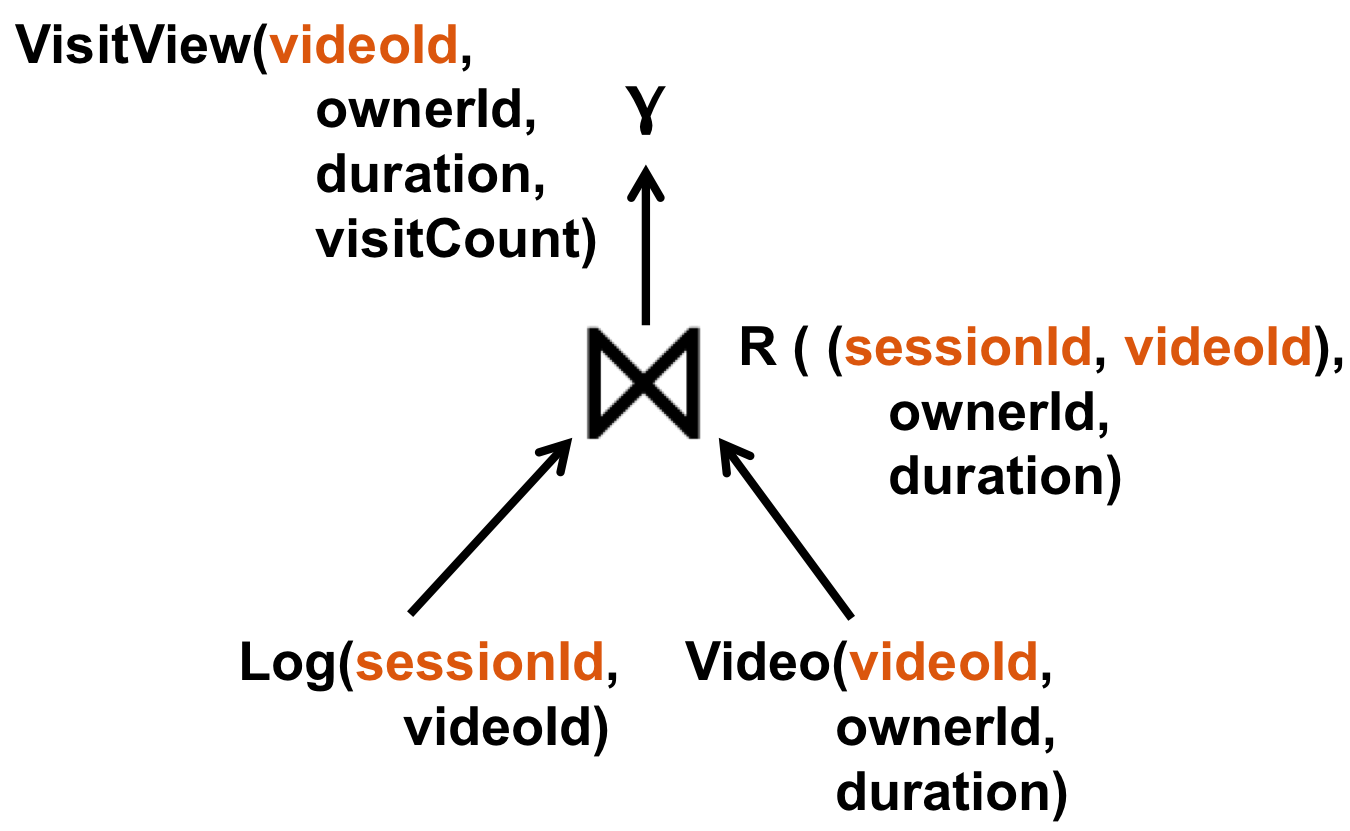
\includegraphics[scale=0.24]{figs/primary_key.png} \vspace{-.5em}
 \caption{Applying the rules described in Definition \ref{pk}, we illustrate how to assign a primary key to a view. \label{pk-fig}}\vspace{-1.5em}
\end{figure}

\begin{example}
A variant of our running example view that does not have a primary key is:
\begin{lstlisting}[mathescape,basicstyle={\scriptsize}]
CREATE VIEW visitView AS SELECT count(1) as visitCount
FROM Log, Video WHERE Log.videoId = Video.videoId
GROUP BY videoId
\end{lstlisting}
We illustrate this view in Figure \ref{pk-fig}.
To ensure that this view has a primary key for all subexpressions, we apply the rules pushing the primary keys from the base relations to the view.
Suppose there is a base relation, such as \tbl{Log}, that is missing a primary key (sessionId)\footnote{It does not make sense for Video to be missing a primary key in our running example due to the foreign key relationship}.
We can add this attribute by generating an increasing sequence of integers for each record in \tbl{Log}. 

Since both base tables \tbl{Video} and \tbl{Log} have primary keys videoId and sessionId respectively,
the result of the join will have a primary key (videoId, sessionId).
Then, since the group by attribute of the count is videoId, that is the primary key of the view.
Then, we can apply the rules above to propagate this key up the expression tree.
\end{example}

\subsection{Hashing Operator}
\label{push}
These primary keys define the provenance of a row $r$, which allows us to easily determine the set of rows in subexpressions that contribute
to $r$:
\begin{proposition}[Primary Key Provenance]\label{provalg}
Let $R$ and $U$ be relations as defined in Definition \ref{prov}. 
Let $A_R$ be the primary key set of $R$ and $A_U$ be the primary key 
set of $U$.
Define $r(A_R)$ as the primary key sets values for the row $r$.
$p_U(r)$ is defined as follows: (1) if $A_R \subseteq A_U$ then 
$\{u \in U: u(A_R) = r(A_R)\}$, (2) if $A_R \not \subseteq A_U$ then
return $U$.
\end{proposition}
We now explore how we can design a sampling technique to guarantee that all of the rows in Proposition \ref{provalg} are sampled if $r$ is sampled.
If we have a deterministic way of mapping a primary key defined in the previous subsection to Boolean true or false, we can ensure that all contributing rows are also sampled. 
To achieve this we use a hashing procedure.
Let us denote the hashing operator $\eta_{a, m}(R)$. 
For all tuples in R, this operator applies a hash function whose range is $[0,1]$ to primary key $a$ (which may be a set) and selects those records with hash value less than or equal to $m$.
If the hash function is sufficiently uniform, then the condition $h(a) \le m$ is true for close to a fraction $m$ of the rows. 
%This definition is without loss of generality for uniform hash function, as if we have a hash function whose range is the set of integers (as implemented in MySQL or Apache Hive) we can take the absolute value and divide by the maximum integer mapping this range back $[0,1]$. 

We push down the hashing operator through the query tree.
The further that we can push $\eta$ down the expression tree, the more operators can benefit from the sampling.
However, it is important to note that for some of the expressions, notably joins, the push down rules are more complex. 
It turns out in general we cannot push down even a deterministic sample through those expressions.
We formalize the push down rules below:
\begin{definition}[Hash Pushdown]
Let $a$ be a primary key of a materialized view. The following rules can be applied to push $\eta_{a, m}(R)$ down the expression tree of the maintenance strategy. 
\begin{itemize}[noitemsep]
\item $\sigma_{\phi}(R)$: Push $\eta$ through the expression.  
\item $\Pi_{(a_1,...,a_k)}(R)$: Push $\eta $ through if $a$ is in the projection.
\item $\bowtie_{\phi (r1,r2)}(R_1,R_2)$: Blocks $\eta $ in general. There are special cases below where push down is possible.
\item $\gamma_{f,A}(R)$: Push $\eta $ through if $a$ is in the group by clause $A$.
\item $R_1 \cup R_2$: Push $\eta $ through to both $R_1$ and $R_2$
\item $R_1 \cap R_2$: Push $\eta $ through to both $R_1$ and $R_2$
\item $R_1 - R_2$: Push $\eta $ through to both $R_1$ and $R_2$
\end{itemize}
\end{definition}
In special cases, we can push the hashing operator down through joins. 
Given the hash function $\eta_{a, m}(R)$:
\vspace{.25em}

{\noindent \textbf{Equality Join:}} If the join is an equality join and $a$ is one of the attributes in the equality join condition $R_1.a = R_2.b$, then $\eta$ can be pushed down to both $R_1$ and $R_2$. On $R_1$ the pushed down operator is $\eta_{a, m}(R_1)$ and on $R_2$ the operator is $\eta_{b, m}(R_2)$. This case often happens near the top of maintenance strategy expression tree where there is a equality outer join on the primary key of the stale view and a ``delta view''.

\vspace{.25em}

{\noindent \textbf{Foreign Key Join:}} If we have a join with two foreign-key relations $R_1$ (fact table with foreign key $a$) and $R_2$ (dimension table with primary key $b \subseteq a$) and we are sampling the key $a$, then we can push the sampling down to $R_1$. This is because we are guaranteed that for every $r_1\in R_1$ there is only one $r_2 \in R_2$. This case happens in our running example. If we sample the view on the primary key (\texttt{videoId}, \texttt{ownerId}, \texttt{language}, \texttt{duration}), since each video has only one owner, language and duration, we can push down the sampling of \texttt{videoId} to the \tbl{Log} relation and the \tbl{LogIns} table.

%A special case of the equality join rule is if we have a join with two foreign-key relations $R_1$ (fact table) and $R_2$ (dimension table). If we are sampling the foreign key (the primary key of the dimension table), then we can push down $\eta$ to both relations as in the equality join case. 

%\vspace{.25em}

%{\noindent \textbf{(Semi/Anti)-Join:}} Similarly, if we are hashing the primary key of a semi-join, we can always push $\eta$ down $R_1$. For anti-joins we can push $\eta$ down because we can rewrite the node as $R_1 - (R_1 \ltimes R_2) $ and apply the pushdown rules for set difference and Semi-Joins.

\vspace{0.25em}

The result of this hash operator pushdown on $\mathcal{M}$ is the cleaning expression $\mathcal{C}$. 
When applied to a stale sample of a view $\widehat{S}$, the database $\mathcal{D}$, and the delta relations $\partial \mathcal{D}$, it produces an up-to-date sample with sampling ratio $m$:
\[
\widehat{S}' = \mathcal{C}(\widehat{S},\mathcal{D},\partial \mathcal{D})
\]
Thus, it addresses Problem 1 from the previous section.

\begin{figure}[t] \vspace{-2em}
\centering
 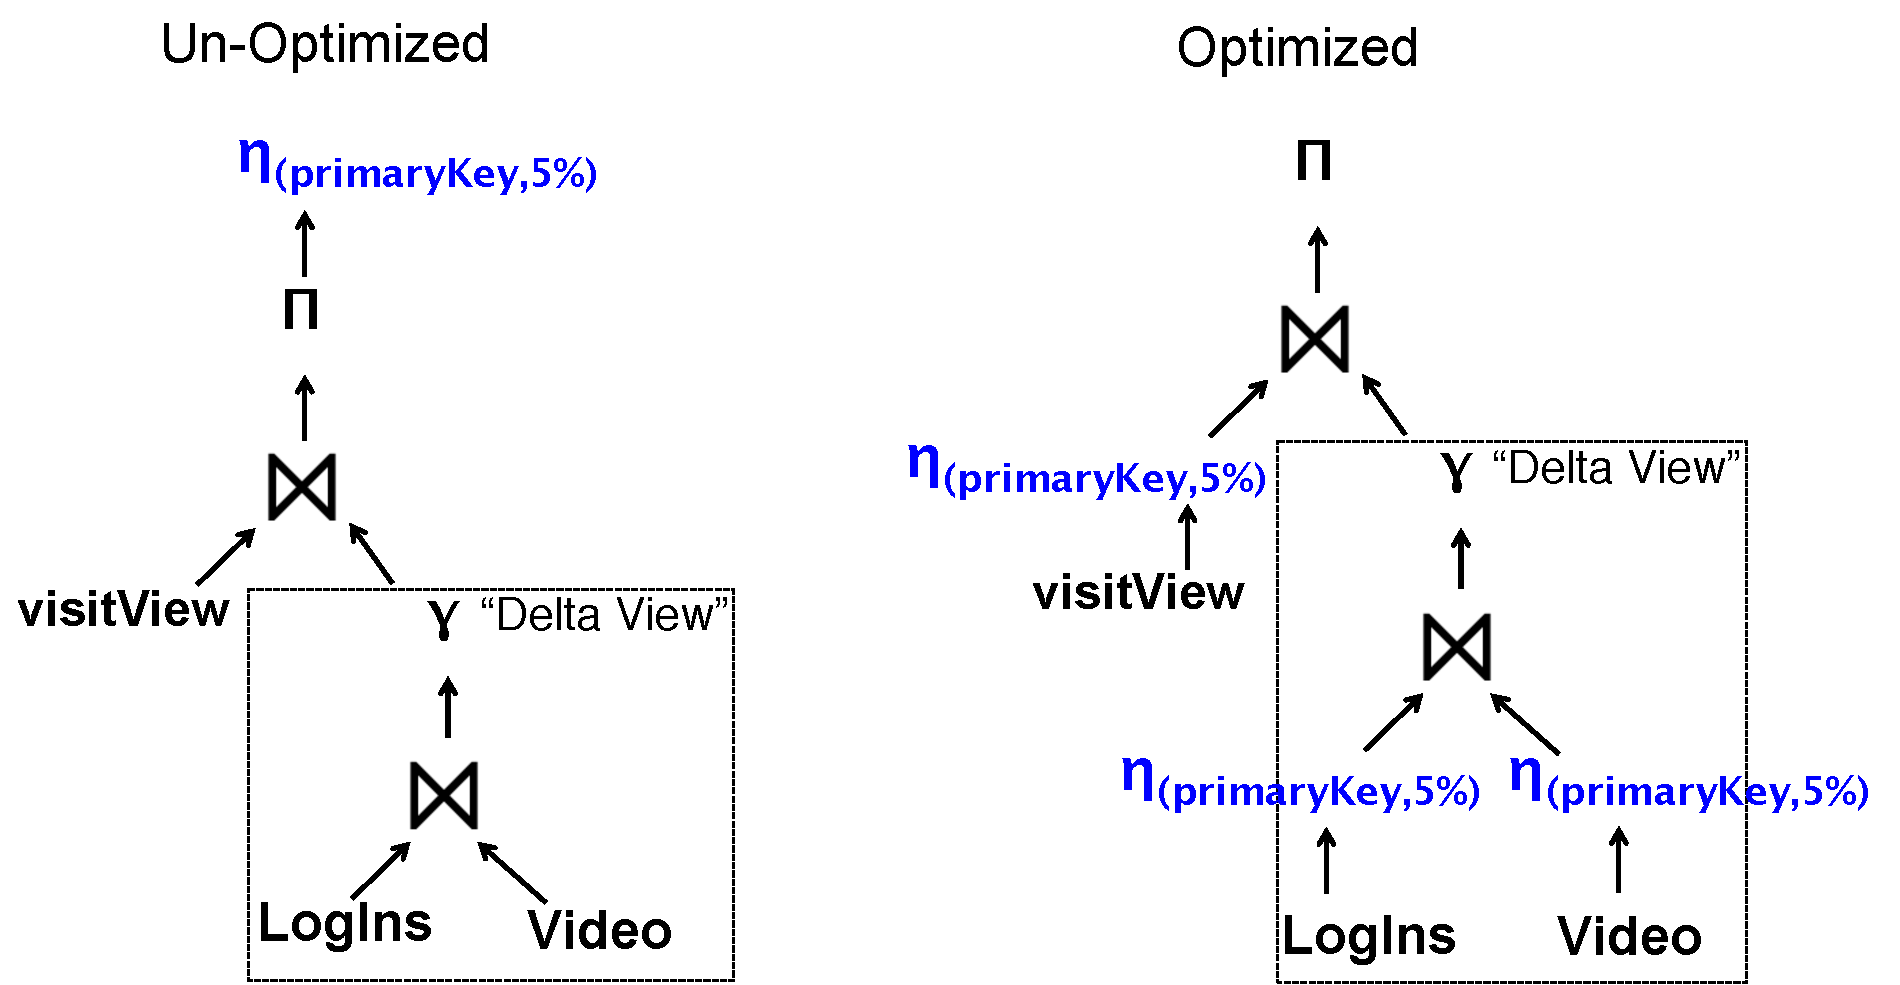
\includegraphics[scale=0.24]{figs/example_expression_tree_2.pdf} \vspace{-.5em}
 \caption{Applying the rules described in Section \ref{push}, we illustrate how to optimize the sampling of our example maintenance strategy. \label{exexpr2}}\vspace{-1em}
\end{figure}

\begin{example}
We illustrate our proposed approach on our example view \texttt{visitView} (Figure \ref{exexpr2}). 
The primary key for the view is the tuple (\texttt{videoId}) making that the primary key of the MV.
We start by applying the hashing operator to this key.
The next operator we see in the expression tree is a projection that increments the \texttt{visitCount} in the view, and this allows
for push down since primary key is in the projection.
The second expression is a hash of the equality join key which merges the aggregate from the ``delta view'' to the old view allowing us to push down on both branches of the tree using our special case for equality joins.
On the left side, we reach the stale view so we stop.
On the right side, we reach the aggregate query (count) and since the primary key is in group by clause, we can push down the sampling.
Then, we reach another point where we hash the equality join key allowing us to push down the sampling to the relations \tbl{LogIns} and \tbl{Video}.
\end{example}

\subsection{Corresponding Samples}
We started with a uniform random sample $\widehat{S}$ of the stale view $S$.
The hash push down allows us to efficiently materialize the sample $\widehat{S}'$.
$\widehat{S}'$ is a uniform random sample of the up-to-date view S.
While both of these samples are uniform random samples of their respective relations, 
the two samples are correlated since $\widehat{S}'$ is generated by cleaning $\widehat{S}$.
In particular, our hashing technique ensures that the primary keys in $\widehat{S}'$ depend on the primary keys in $\widehat{S}$.
Statistically, this positively correlates the query result $q(\widehat{S}')$ and $q(\widehat{S})$. 
We will see how this property can be leveraged to improve query estimation accuracy (Section \ref{re}). 

\begin{property}[Correspondence]
Suppose $\widehat{S'}$ and $\widehat{S}$ are uniform samples of $S'$ and $S$, respectively.  Let $u$ denote the primary key. We say $\widehat{S'}$ and $\widehat{S}$ correspond if and only if:
\vspace{-.25em}
\begin{itemize}[noitemsep]
\item Uniformity: $\widehat{S'}$ and $\widehat{S}$ are uniform random samples of $S'$ and $S$ respectively with a sampling ratio of $m$
\item Removal of Superfluous Rows: $D = \{\forall u \in \widehat{S} \wedge u \not\in S'\}$, $D \cap \widehat{S'} = \emptyset$ 
\item Sampling of Missing Rows: $I = \{\forall u \not\in S : u \in S'\}$, $\mathbb{E}(\mid I \cap \widehat{S'} \mid) = m\mid I \mid $ 
\item Key Preservation for Updated Rows: For all $u\in \widehat{S}$ and not in $D$ or $I$, $u\in \widehat{S}'$.
\end{itemize}
\vspace{-.25em}
\label{correspondence}
\end{property}







%\section{Delta-Algebra Optimizations}
As hinted in the previous section, optimizing joins is of particular interest. 
One of the most important use cases of materialized views to pre-compute expensive joins.
In \cite{DBLP:journals/vldb/KochAKNNLS14}, Koch et al. list the following properties of delta relations and joins:
\[ \Delta(R_1 \bowtie R_2) =  (R_1 \bowtie \Delta R_2) \dot{\cup} (\Delta R_1 \bowtie  R_2) \dot{\cup} (\Delta R_1 \bowtie  \Delta R_2)\]
\[ \nabla(R_1 \bowtie R_2) =  (R_1 \bowtie \nabla R_2) \dot{\cup} (\nabla R_1 \bowtie  R_2) \dot{\cup} (\nabla R_1 \bowtie  \nabla R_2)\]
When working with these delta relations, it would seem as though one join turns into three joins.
In this section, we explore when prune such expressions based on prior knowledge about the base relations and the updates.
\reminder{optimizations work only for insertions}

\subsection{Foreign-Key Constraints}

\reminder{the way that we model this subexpressions may violate constraints}

\textbf{Many-to-one insertion: } Suppose $R_1$ and $R_2$ have a foreign key constraint between them, and $R_1$ is the ``many" relation. Then, since every tuple in $R_1$ has to map to exactly one tuple in $R_2$, we know that insertions to $R_2$ could not affect existing tuples in $R_1$. Thus, we can prune the delta expression to:
\[ \Delta(R_1 \bowtie R_2) =  (\Delta R_1 \bowtie  R_2) \dot{\cup} (\Delta R_1 \bowtie  \Delta R_2)\]

\textbf{One-to-one insertion: } Suppose $R_1$ and $R_2$ have a foreign key constraint between them, and the relationship is exactly one-to-one. Then, since every tuple in $R_1$ has to map to exactly one tuple in $R_2$ and vice versa, we know that insertions to $R_2$ could not affect existing tuples in $R_1$ (and vice versa). Thus, we can prune the delta expression to:
\[ \Delta(R_1 \bowtie R_2) =  (\Delta R_1 \bowtie  \Delta R_2)\]

\subsection{Unique-Key Constraints and Stale Views}
In some cases, due to unique key constrains our delta expressions may be guaranteed to not overlap with another table. Consider the case of a simple selection view that selects records from a base relation. To update the view, we should take the union and not the join of the delta relation and the stale view. 
\[ \Delta(S) = S \dot{\cup} \Delta(S_{def}) \]
Recall our hash operator pushdown rules, we can push the operator to both S and the delta relation.
Thus, we can sample the stale view and the updates to the view independently.
Since S is already materialized, there is no need to sample S as that will not save any effort.
The implications of this optimization will be more evident in the following section about formulating a correction plan as this gives us the strong guarantee that our query time is strictly less than what it would be without sampling.

\subsection{Time/Causality Constraints}
In many important use cases such as log analysis, one or more of the base relations have time (e.g. timestamps or sequence numbers) as their primary key.
\textbf{$\theta$ join on time: } If we are applying a $\theta$ join, where the join key is time, then we can apply a similar optimization to the many-to-one insertion case.
\[ \Delta(R_1 \bowtie R_2) =   (\Delta R_1 \bowtie_{\theta}  R_2) \dot{\cup} (\Delta R_1 \bowtie_{\theta}  \Delta R_2)\]

\textbf{Aggregation on time: } Similarly, with group by aggregations if the group by expression is a monotonic function of time (e.g. count visits group by day), then we can apply a similar trick as used when there are unique key constraints and bound the effect of updating a stale view to the last group by key.




\section{Efficiency With Sampling}\label{dist-samp}
The model update received a sample with probabilities $p(\cdot)$.
For any distribution where  $p(\cdot) > 0$, we can preserve correctness.
\sys uses a sampling algorithm that selects the most valuable records to clean with higher probability. 

\subsection{Oracle Sampling Problem}
Recall that the convergence rate of an SGD algorithm is bounded by $\sigma^2$ which is the variance of the gradient.
Intuitively, the variance measures how accurately the gradient is estimated from a uniform sample.
Other sampling distributions, while preserving the sample expected value, may have a lower variance.
Thus, the oracle sampling problem is defined as a search over sampling distributions to find the minimum variance sampling distribution.

\begin{definition}[Oracle Sampling Problem]
Given a set of candidate dirty data $R_{dirty}$, $\forall r \in R_{dirty}$ find sampling probabilities $p(r)$ such that over all samples $S$ of size $k$ it minimizes:
\[
\mathbb{E}(\|g_S - g^*\|^2)
\]
\end{definition}
It can be shown that the optimal distribution over records in $R_{dirty}$ is probabilities proportional to:
\[
p_i \propto \|\nabla\phi(x^{(c)}_i,y^{(c)}_i,\theta^{(t)})\|
\]
We provide proofs and theoretical justification in appendix, but intuitively, records with higher gradients should be sampled with higher probability as they affect the update more significantly.
However, this cannot exclude records with lower gradients as that would induce a bias hurting convergence.
The problem is that this optimal distribution leads to a chicken-and-egg problem:
the optimal sampling distribution requires knowing $(x^{(c)}_i,y^{(c)}_i)$, however, cleaning is required to know those values.

\subsection{Dirty Gradient Solution}
Such an oracle does not exist, and one solution is to use the gradient w.r.t to the dirty data:
\[
p_i \propto \|\nabla\phi(x^{(d)}_i,y^{(d)}_i,\theta^{(t)})\|
\]
It turns out that this solution works reasonably well in practice on our experimental datasets and has been studied in Machine Learning as the Expected Gradient Length heuristic \cite{settles2010active}.
The contribution in this work is integrating this heuristic with statistically valid updates.
However, inutively, approximating the oracle as closely as possible can result in improved priortization.
The subsequent section describes two components, the detector and estimator, that can be used to achieve this.
Our experiments suggest up-to a 2x improvement in convergence when using these optional optimizations (Section \ref{comp}).
%\section{Further Optimizations}
As hinted in Section ??? optimizing joins is of particular interest. 
One of the most important use cases of materialized views to pre-compute expensive joins.
In \cite{DBLP:journals/vldb/KochAKNNLS14}, Koch et al. list the following properties of delta relations and joins:
\[ \Delta(R_1 \bowtie R_2) =  (R_1 \bowtie \Delta R_2) \dot{\cup} (\Delta R_1 \bowtie  R_2) \dot{\cup} (\Delta R_1 \bowtie  \Delta R_2)\]
\[ \nabla(R_1 \bowtie R_2) =  (R_1 \bowtie \nabla R_2) \dot{\cup} (\nabla R_1 \bowtie  R_2) \dot{\cup} (\nabla R_1 \bowtie  \nabla R_2)\]
When working with these delta relations, it would seem as though one join turns into three joins.
In this section, we explore when prune such expressions based on prior knowledge about the base relations and the updates.
In particular, we look at constraints on the primary key defined earlier in an insertion-only context.

\subsection{Foreign-Key Constraints}

\reminder{the way that we model this subexpressions may violate constraints}

\textbf{Many-to-one insertion: } Suppose $R_1$ and $R_2$ have a foreign key constraint between them, and $R_1$ is the ``many" relation. Then, since every tuple in $R_1$ has to map to exactly one tuple in $R_2$, we know that insertions to $R_2$ could not affect existing tuples in $R_1$. Thus, we can prune the delta expression to:
\[ \Delta(R_1 \bowtie R_2) =  (\Delta R_1 \bowtie  R_2) \dot{\cup} (\Delta R_1 \bowtie  \Delta R_2)\]

\textbf{One-to-one insertion: } Suppose $R_1$ and $R_2$ have a foreign key constraint between them, and the relationship is exactly one-to-one. Then, since every tuple in $R_1$ has to map to exactly one tuple in $R_2$ and vice versa, we know that insertions to $R_2$ could not affect existing tuples in $R_1$ (and vice versa). Thus, we can prune the delta expression to:
\[ \Delta(R_1 \bowtie R_2) =  (\Delta R_1 \bowtie  \Delta R_2)\]

\subsection{Time/Causality Constraints}
In many important use cases such as log analysis, one or more of the base relations have time (e.g. timestamps or sequence numbers) as their primary key.
\textbf{$\theta$ join on time: } If we are applying a $\theta$ join, where the join key is time, then we can apply a similar optimization to the many-to-one insertion case.
\[ \Delta(R_1 \bowtie R_2) =   (\Delta R_1 \bowtie_{\theta}  R_2) \dot{\cup} (\Delta R_1 \bowtie_{\theta}  \Delta R_2)\]

\textbf{Aggregation on time: } Similarly, with group by aggregations if the group by expression is a monotonic function of time (e.g. count visits group by day), then we can apply a similar trick as used when there are unique key constraints and bound the effect of updating a stale view to the last group by key.

\subsection{Unique-Key Constraints and Stale Views}
In some cases, due to unique key constraints our delta expressions may be guaranteed to not overlap with another table. 
This is of particular interest when such constraints appear at the highest level of our maintenance plan.
Consider the case of a simple selection view that selects records from a base relation. 
To update the view, we should take the union and not the join of the delta relation and the stale view. 
\[ \Delta(S) = S \dot{\cup} \Delta(S_{def}) \]
Recall our hash operator pushdown rules, we can push the operator to both S and the delta relation.

Thus, we can sample the stale view and the updates to the view independently.
The implications of this optimization will be more evident in the following section about formulating a correction plan as this gives us the strong guarantee that our query time is strictly less than what it would be without sampling:
\[O(\mid S \mid + m \cdot \mid \Delta S' \mid) \le O(\mid S \mid + \cdot \mid \Delta ' \mid)\]





\vspace{-.5em}
\section{Outlier Indexing}\label{outlier}
Sampling is known to be sensitive to outliers \cite{clauset2009power, chaudhuri2001overcoming}.
Power-laws and other long-tailed distributions are common in practice \cite{clauset2009power}.
We address this problem using a technique called outlier indexing which has been applied in AQP \cite{chaudhuri2001overcoming}.
The basic idea is that we create an index of outlier records (records whose attributes deviate from the mean value greatly) and ensure that these records are included in the sample, since these records greatly increase the variance of the data. 
%Furthermore, since they are likely rare the probability of sampling them is low leading to wildly varying estimates.  
However, as this has not been explored in the materialized view setting there are new challenges in using this index for improved result accuracy.

\subsection{Indices on the Base Relations}
In \cite{chaudhuri2001overcoming}, the authors applied outlier indexing to improve the accuracy of AQP on base relations.
%We apply a similar technique, however, their problem setting is different in a few ways.
%First, in the AQP setting, queries are issued to base relations.
In our problem, we issue queries to materialized views.
We need to define how to propagate information from an outlier index on the base relation to a materialized view.

The first step is that the user selects an attribute of any base relation to index and specifies a threshold $t$ and a size limit $k$.
In a single pass of updates (without maintaining the view), the index is built storing references to the records with attributes greater than $t$.
If the size limit is reached, the incoming record is compared to the smallest indexed record and if it is greater then we evict the smallest record.
The same approach can be extended to attributes that have tails in both directions by making the threshold $t$ a range, which takes the highest and the lowest values.
However, in this section, we present the technique as a threshold for clarity.

There are many approaches to select a threshold.
We can use prior information from the base table, a calculation which can be done in the background during the periodic maintenance cycles.
If our size limit is $k$, for a given attribute we can select the the top-k records with that attributes.
Then, we can use that top-k list to set a threshold for our index. 
Then, the attribute value of the lowest record becomes the threshold $t$.
Alternatively, we can calculate the variance of the attribute and set the threshold to represent $c$ standard deviations above the mean.

This threshold can be adaptively set at each maintenance period to include more or less outliers.
The caveat is that the outlier index should not be too expensive to calculate nor should it be too large as it negates the performance benefits of sampling.  
The query processing approach that we propose in the following sub-sections is agnostic to how we choose this threshold.
In fact, our approach allows us to incorporate any deterministic subset into our sample-based correction calculations.

\subsection{Adding Outliers to the Sample}
%Given this index, the next question is how we can use this information in our materialized views.
%We ensure that any row in a materialized view that is derived from an indexed record is guaranteed to be in the sample.
%This problem is sort of an inverse to the efficient sampling problem studied in Section~\ref{sampling}.
We need to propagate the indices upwards through the expression tree.
%The next challenge is the outlier index must not require any additional effort to materialize.
We add the condition that the only eligible indices are ones on base relations that are being sampled (i.e., we can push the hash operator down to that relation).
Therefore, in the same iteration as sampling, we can also test the index threshold and add records to the outlier index. 
We formalize the propagation property recursively. 
Every relation can have an outlier index which is a set of attributes and a set of records that exceed the threshold value on those attributes.
The main idea is to treat the indexed records as a sub-relation that gets propagated upwards with the maintenance strategy.
\begin{definition}[outlier index pushup]
Define an outlier index to be a tuple of a set of indexed attributes, and a set of records $(I,O)$. The outlier index propagates upwards with the following rules: 
\begin{itemize}[noitemsep]
\item Base Relations: Outlier indices on base relations are pushed up only if that relation is being sampled, i.e., if the sampling operator can be pushed down to that relation.
\item $\sigma_{\phi}(R)$: Push up with a new outlier index and apply the selection to the outliers $(I,\sigma_{\phi}(O))$ 
\item $\Pi_{(a_1,...,a_k)}(R)$: Push upwards with new outlier index $(I \cap (a_1,...,a_k), O)$.
\item $\bowtie_{\phi (r1,r2)}(R_1,R_2)$: Push upwards with new outlier index $(I_{1} \cup I_{2}, O_1 \bowtie O_2)$. 
\item $\gamma_{f,A}(R)$: For group-by aggregates, we set $I$ to be the aggregation attribute. For the outlier index, we do the following steps. (1) Apply the aggregation to the outlier index $\gamma_{f,A}(O)$, (2) for all distinct $A$ in $O$ select the row in $\gamma_{f,A}(R)$ with the same $A$, and (3) this selection is the new set of outliers $O$. 
\item $R_1 \cup R_2$: Push up with a new outlier index $(I_1 \cap I_2, O_1 \cup O_2)$. The set of index attributes is combined with an intersection to avoid missed outliers.
\item $R_1 \cap R_2$: Push up with a new outlier index $(I_1 \cap I_2, O_1 \cap O_2)$.
\item $R_1 - R_2$: Push up with a new outlier index $(I_1 \cup I_2, O_1 - O_2)$.
\end{itemize}
\end{definition}

For all outlier indices that can propagate to the view (i.e., the top of the tree), we get a final set $O$ of records. 
Given these rules, $O$ is, in fact, a subset of our materialized view $S'$.
Thus, our query processing can take advantage of the theory described in the previous section to incorporate the set $O$ into our results.
We implement the outlier index as an additional attribute on our sample with a boolean flag true or false if it is an outlier indexed record.
If a row is contained both in the sample and the outlier index, the outlier index takes precedence.
This ensures that we do not double count the outliers.

\subsection{Query Processing}\label{oqp} 
For result estimation, we can think of our sample $\hat{S'}$ and our outlier index $O$ as two distinct parts.
Since $O \subset S'$, and we give membership in our outlier index precedence, our sample is actually a sample restricted to the set $\widehat{(S'-O)}$. 
The outlier index has two uses: (1) we can query all the rows that correspond to outlier rows, 
and (2) we can improve the accuracy of our \emph{aggregation} queries.
To query the outlier rows, we can select all of the rows in the materialized view that are flagged as outliers, and these rows are guaranteed to be up-to-date.

For (2), we can also incorporate the outliers into our correction estimates.  
For a given query, let $c_{reg}$ be the correction calculated on $\widehat{(S'-O)}$ using the technique proposed in the previous section and adjusting the sampling ratio $m$ to account for outliers removed from the sample.
We can also apply the technique to the outlier set $O$ since this set is deterministic the sampling ratio for this set is $m=1$, and we call this result $c_{out}$.
Let $N$ be the count of records that satisfy the query's condition and $l$ be the number of outliers that satisfy the condition.
Then, we can merge these two corrections in the following way:
$
 v = \frac{N-l}{N}c_{reg} + \frac{l}{N}c_{out}
$.
For the queries in the previous section that are unbiased, this approach preserves unbiasedness.
Since we are averaging two unbiased estimates $c_{reg}$ and $c_{out}$, the linearity of the expectation operator preserves this property.
Furthermore, since $c_{out}$ is deterministic (and in fact its bias/variance is 0), $c_{reg}$ and $c_{out}$ are uncorrelated making the bounds described in the previous section applicable as well.

\begin{example}
Suppose, we want to use outlier indexing to process the query in the previous section on \tbl{visitView}.
We chose an attribute in the base data to index, for example \texttt{duration}, and an example threshold of 1.5 hours.
We first push the index through the join of \tbl{Log} and \tbl{Video}.
Then, we reach the group by aggregate, where we select all the distinct groups (videos) for which 
the duration is longer than 1.5 hours.
This materializes the entire set of rows whose duration is longer than 1.5 hours.
For SVC+AQP, we run the query on the set of clean rows with durations longer than 1.5 hours.
Then, we use the update rule in Section \ref{oqp} to update the result based on the number of records in the index and the total size of the view.
For SVC+CORR, we additionally run the query on the set of dirty rows with durations longer than 1.5 hours and take the difference between SVC+AQP.
As in SVC+AQP, we use the update rule in Section \ref{oqp} to update the result based on the number of records in the index and the total size of the view.
\end{example}

%sum of uncorrelated unbiased estimates since one is deterministic.

%See \cite{chaudhuri2001overcoming} for additional query processing details.
%\section{Extensions}\label{sec:ext}
\subsection{Hash-Operator}
We defined a concept of tuple-lineage with primary keys.
However, a curious property of the deterministic hashing technique is that we can actually hash any attribute while retain the important
statistical properties.
This is because a uniformly random sample of any attribute (possibly not unique) still includes every individual row with the same probability.  
A consequence of this is that we can push down the hashing operator through arbitrary equality joins (not just many-to-one) by hashing the join key.

We defer further exploration of this property to future work as it introduces new tradeoffs.
For example, sampling on a non-unique key, while unbiased in expectation, has higher variance in the size of the sample.
Happening to hash a large group may lead to decreased performance. 

Suppose our keys are duplicated $\mu_k$ times on average with variance $\sigma_k^2$, then the variance of the
sample size is for sampling fraction $m$:
\[m(1-m)\mu_k^2+(1-m)\sigma_k^2\]
This equation is derived from the formula for the variance of a mixture distribution.
In this setting, our sampling would have to consider this variance against the benefits of pushing the hash operator further down the query tree. 

\subsection{Sampling Updates vs. Sampling Views}
In SVC, we sample from views and work backwards through the view definition using relational algebra.
An alternative approach is to sample the base relations of the view.
However, this approach quickly leads to some bottlenecks.
For example, if our view is an aggregate view with a nested selection, we can easily construct a distinct count problem rendering any aggregate query inestimable \cite{DBLP:conf/pods/CharikarCMN00}.

For some types of views, this model is actually a special case of SVC.
For views where primary key of the base relations is an attribute of the view, we can sample those attributes.
We can quickly see that based on our pushdown rules if there is a nested aggregate query, pushdown can fail in general.
However, re-writing views and queries to better support sampling is an interesting avenue of future work.

\subsection{Multi-View Setting}
In a production environment, the database system might have many materialized views. 
With the sampling ratio, SVC gives the database administrator an additional degree of freedom to adjust throughput, storage, and accuracy.
The sampling ratio of each view can be adaptively adjusted to suit the workload.

We can pose minimizing the expected estimation error as a Geometric Convex Program.
In one time period, if view $i$ has an expected cardinality of $N_i$, an average query variance of $\alpha_i$, a sampling ratio of $m_i$, there is a total space budget of $B$, the cost for update is $C_i$ secs/Record and throughput demand of $D$ latency:
\[\arg \min_{m_i} \sum_i \frac{\alpha_i}{m_i \cdot N_i}\]
\[\text{subject to:} \sum_i m_i \cdot N_i \le B \]
\[\sum_i m_i\cdot N_i \cdot C_i \le D \]






\section{Experiments}\label{eval}
First, the experiments evaluate how various types of corrupted data benefit from data cleaning.
Next, the experiments explore different prioritization and model update schemes for progressive data cleaning.
Finally, \sys is evaluated end-to-end in a number of real-world data cleaning scenarios.

\subsection{Experimental Setup and Notation}
The main metric for evaluation is a relative measure of the trained model and the model if all of the data is cleaned.

\vspace{0.5em}

\noindent\textbf{Relative Model Error. } Let $\theta$ be the model trained on the dirty data, and let $\theta^*$ be the model trained on the same data if it was cleaned. Then the model error is defined as $\frac{\|\theta - \theta^*\|}{\|\theta^*\|}$.

\subsubsection{Scenarios}
%\vspace{0.5em}

%\noindent\textbf{Housing: } In this dataset, our task is to predict housing prices from 13 numerical and categorical covariates. There are 550 data points in this dataset. The model is a Logistic Regression classifier which predicts if the house price is greater than \$500k.

\vspace{0.25em}

\noindent\textbf{Income Classification (Adult): } In this dataset of 45,552 records, the task is to predict the income bracket (binary) from 12 numerical and categorical covariates with an SVM classifier. 

\vspace{0.25em}

\noindent\textbf{Seizure Classification (EEG): } In this dataset, the task is to predict the onset of a seizure (binary) from 15 numerical covariates with a thresholded Linear Regression. There are 14980 data points in this dataset. This classification task is inherently hard with an accuracy on completely clean data of only 65\%.

\vspace{0.25em}

\noindent\textbf{Handwriting Recognition (MNIST) \footnote{\scriptsize\url{http://ufldl.stanford.edu/wiki/index.php/Using_the_MNIST_Dataset}}: } In this dataset, the task is to classify 60,000 images of handwritten images into 10 categories with an one-to-all multiclass SVM classifier. The unique part of this dataset is the featurized data consists of a 784 dimensional vector which includes edge detectors and raw image patches. 

\vspace{0.25em}

\noindent\textbf{Dollars For Docs: } The dataset has 240,089 records with 5 textual attributes and one numerical attribute.
The dataset is featurized with bag-of-words featurization model for the textual attributes which resulted in a 2021 dimensional feature vector, and a binary SVM is used to classify the status of the medical donations.

\subsubsection{Compared Algorithms}
\noindent Here are the alternative methodologies evaluated in the experiments:

\vspace{0.25em}

\noindent\textbf{Robust Logistic Regression \cite{feng2014robust}. } Feng et al. proposed a variant of logistic regression that is robust to outliers. We chose this algorithm because it is a robust extension of the convex regularized loss model, leading to a better apples-to-apples comparison between the techniques. (See details in Appendix \ref{rlogit})  

\vspace{0.25em}

\noindent\textbf{Discarding Dirty Data. } As a baseline, dirty data is discarded.

\vspace{0.25em}

\noindent\textbf{SampleClean (SC) \cite{wang1999sample}. } SampleClean takes a sample of data, applies data cleaning, and then trains a model to completion on the sample.

\vspace{0.25em}

\noindent\textbf{Active Learning (AL) \cite{guillory2009active}. } An Active Learning algorithm that integrates with stochastic optimization (See details in Appendix \ref{al}). 

\vspace{0.25em}

\noindent\textbf{ActiveClean Oracle (AC+O): } In \sys Oracle, instead of an estimation step, the true clean value is used to evaluate the theoretical ideal performance of \sys.

\subsection{Does Data Cleaning Matter?}
The first experiment evaluates the benefits of data cleaning on two of the example datasets (EEG and Adult).
This is done without sampling to understand which types of data corruption are amenable to data cleaning and which are better suited for robust statistical techniques.
The experiment compares four schemes: (1) full data cleaning  , (2) baseline of no cleaning, (3) discarding the dirty data, and (4) robust logistic regression,. We corrupted 5\% of the training examples in each dataset in two different ways:

\vspace{0.5em}

\noindent\textbf{Random Corruption: } Simulated high-magnitude random outliers. 5\% of the examples are selected at random and a random feature is replaced with 3 times the highest feature value.

\vspace{0.5em}

\noindent\textbf{Systematic Corruption: } Simulated innocuous looking (but still incorrect) systematic corruption. The model is trained on the clean data, and the three most important features (highest weighted) are identified. The examples are sorted by each of these features and the top examples are corrupted with the mean value for that feature (5\% corruption in all). 
It is important to note that examples can have multiple corrupted features.

\begin{figure}[t]
\centering
 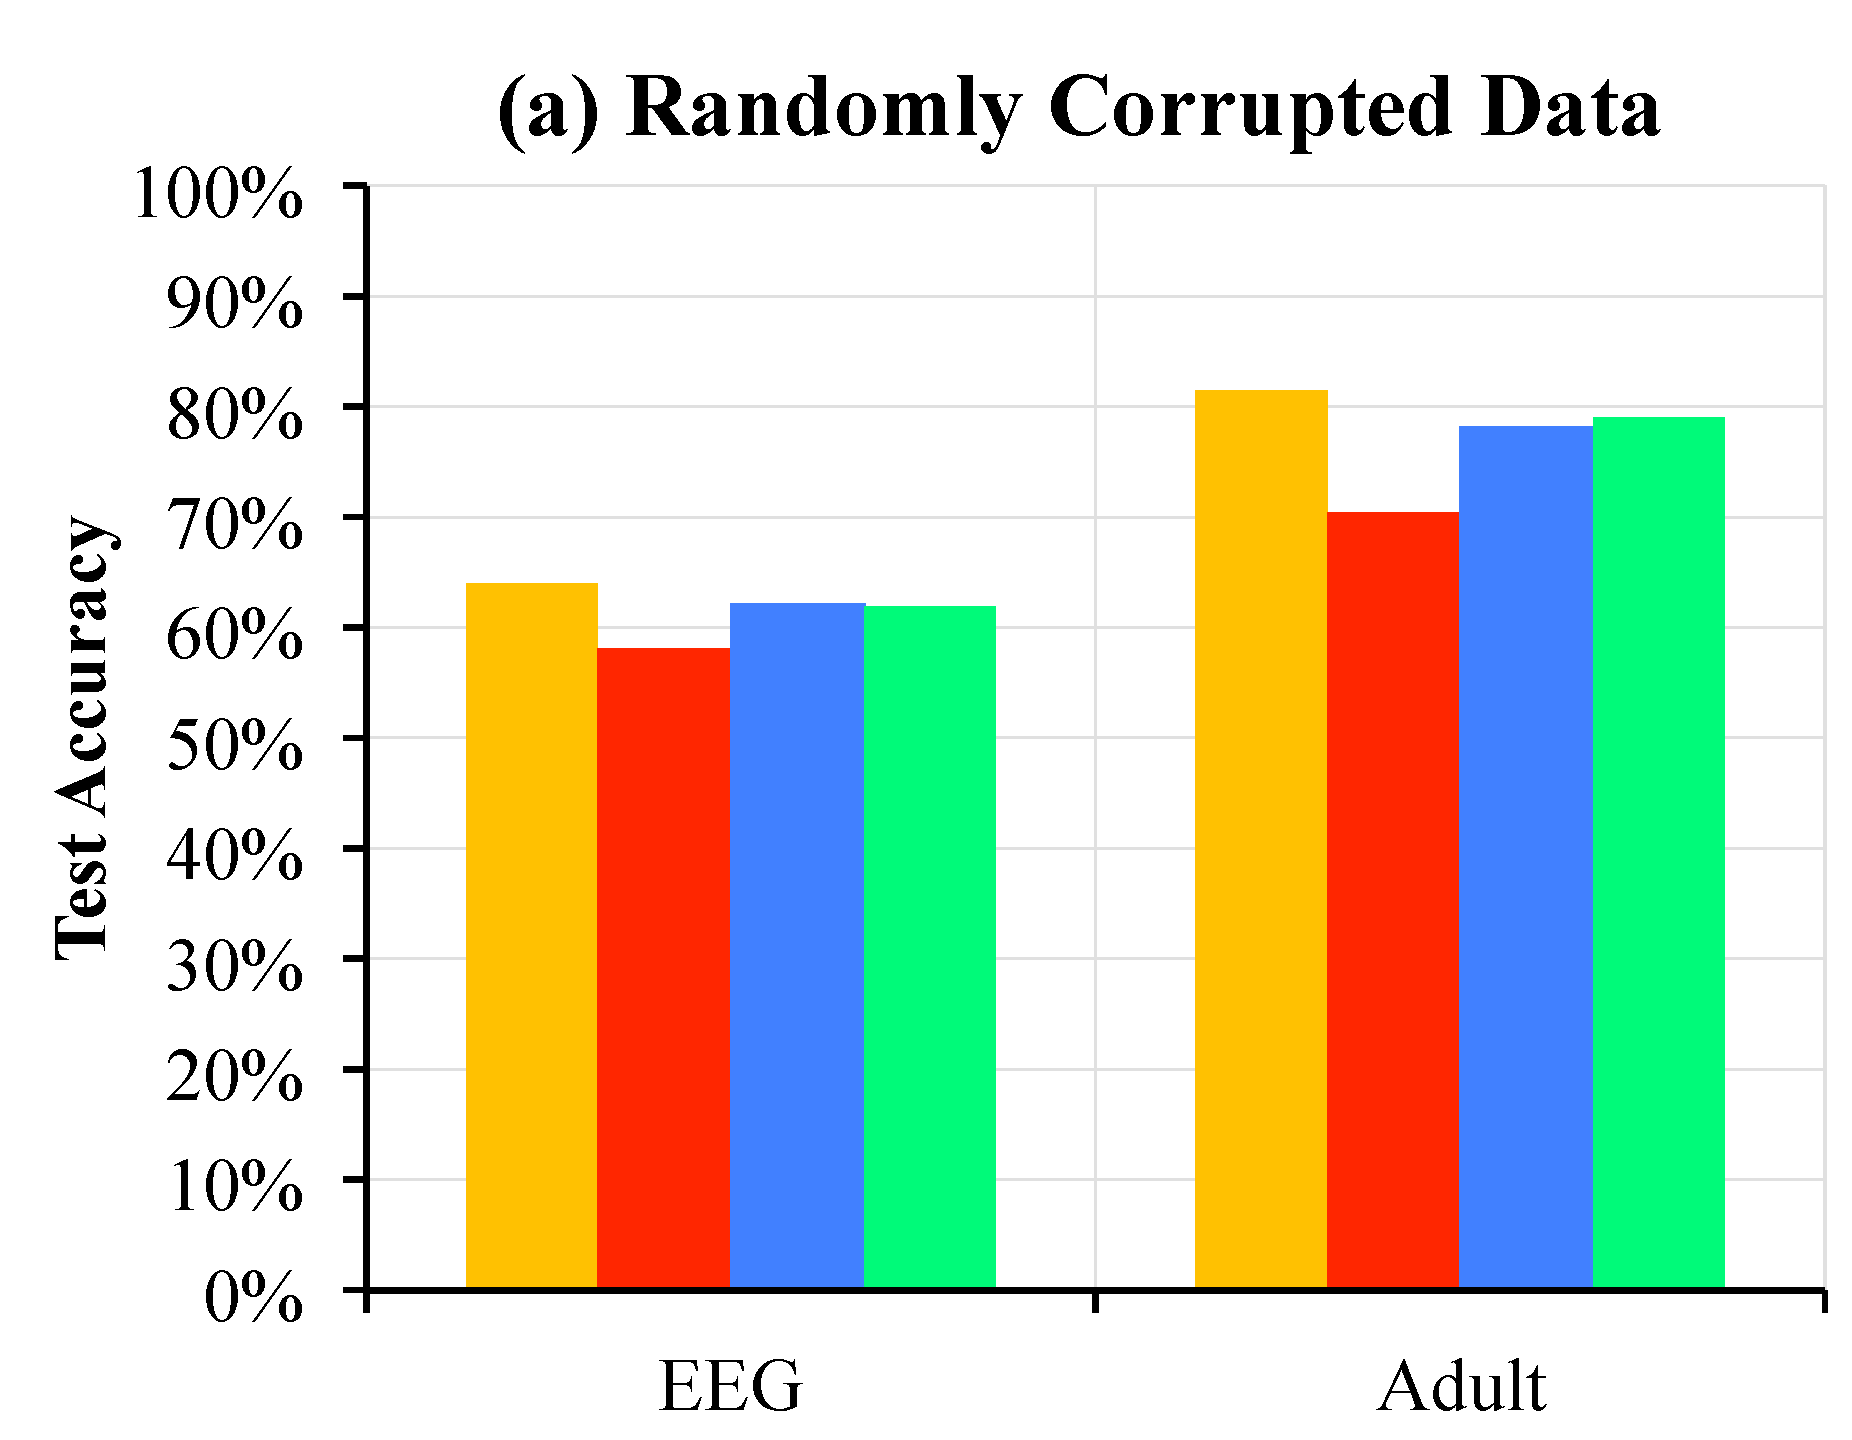
\includegraphics[width=0.49\columnwidth]{exp/exp2.pdf}
 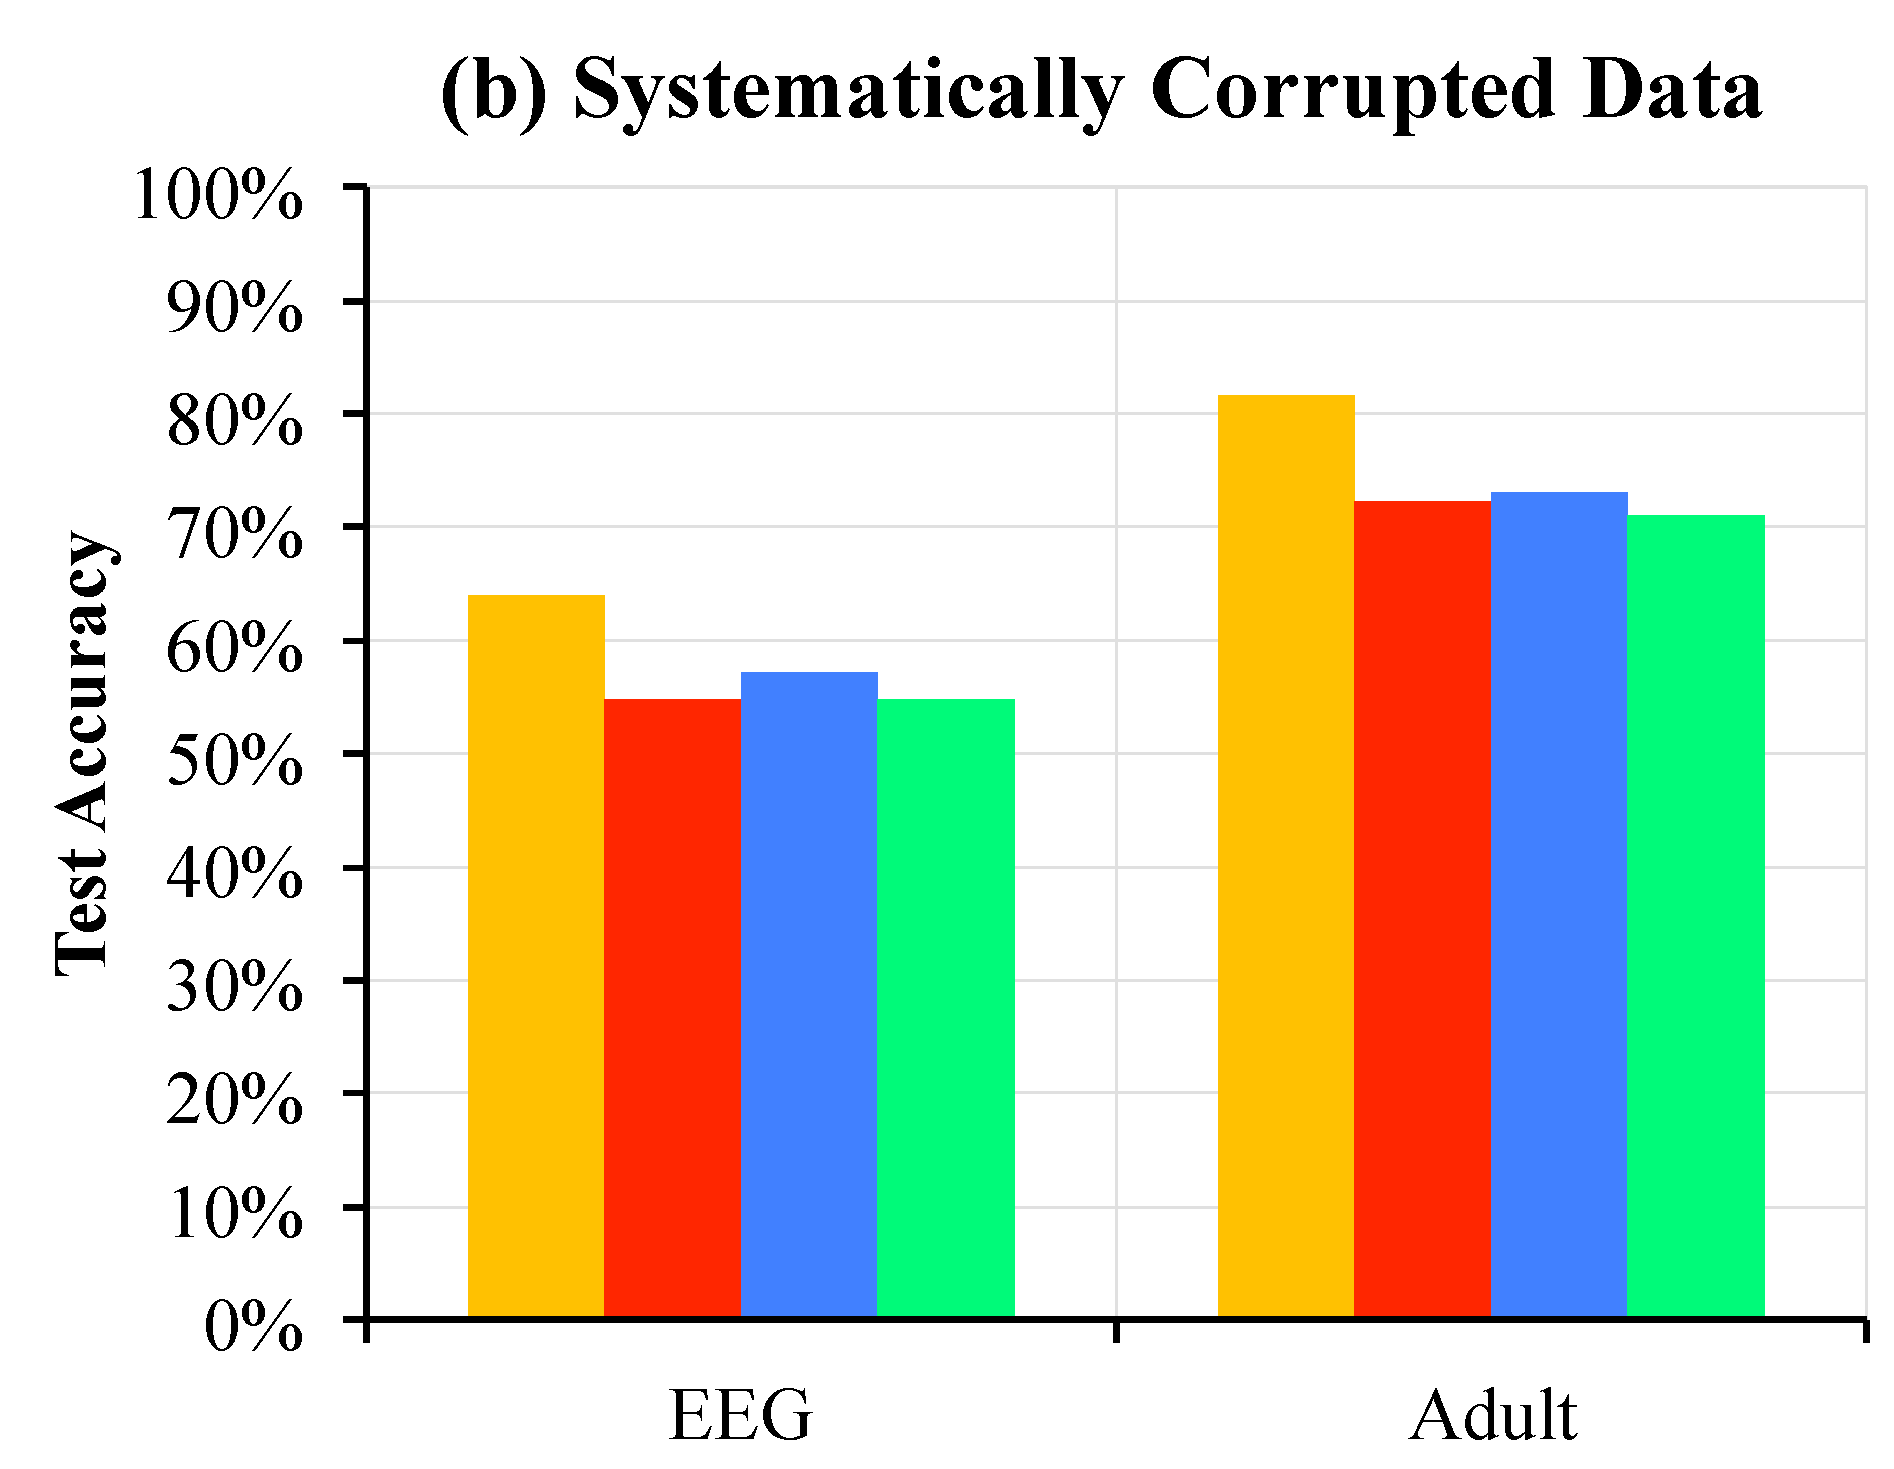
\includegraphics[width=0.49\columnwidth]{exp/exp1.pdf}
 
\includegraphics[width=0.5\columnwidth]{exp/legend-1.png}\vspace{-1em}
 \caption{(a) Robust techniques and discarding data work when corrupted data are random and look atypical. (b) Data cleaning can provide reliable performance in both the systematically corrupted setting and randomly corrupted setting.\label{sys-rand}}\vspace{-1.5em}
\end{figure}

Figure \ref{sys-rand} shows the test accuracy for models trained on both types of data with the different techniques.
The robust method performs well on the random high-magnitude outliers with only a 2.0\% reduction in clean test accuracy for EEG and 2.5\% reduction for Adult.
In the random setting, discarding dirty data also performs relatively well.
However, the robust method falters on the systematic corruption with a 9.1\% reduction in clean test accuracy for EEG and 10.5\% reduction for Adult.
%Data cleaning is the most reliable option across datasets and corruption types.
The problem is that without cleaning, there is no way to know if the corruption is random or systematic and when to trust a robust method.
While data cleaning requires more effort, it provides benefits in both settings.
In the remaining experiments, unless otherwise noted, the experiments use systematic corruption.

\noindent \emph{Summary: A 5\% systematic corruption can introduce a 10\% reduction in test accuracy even when using a robust method.}

\subsection{\sys: \protect\textit{\large A Priori} Detection}
The next set of experiments evaluate different approaches to cleaning a sample of data compared to \sys using \emph{a priori} detection.
\emph{A priori} detection assumes that all of the corrupted records are known in advance but their clean values are unknown. 

\subsubsection{Active Learning and SampleClean}
The next experiment evaluates the samples-to-error tradeoff between four alternative algorithms: \sys (AC), SampleClean, Active Learning, and \sys+Oracle (AC+O).
Figure \ref{prio-perf} shows the model error and test accuracy as a function of the number of cleaned records.
In terms of model error, \sys gives its largest benefits for small sample sizes.
For 500 cleaned records of the Adult dataset, \sys has 6.1x less error than SampleClean and 2.1x less error than Active Learning.
For 500 cleaned records of the EEG dataset, \sys has 9.6x less error than SampleClean and 2.4x less error than Active Learning.
Both Active Learning and \sys benefit from the initialization with the dirty model as they do not retrain their models from scratch, and \sys improves on this performance with detection and error estimation.
Active Learning has no notion of dirty and clean data, and therefore prioritizes with respect to the dirty data.
These gains in model error also correlate well to improvements in test error (defined as the test accuracy difference w.r.t cleaning all data).
The test error converges more quickly than model error, emphasizing the benefits of progressive data cleaning, since it is not neccessary to clean all the data to get a model with essentially the same performance as the clean model.
For example, to achieve a test error of 1\% on the Adult dataset, \sys cleans 500 fewer records than Active Learning.


\vspace{0.25em}

\noindent \emph{Summary: \sys with a priori detection returns results that are more than 6x more accurate than SampleClean and 2x more accurate than Active Learning for cleaning 500 records.}

\begin{figure}[t]
\centering\vspace{-1em}
 %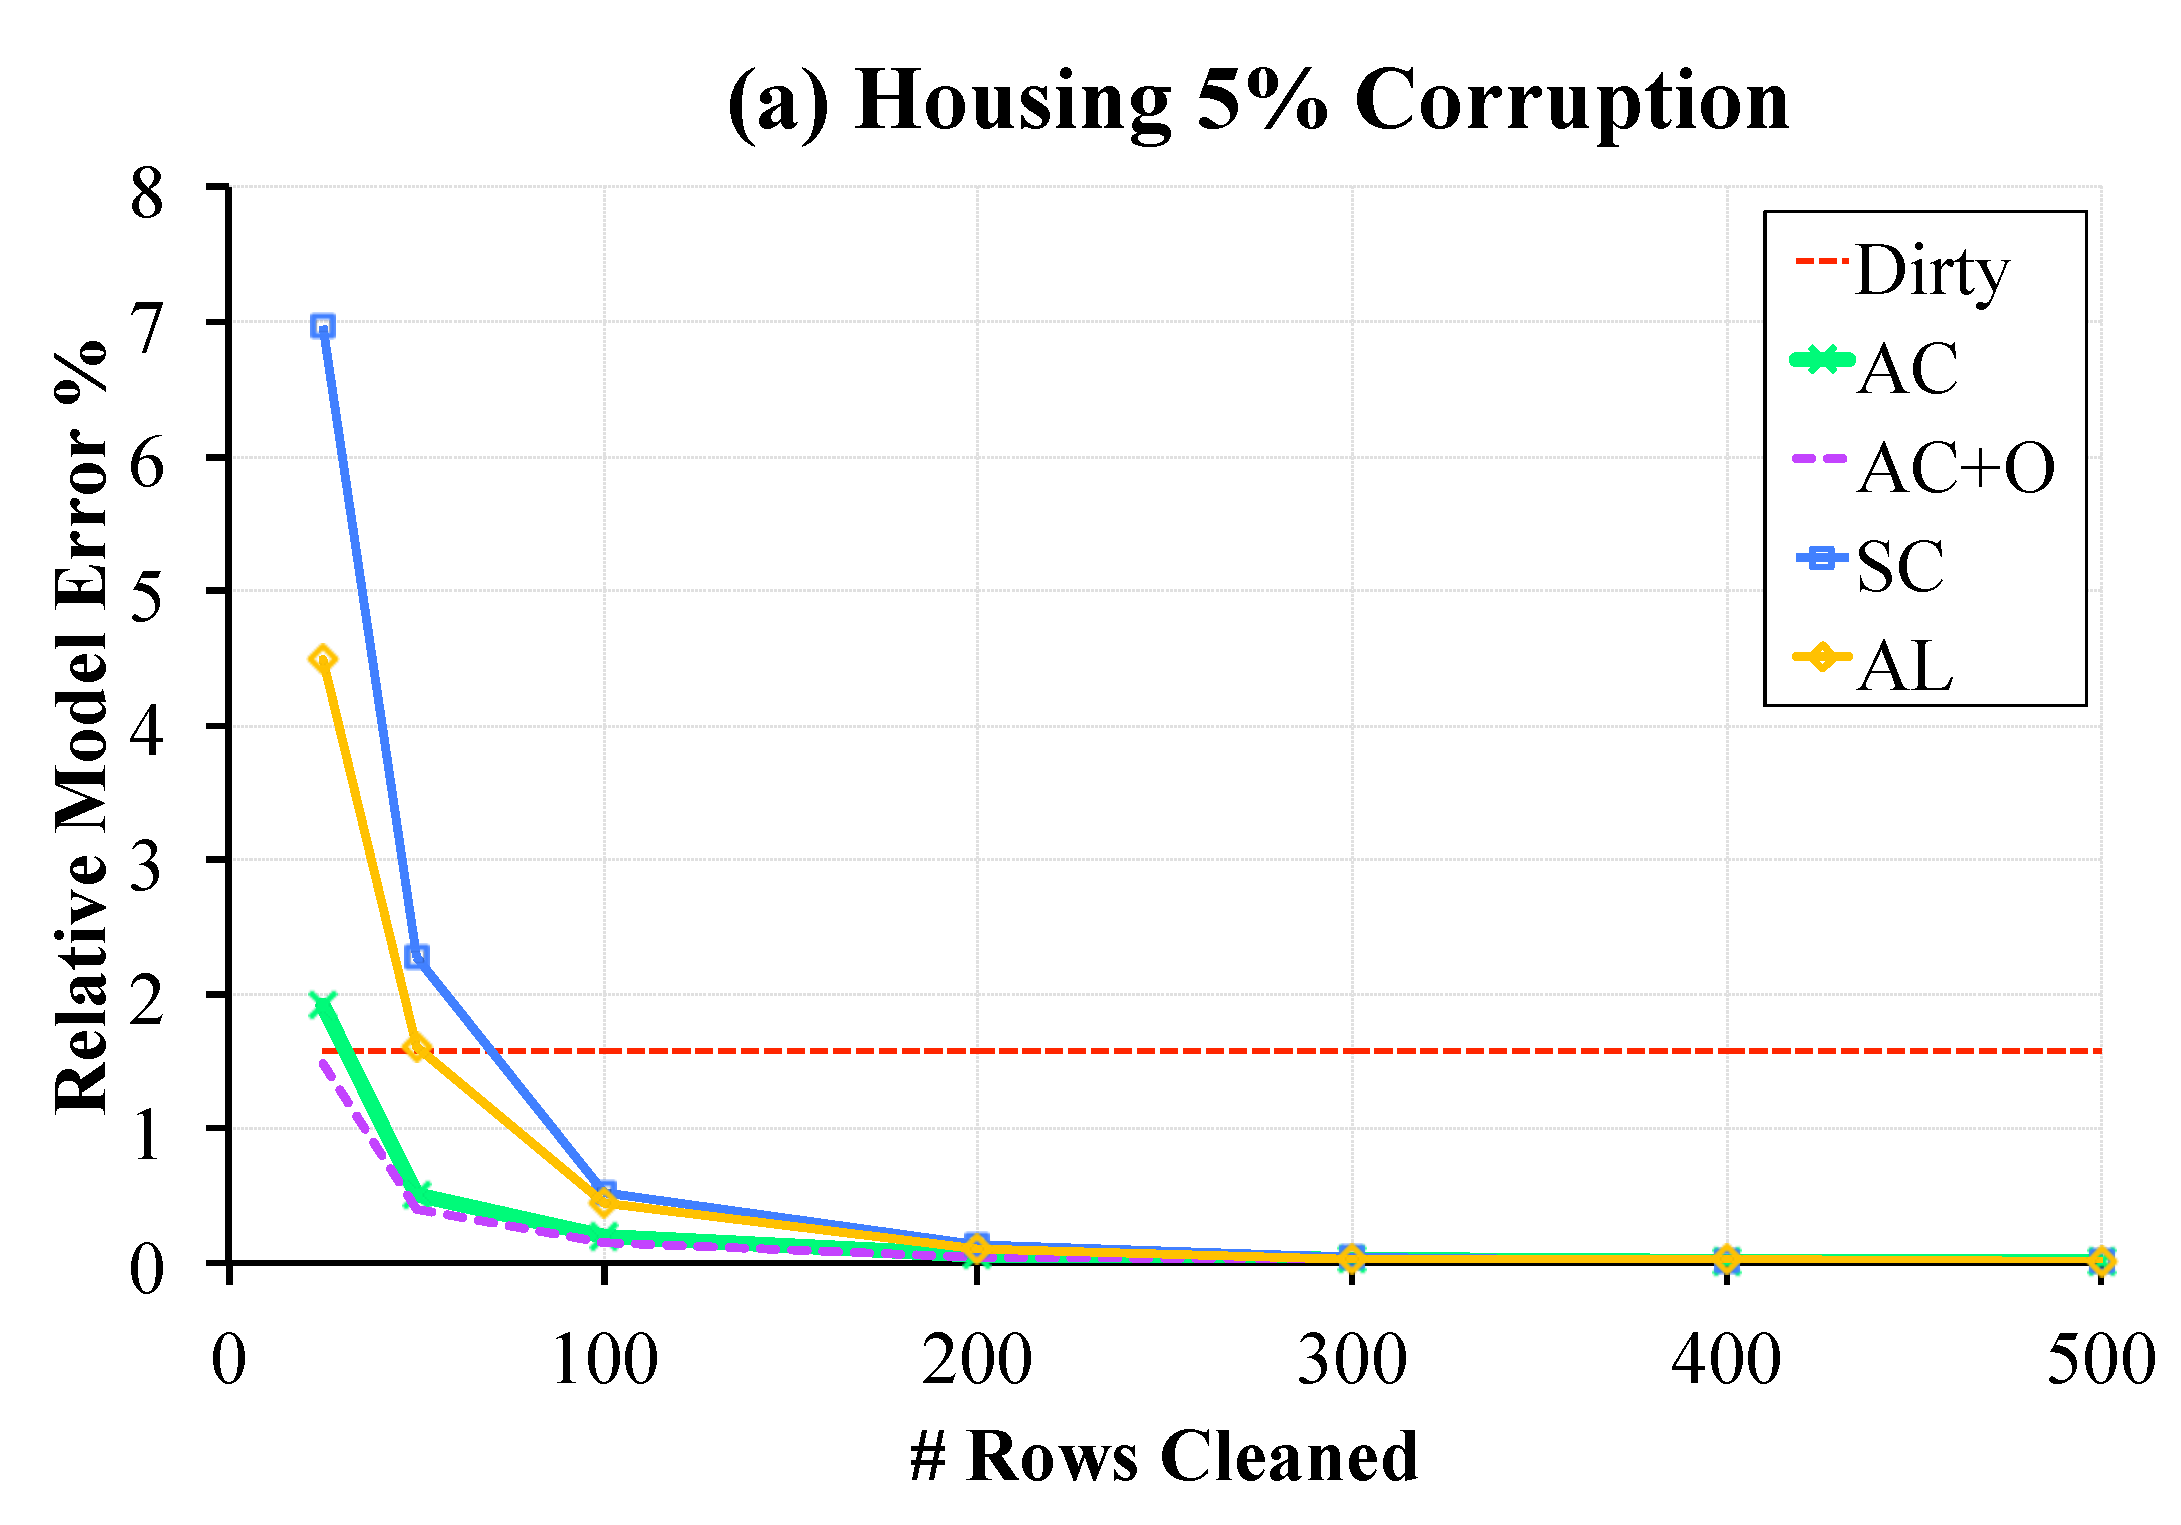
\includegraphics[scale=0.15]{exp/exp3a.pdf}
 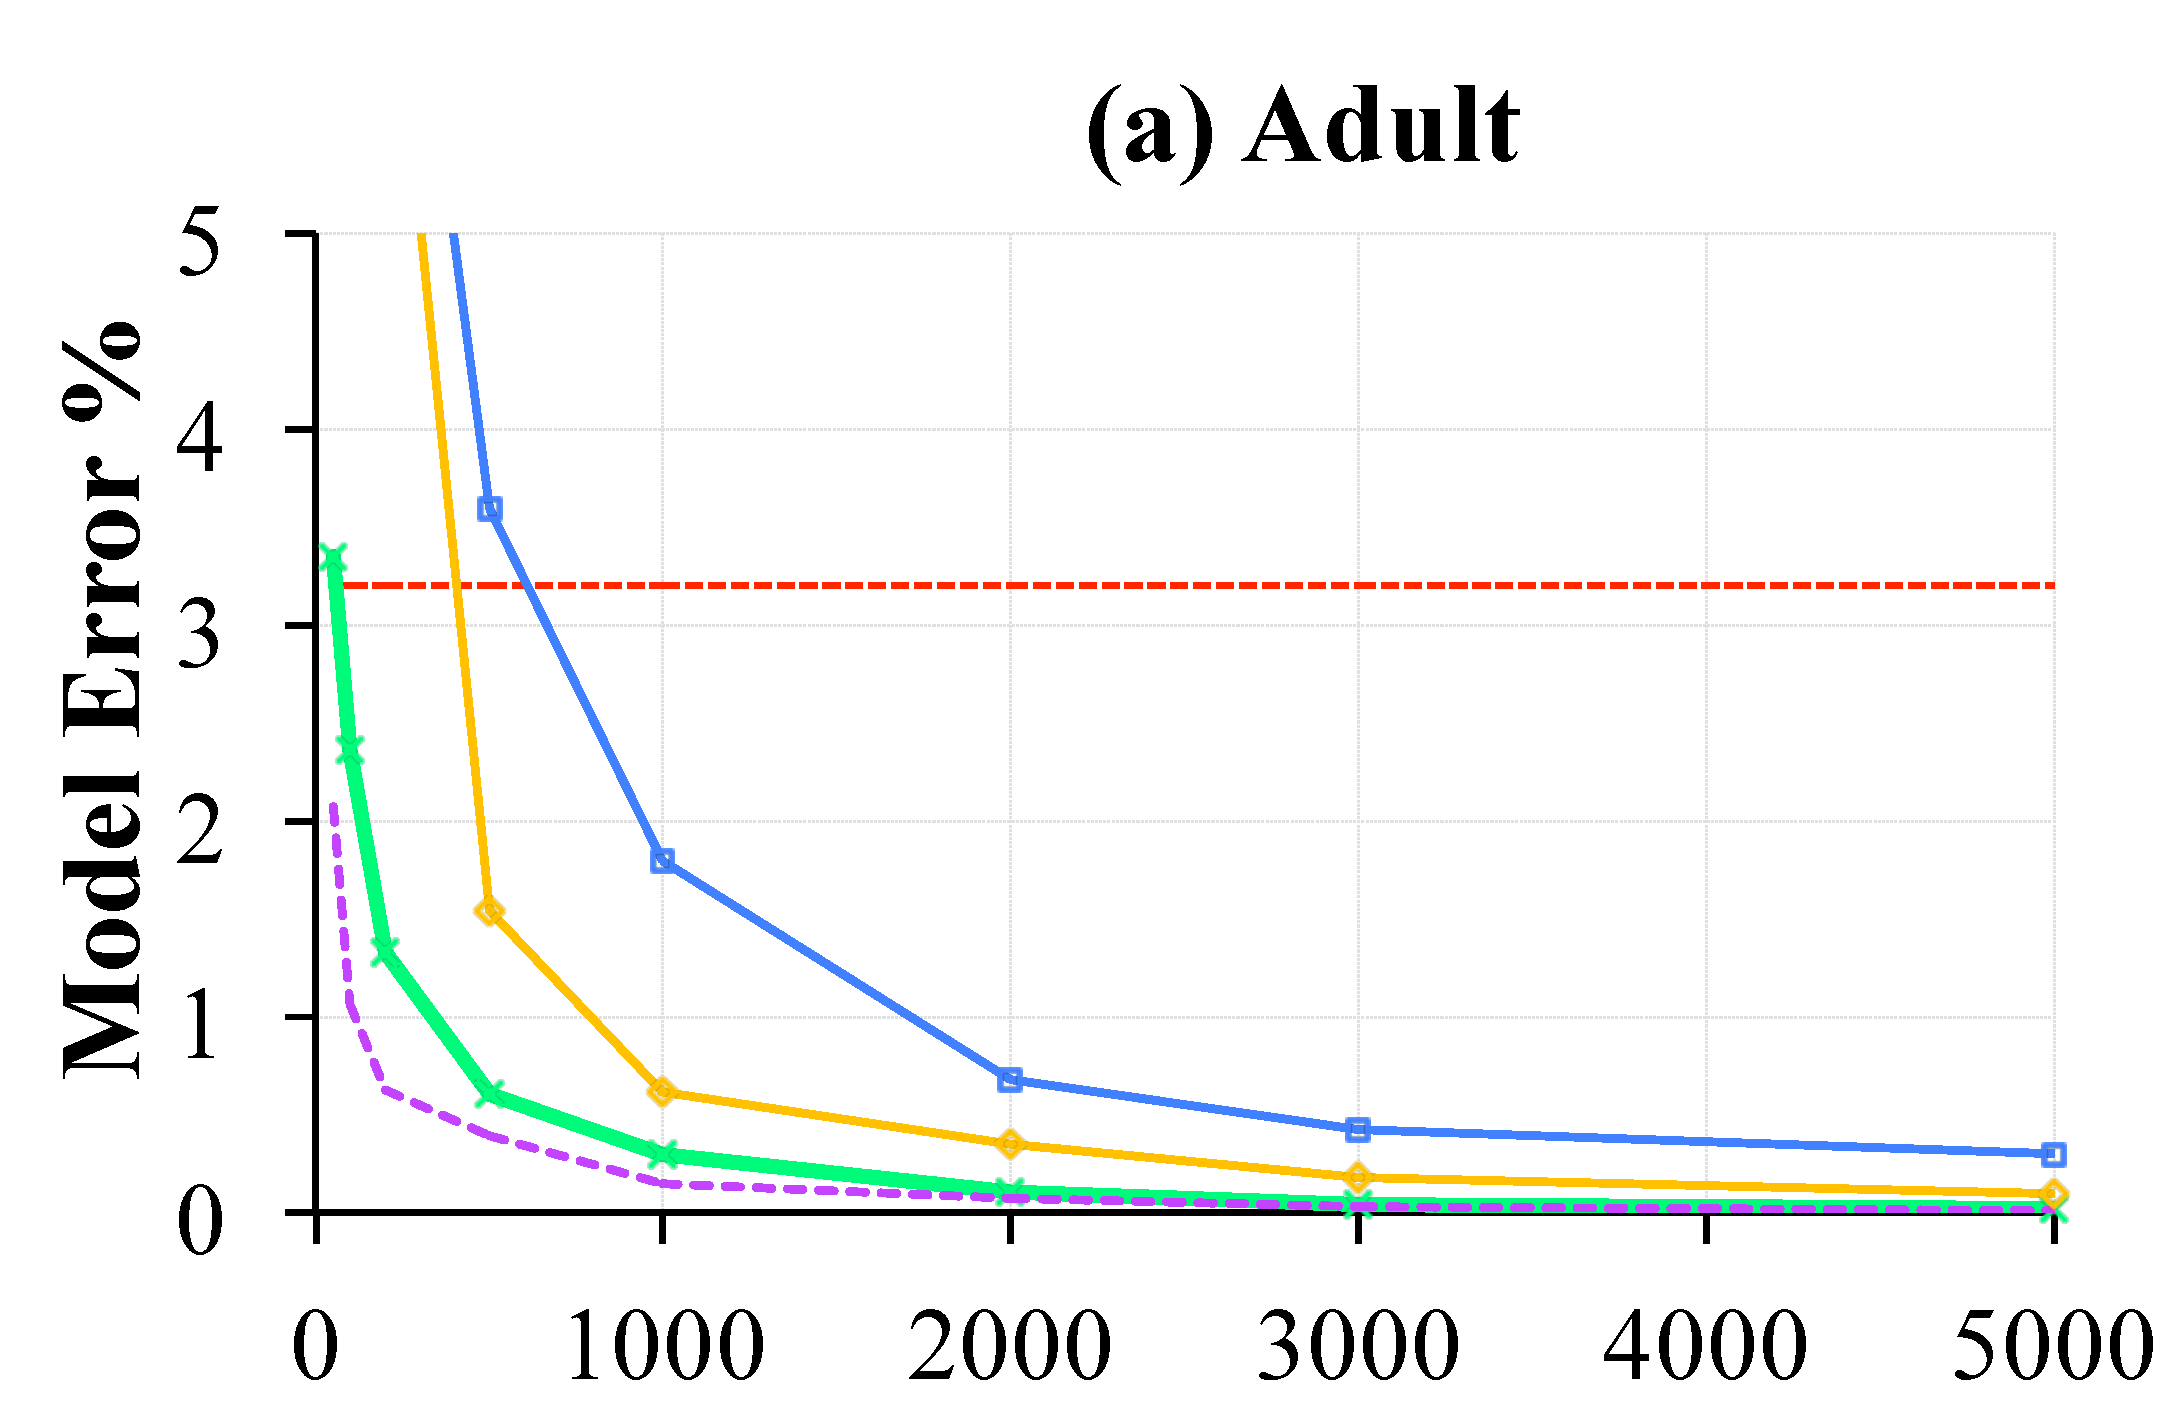
\includegraphics[width=0.49\columnwidth]{exp/exp3b.pdf}
  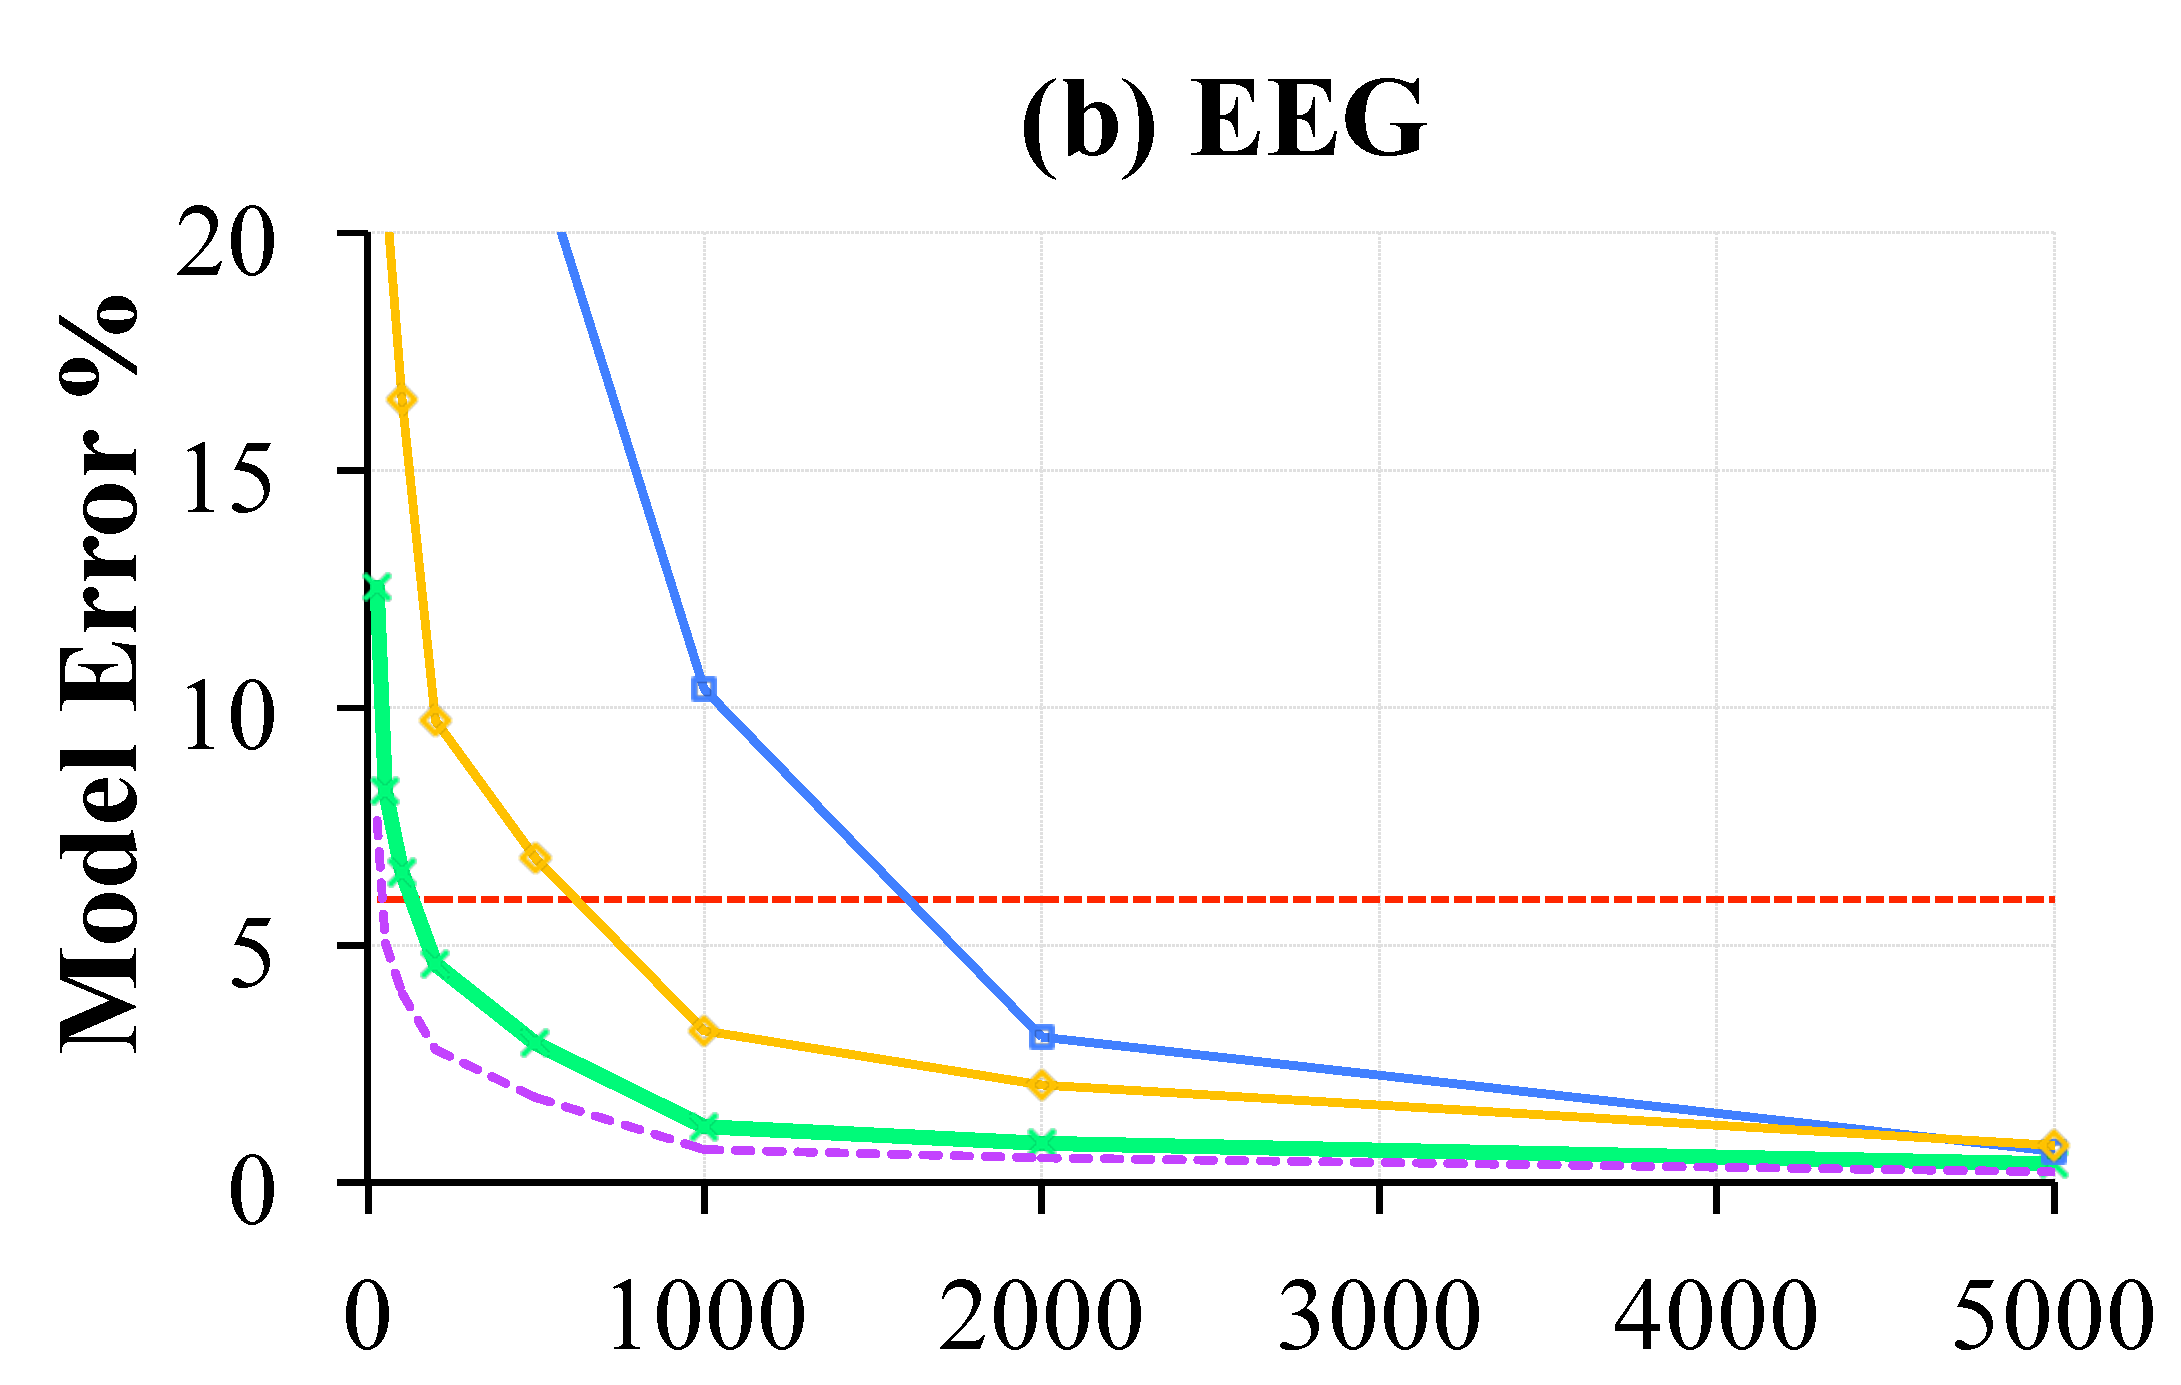
\includegraphics[width=0.49\columnwidth]{exp/exp3c.pdf}
  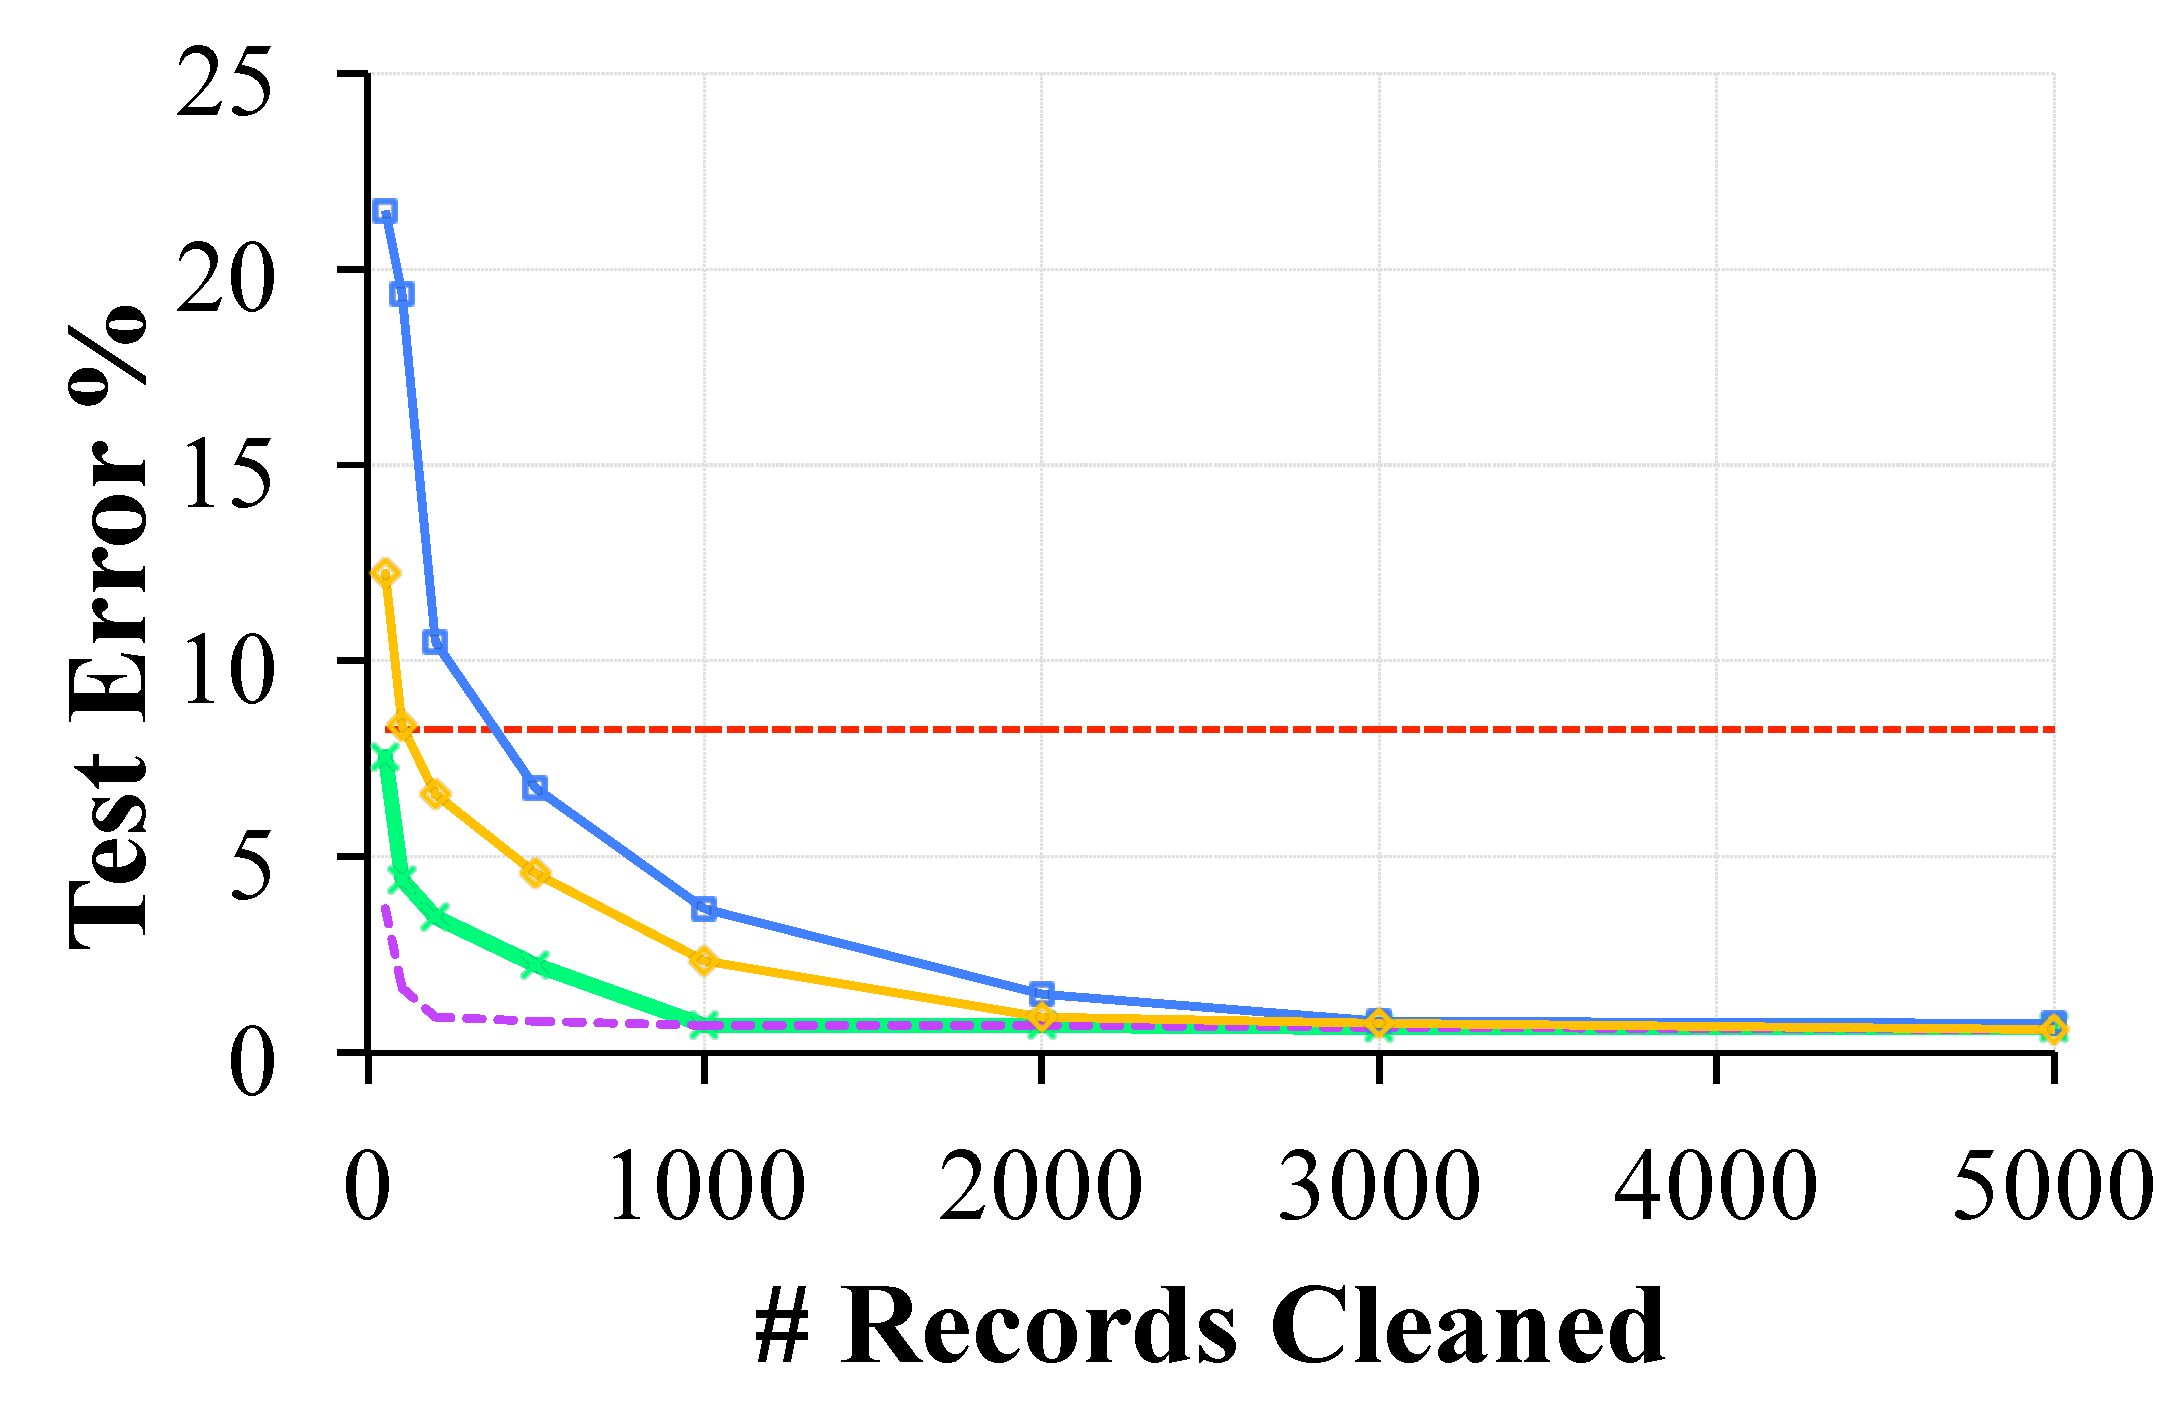
\includegraphics[width=0.49\columnwidth]{exp/exp3bb.pdf}
  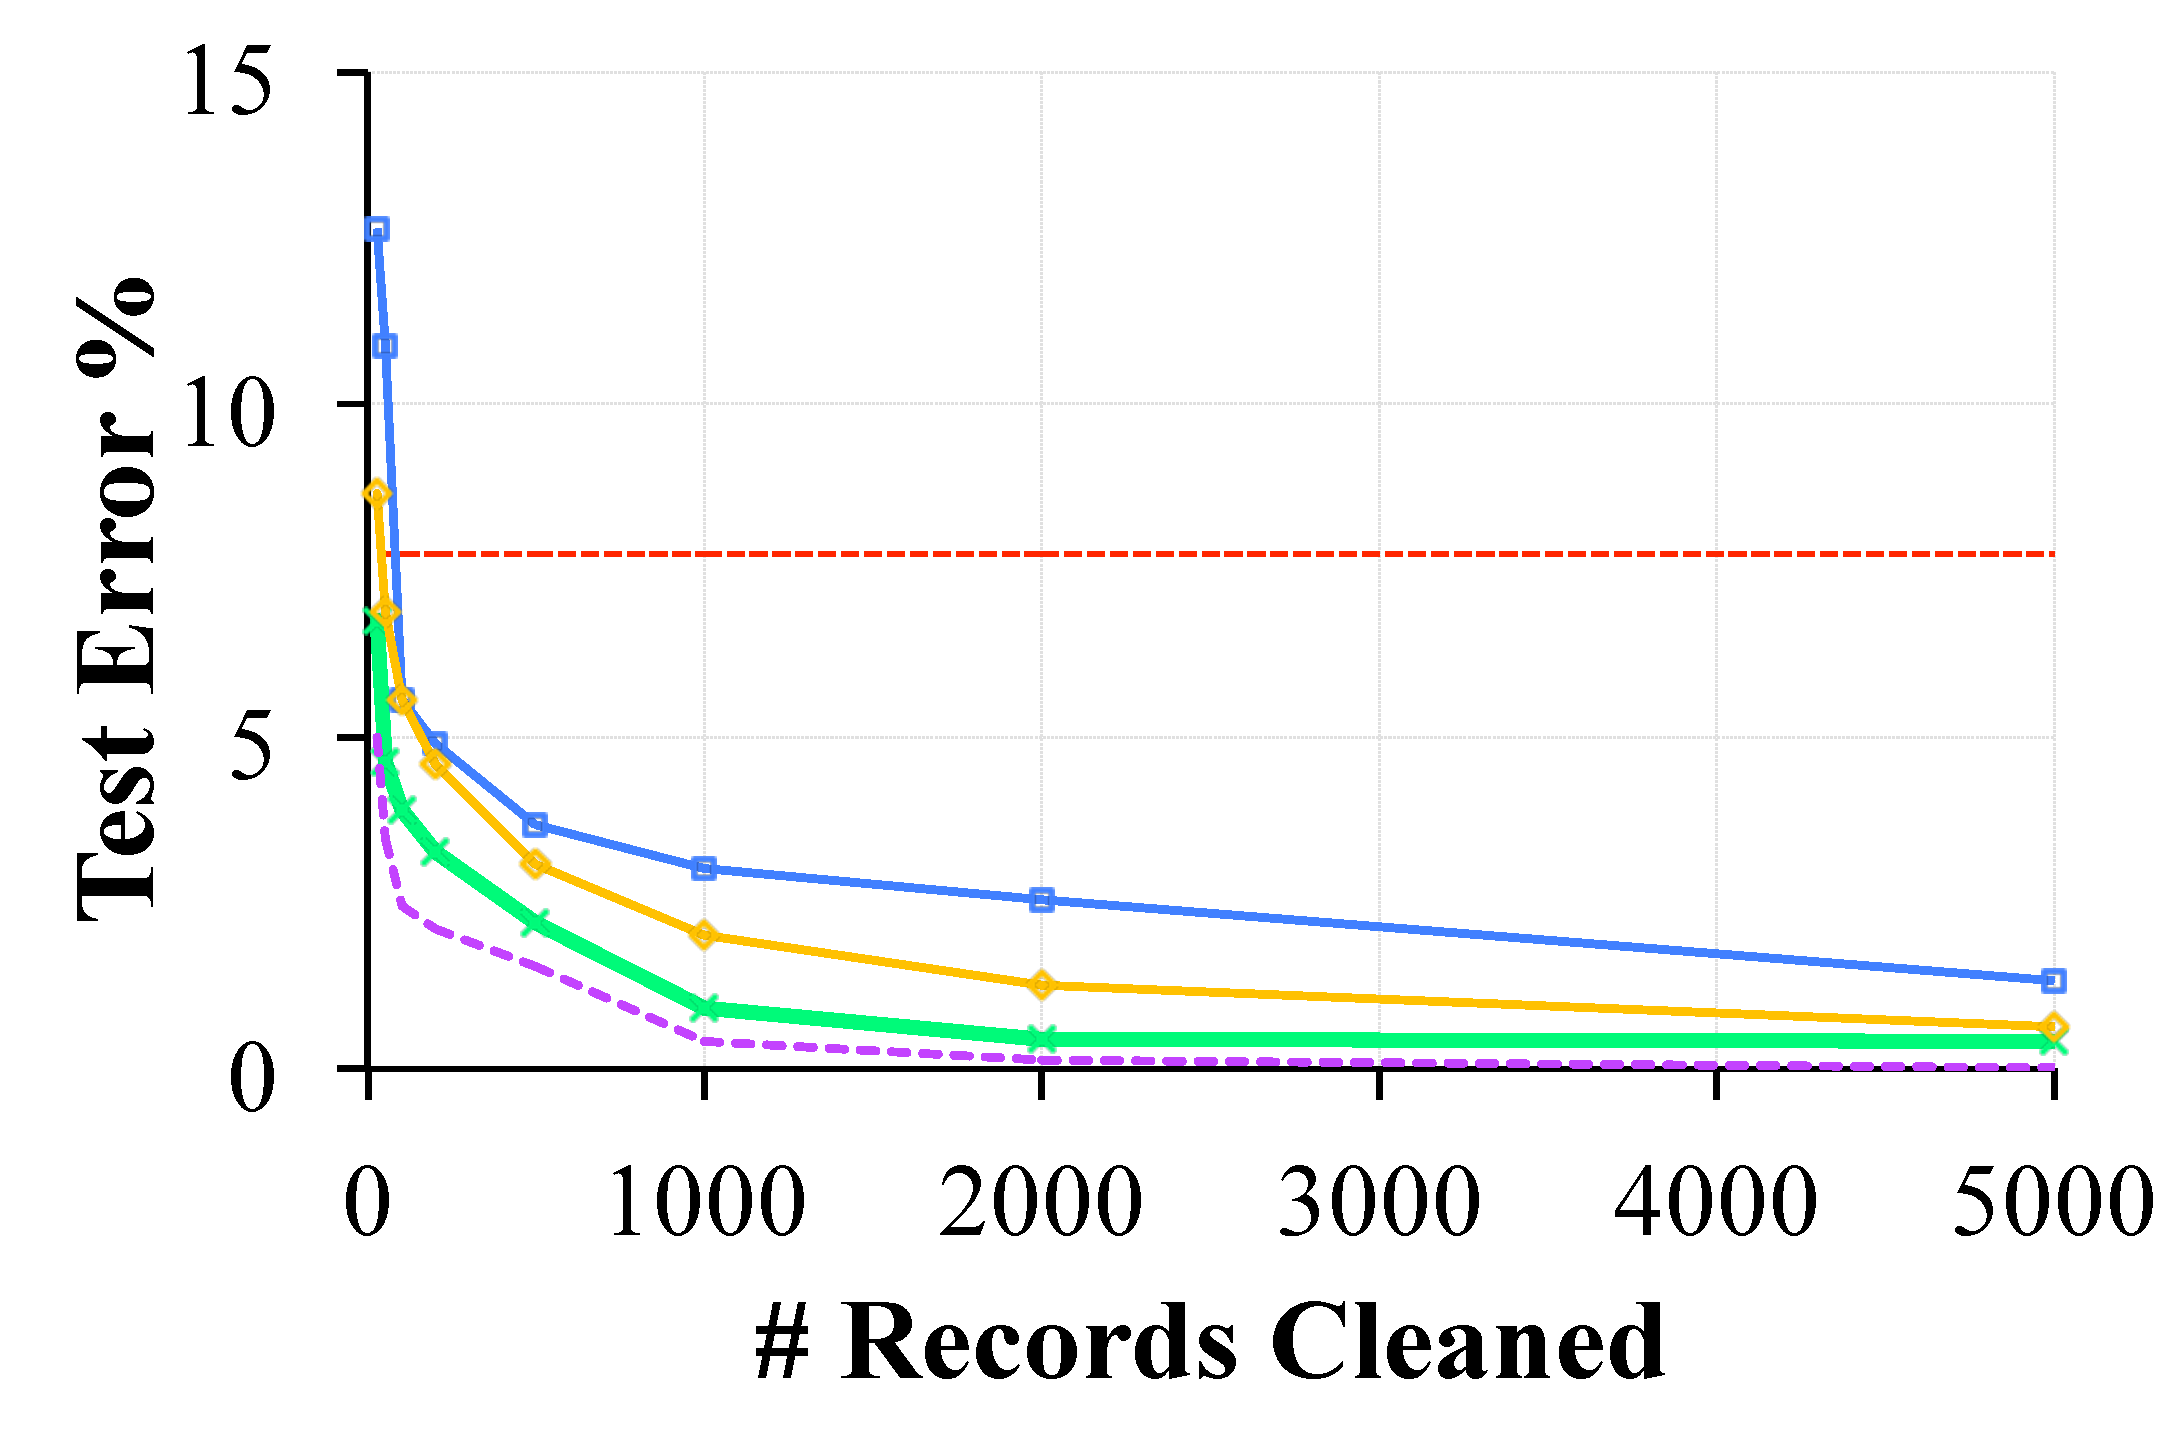
\includegraphics[width=0.49\columnwidth]{exp/exp3cc.pdf}
  
\includegraphics[width=0.5\columnwidth]{exp/legend-general.png}\vspace{-0.5em}
 \caption{ The relative model error as a function of the number of examples cleaned. \sys converges with a smaller sample size to the true result in comparison to Active Learning and SampleClean. \label{prio-perf}}\vspace{-1em}
\end{figure}

\subsubsection{Source of Improvements}\label{comp}
The next experiment compares the performance of \sys with and without various optimizations at 500 records cleaned point. 
This is a vertical slice of the plots in the previous experiments.
\sys without detection is denoted as (AC-D) (that is at each iteration we sample from the entire dirty data), and \sys without detection and importance sampling is denoted as (AC-D-I).
Figure \ref{opts} plots the relative error of the alternatives and \sys with and without the optimizations.
Without detection (AC-D), \sys is still more accurate than Active Learning.
Removing the importance sampling, \sys is slightly worse than Active Learning on the Adult dataset but is comparable on the EEG dataset.

\begin{figure}[t]\vspace{0.5em}
\centering
 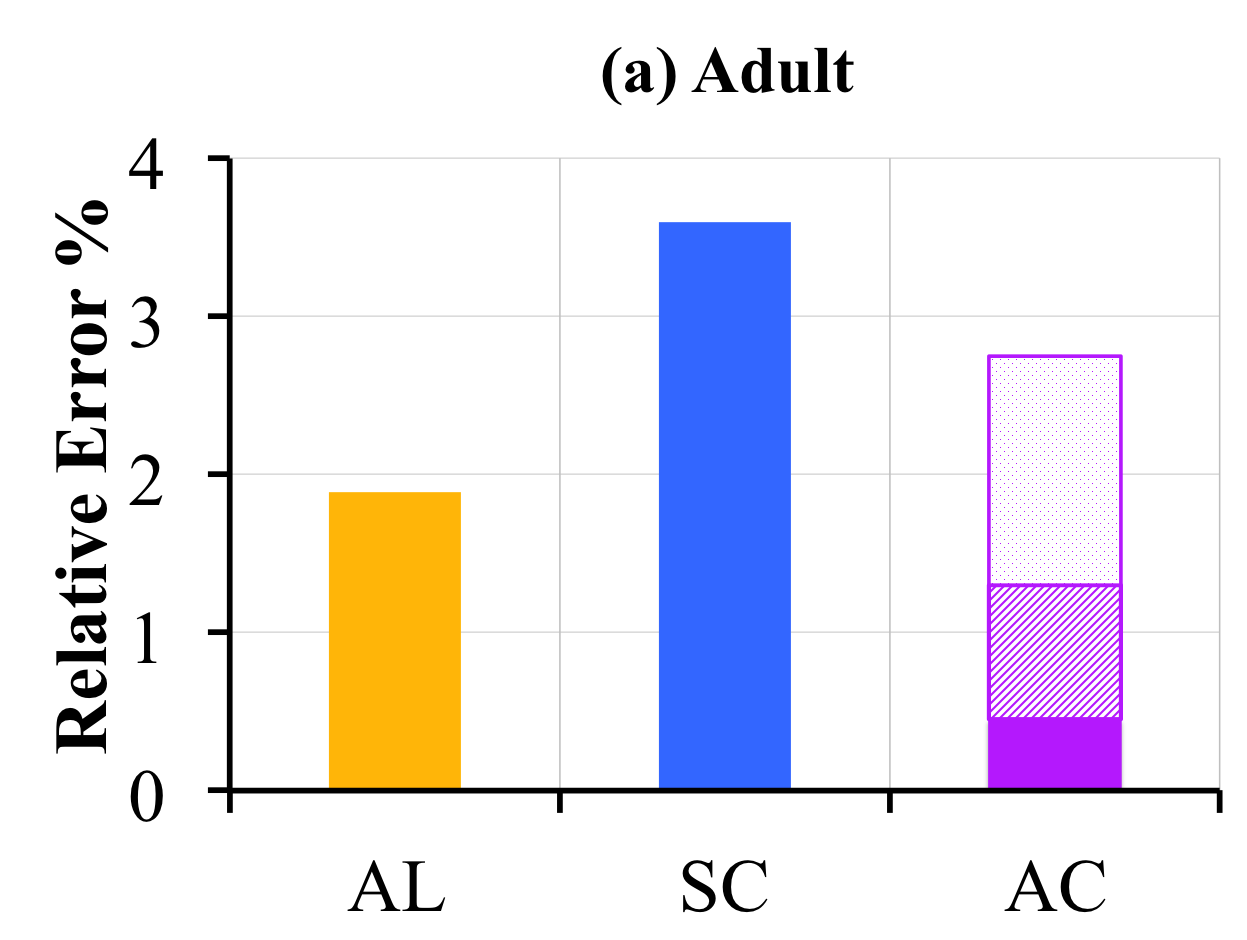
\includegraphics[width=0.49\columnwidth]{exp/exp8a.png}
 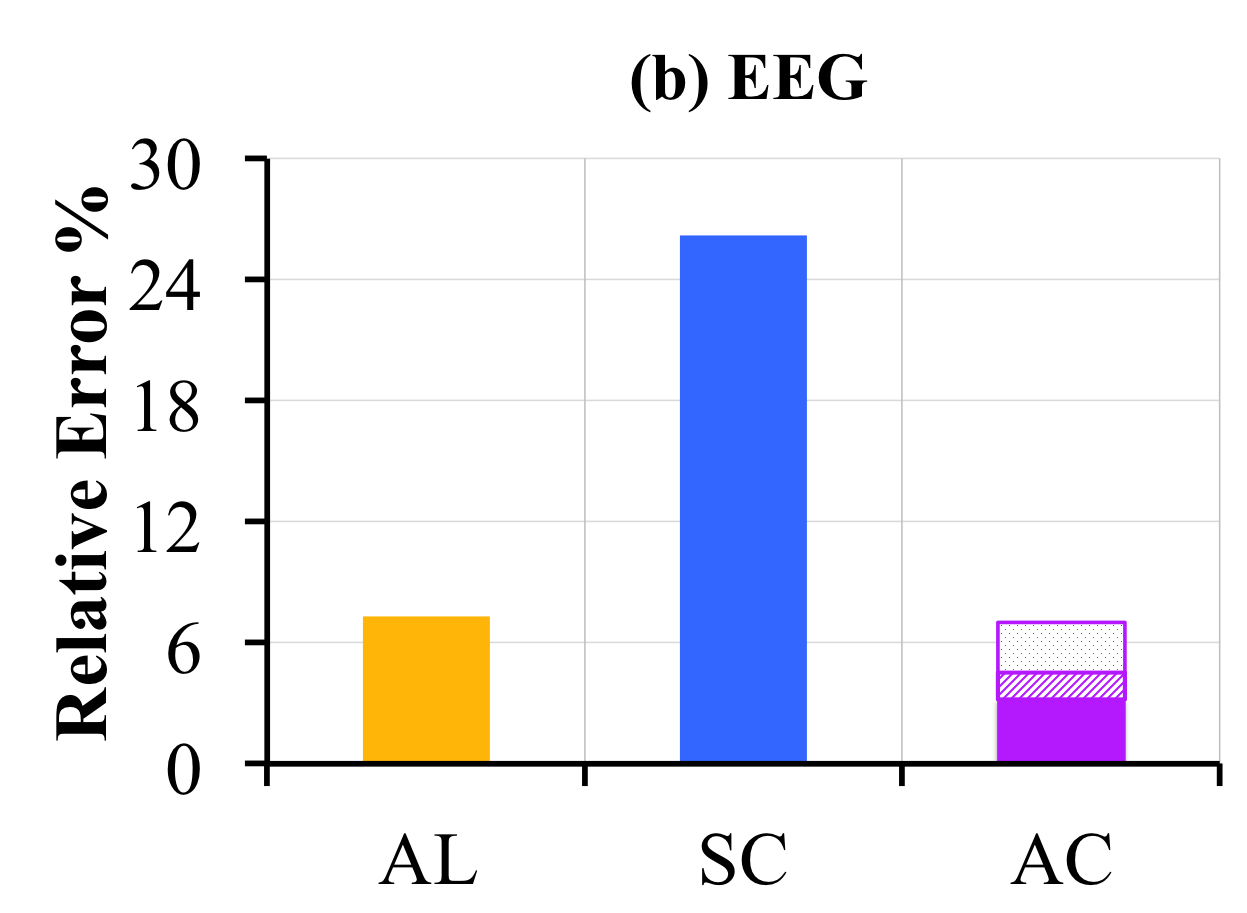
\includegraphics[width=0.49\columnwidth]{exp/exp8b.png}
 
\includegraphics[width=0.5\columnwidth]{exp/legend-8.png}\vspace{-1em}
 \caption{ -D denotes no detection, and -D-I denotes no detection and no importance sampling. Both optimizations significantly help \sys outperform SampleClean and Active Learning. \label{opts}}\vspace{-1.5em}
\end{figure}

\vspace{0.25em}

\noindent \emph{Summary: Both a priori detection and non-uniform sampling significantly contribute to the gains over Active Learning.}

\iffalse
We evaluate Active Learning and \sys to better understand this relationship.
In Figure \ref{albias}, we vary the biasing effect of the random corruptions.
That is, we start with zero mean noise and increase the mean value and variance of the noise.
Since Active Learning uses the gradient, if there is zero mean noise, in expectation, the dirty data and clean data are the same.
However, as the bias increases, the fact that Active Learning prioritizes w.r.t to the dirty data matters more and becomes increasingly erroneous w.r.t to \sys.

\begin{figure}[ht!]
\centering
 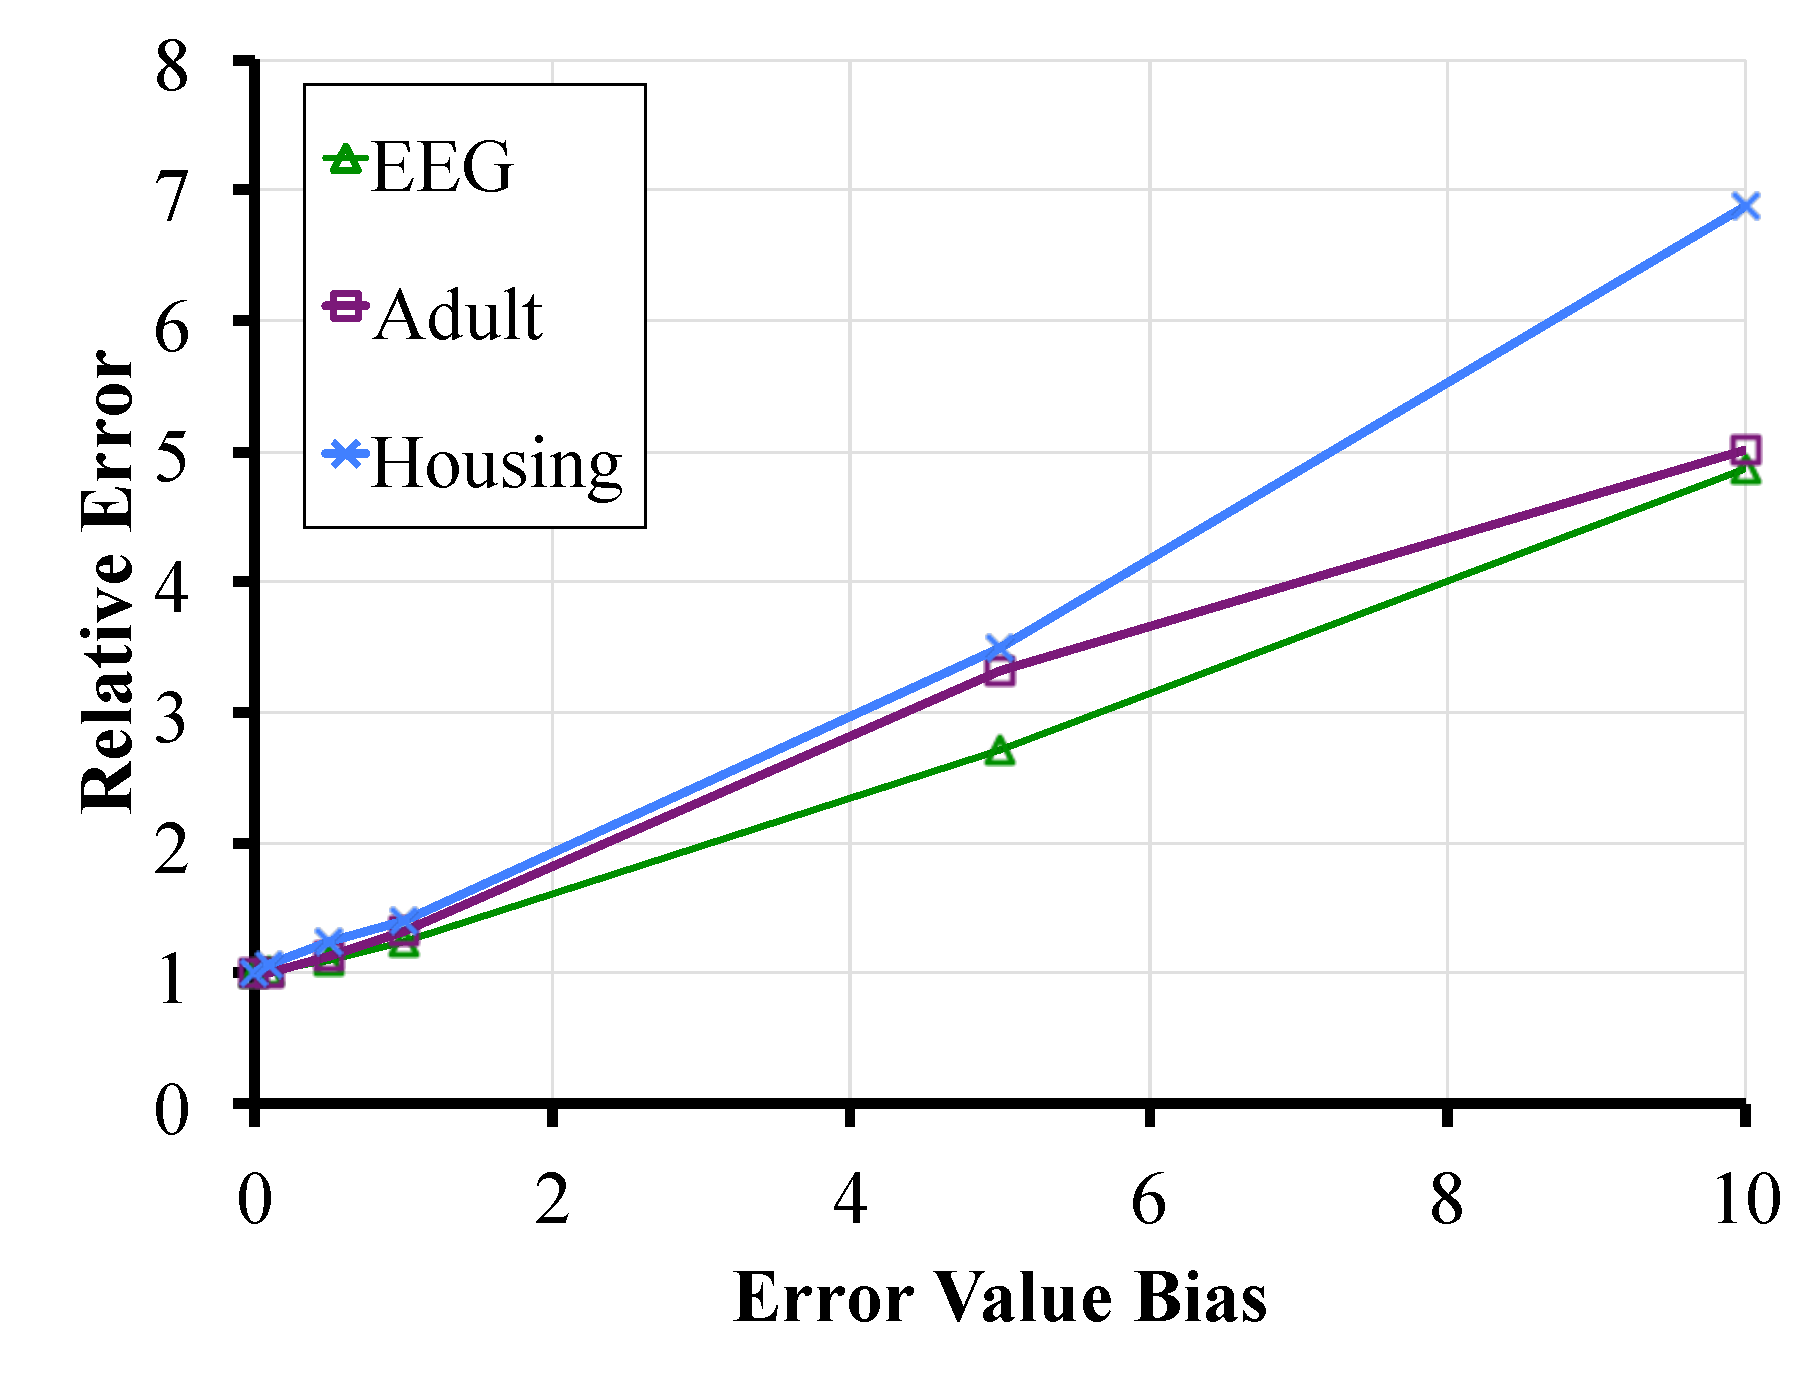
\includegraphics[width=0.6\columnwidth]{exp/exp10.pdf}
 \caption{As we increase the biasing nature of the corruption, Active Learning is increasingly erroneous w.r.t \sys. \label{albias}}
\end{figure}
\fi

\subsubsection{Mixing Dirty and Clean Data}
Training a model on mixed data is an unreliable methodology lacking the same guarantees as Active Learning or SampleClean even in the simplest of cases.
For thoroughness, the next experiments include the model error as a function of records cleaned in comparison to \sys.
Figure \ref{pc-perf} plots the same curves as the previous experiment comparing \sys, Active Learning, and two mixed data algorithms.
PC randomly samples data, clean, and writes-back the cleaned data.
PC+D randomly samples data from using the dirty data detector, cleans, and writes-back the cleaned data.
For these errors PC and PC+D give reasonable results (not always guaranteed), but \sys converges faster.
This is because \sys tunes the weighting when averaging dirty and clean data into the gradient.

\begin{figure}[ht!]
\centering\vspace{-0.5em}
 %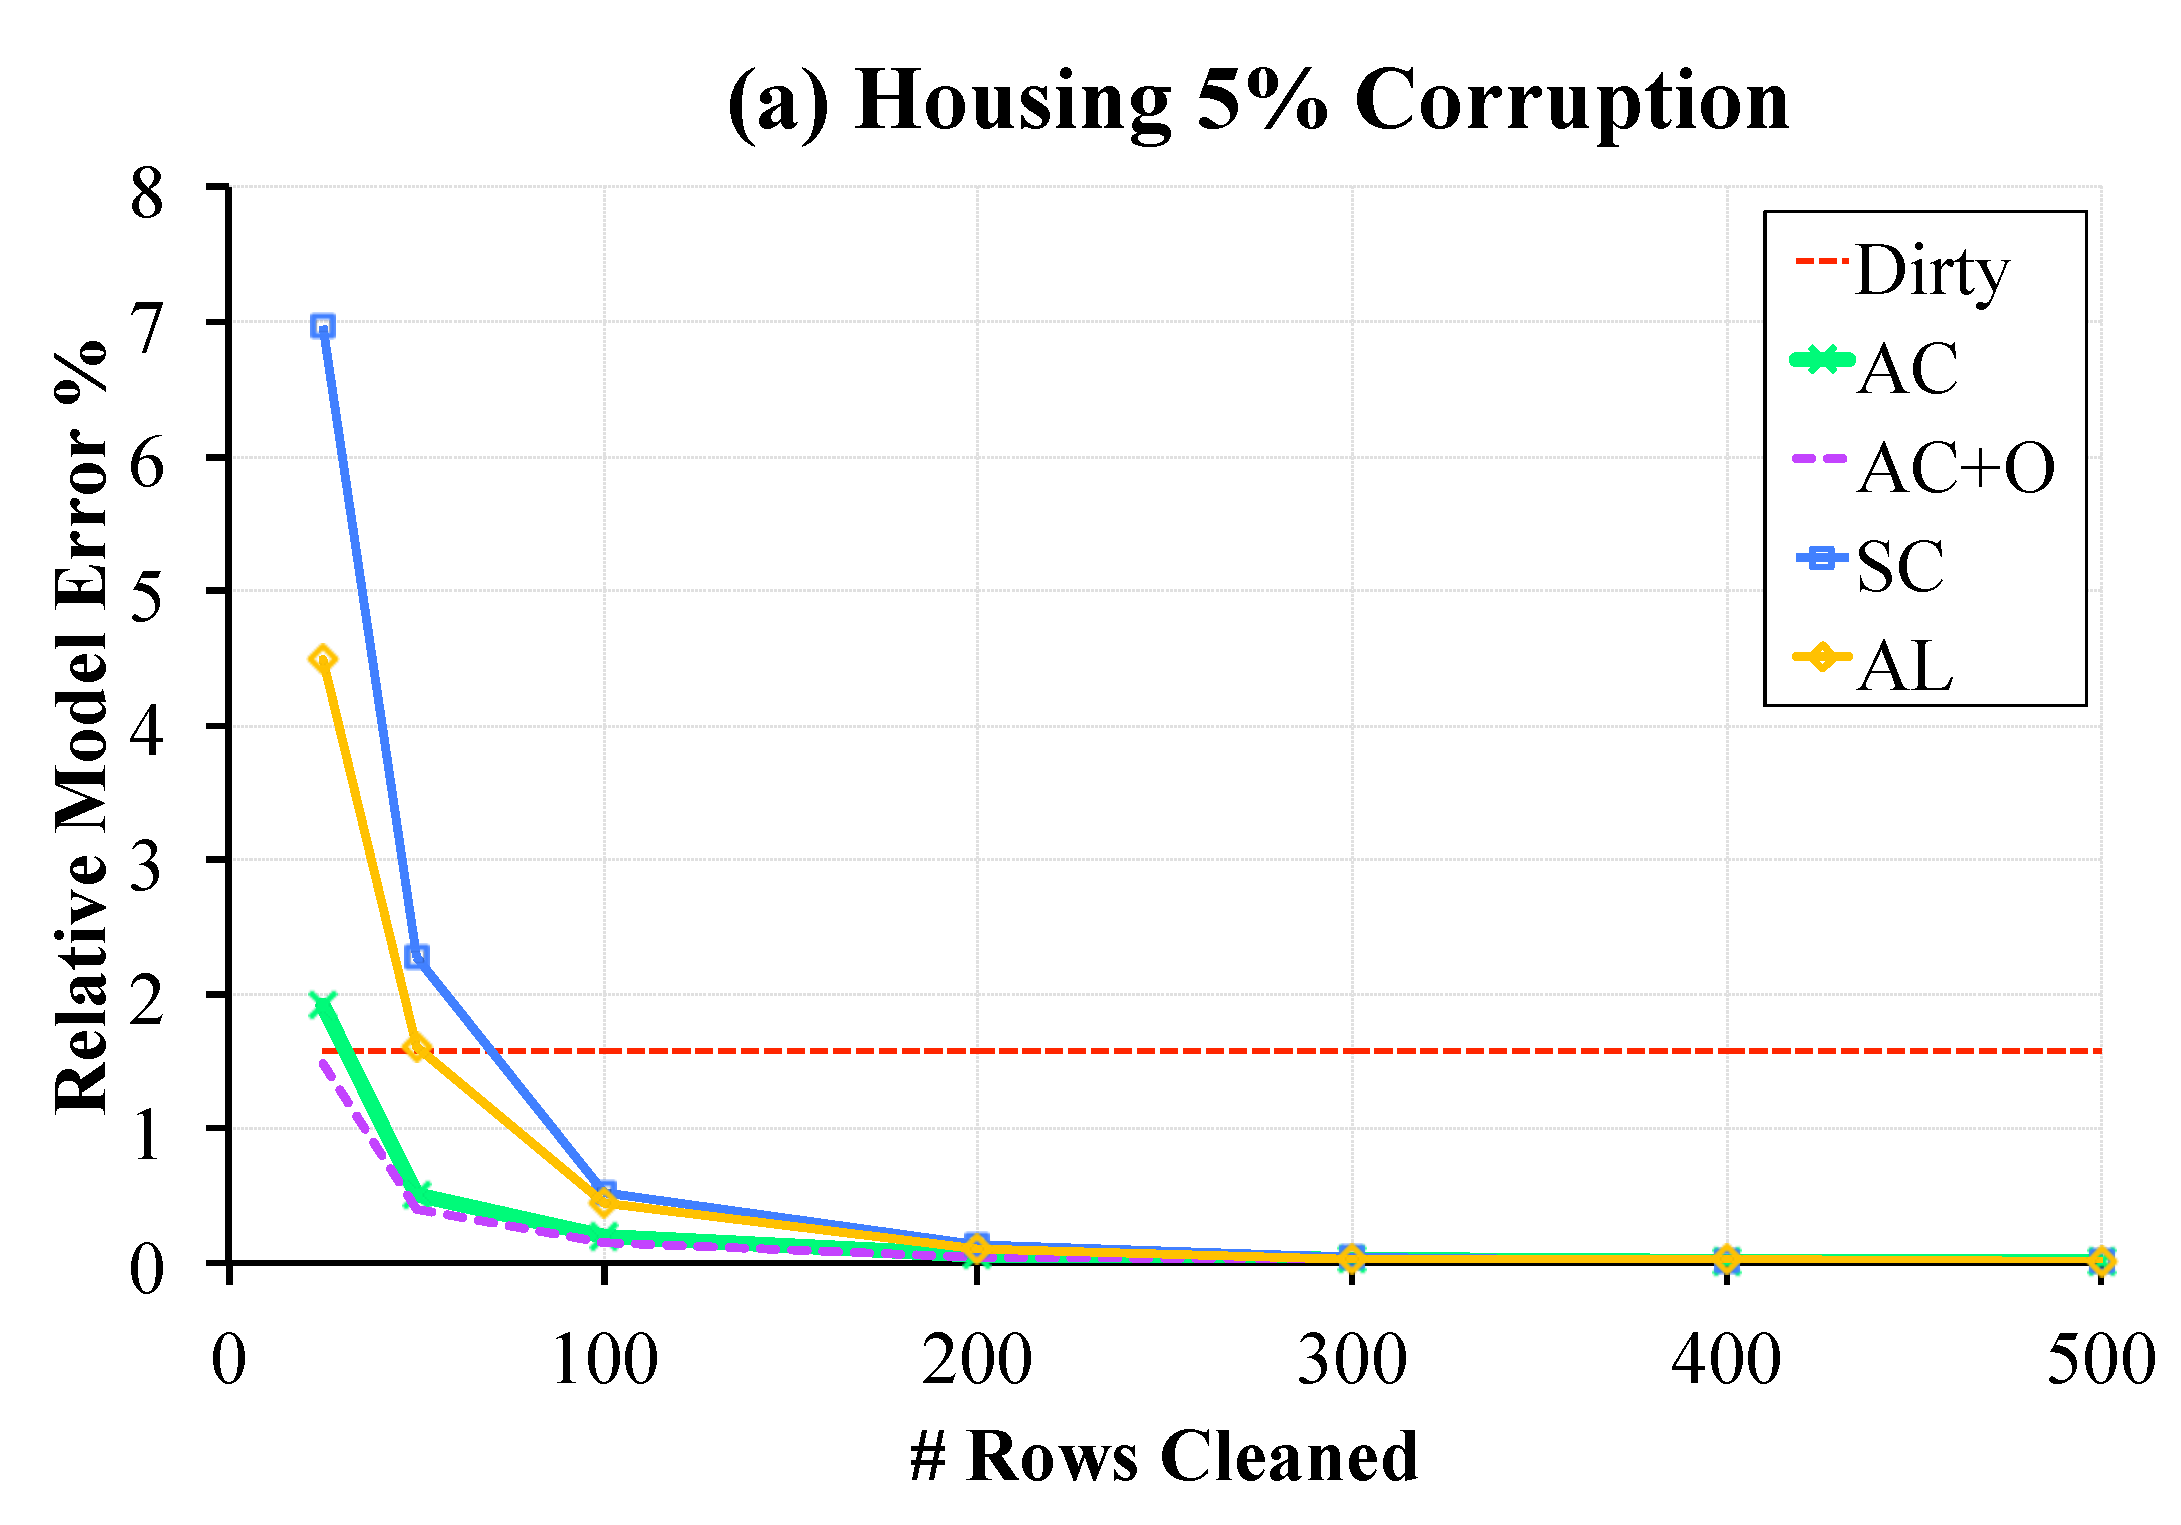
\includegraphics[scale=0.15]{exp/exp3a.pdf}
 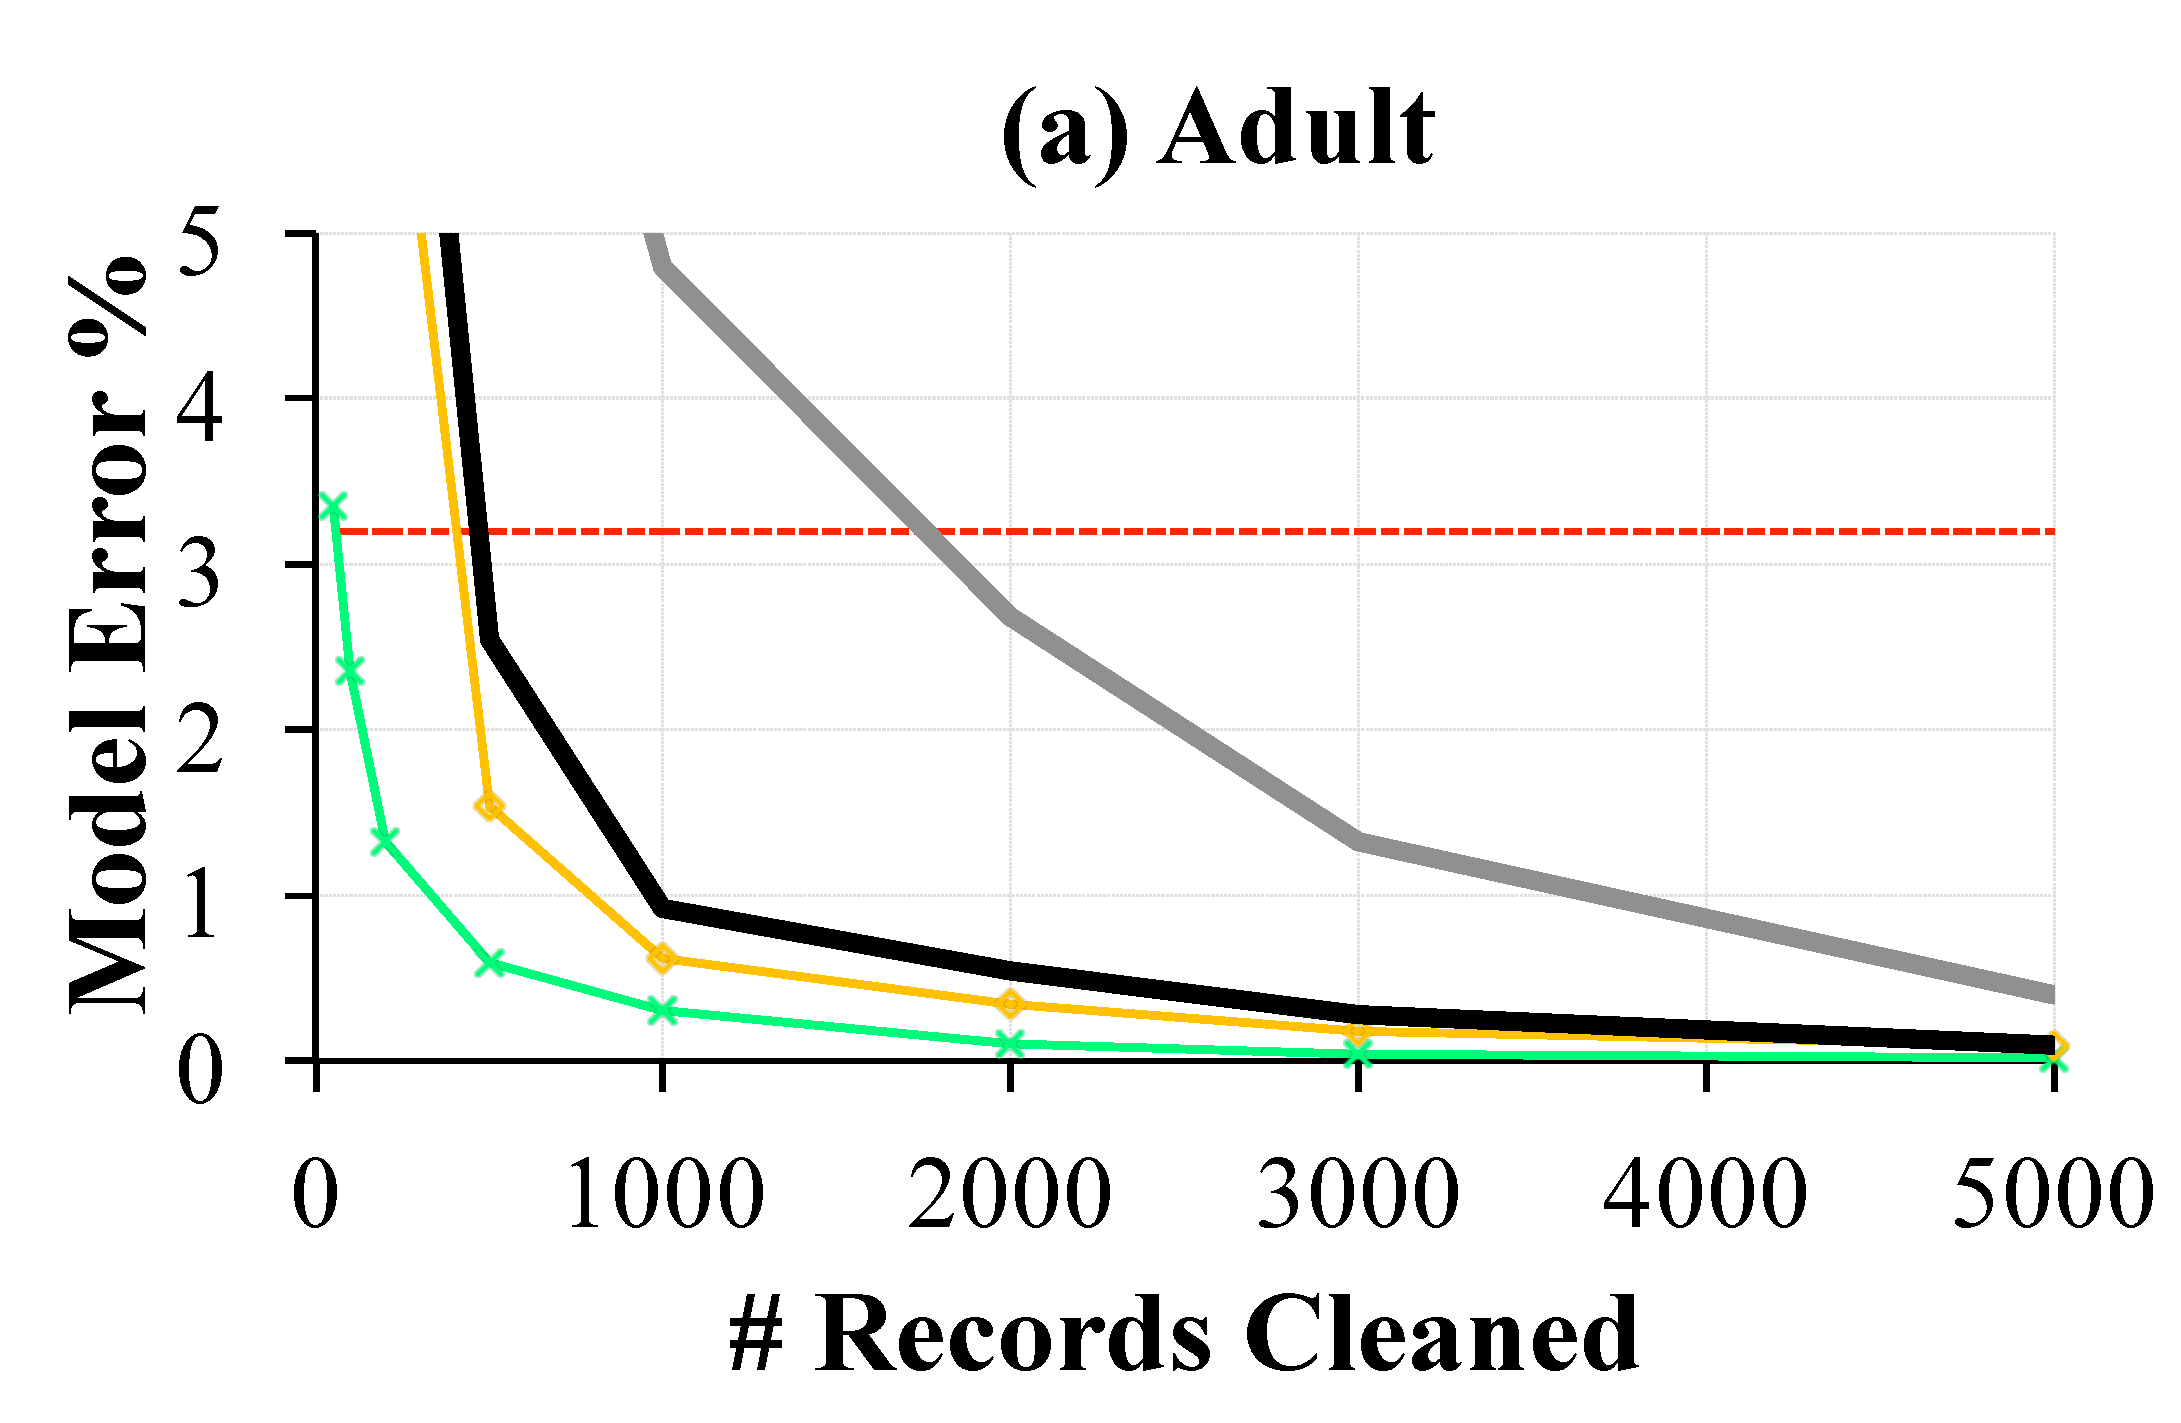
\includegraphics[width=0.49\columnwidth]{exp/exp14a.pdf}
    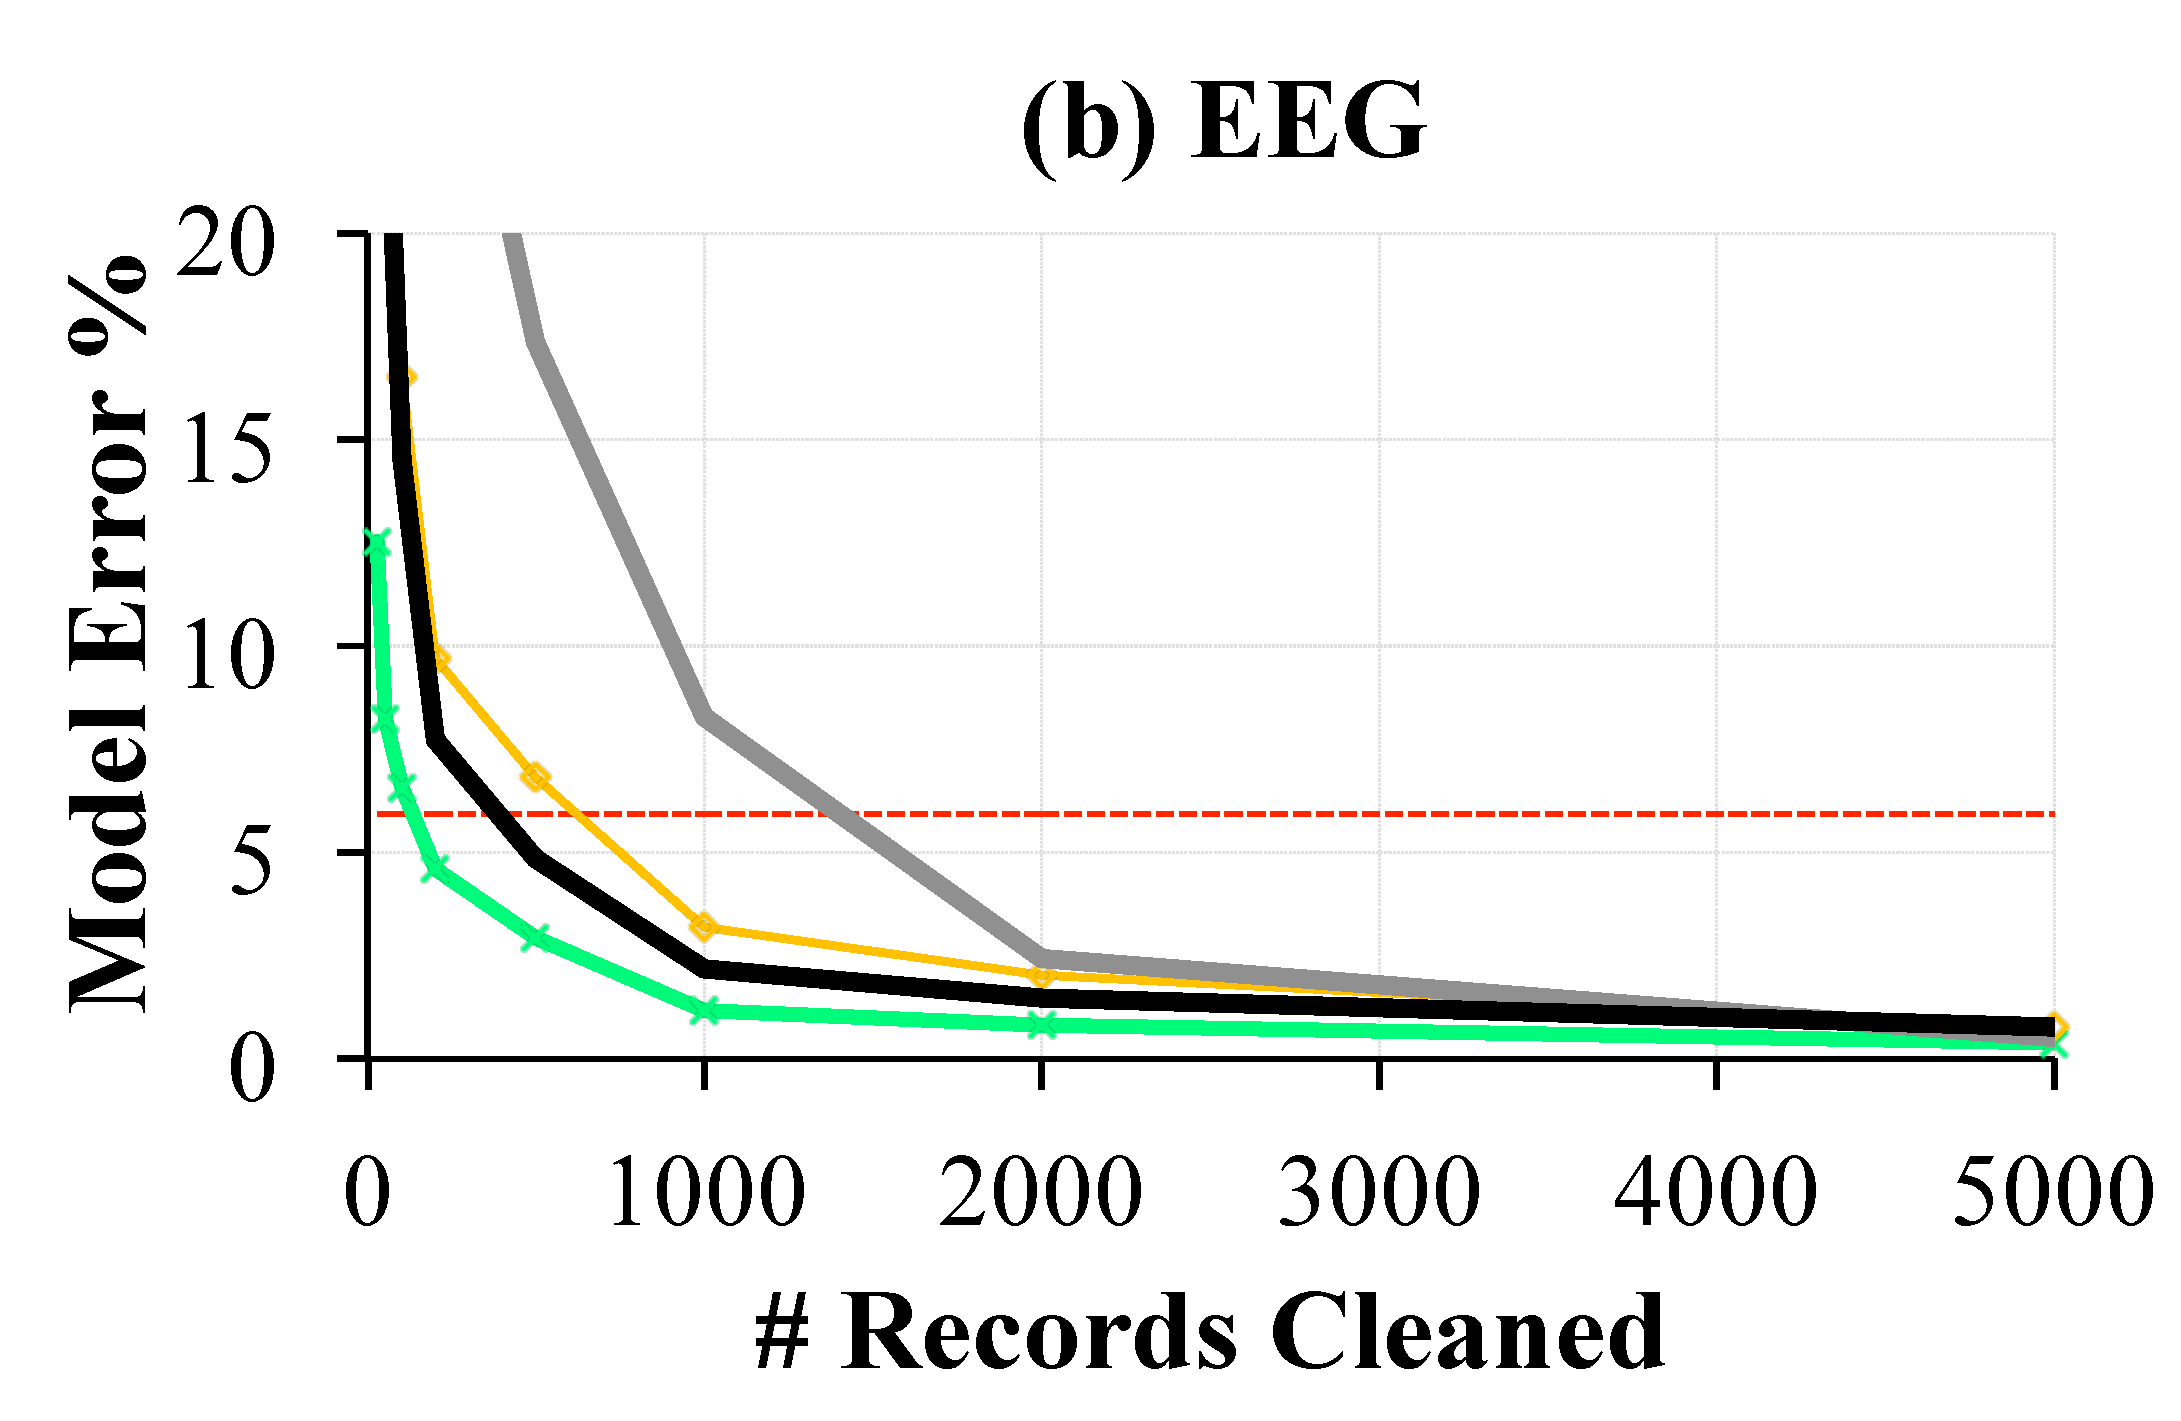
\includegraphics[width=0.49\columnwidth]{exp/exp14b.pdf}
    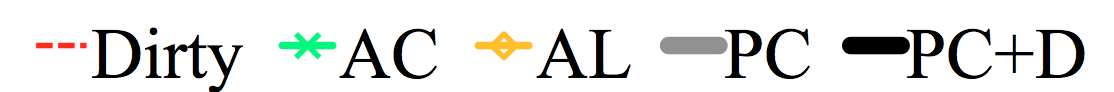
\includegraphics[width=0.49\columnwidth]{exp/legend-14.png}\vspace{-0.5em}
 \caption{The relative model error as a function of the number of examples cleaned. \sys converges with a smaller sample size to the true result in comparison to partial cleaning (PC,PC+D).  \label{pc-perf}}
\end{figure}

\noindent \emph{Summary: \sys converges faster than mixing dirty and clean data since it reweights data based on the fraction that is dirty and clean. Partial cleaning is not guaranteed to give sensible results.}

\vspace{1em}

\subsubsection{Corruption Rate}
The next experiment explores how much of the performance
is due to the initialization with the dirty model (i.e., SampleClean trains a model from ``scratch").
Figure \ref{bias} varies the systematic corruption rate and plots the number of records cleaned to achieve 1\% relative error for SampleClean and \sys.
SampleClean does not use the dirty data and thus its error is essentially governed by the Central Limit Theorem.
SampleClean outperforms \sys only when corruptions are very severe (45\% in Adult and nearly 60\% in EEG).
When the initialization with the dirty model is inaccurate, \sys does not perform as well. 

\begin{figure}[t]
\centering
 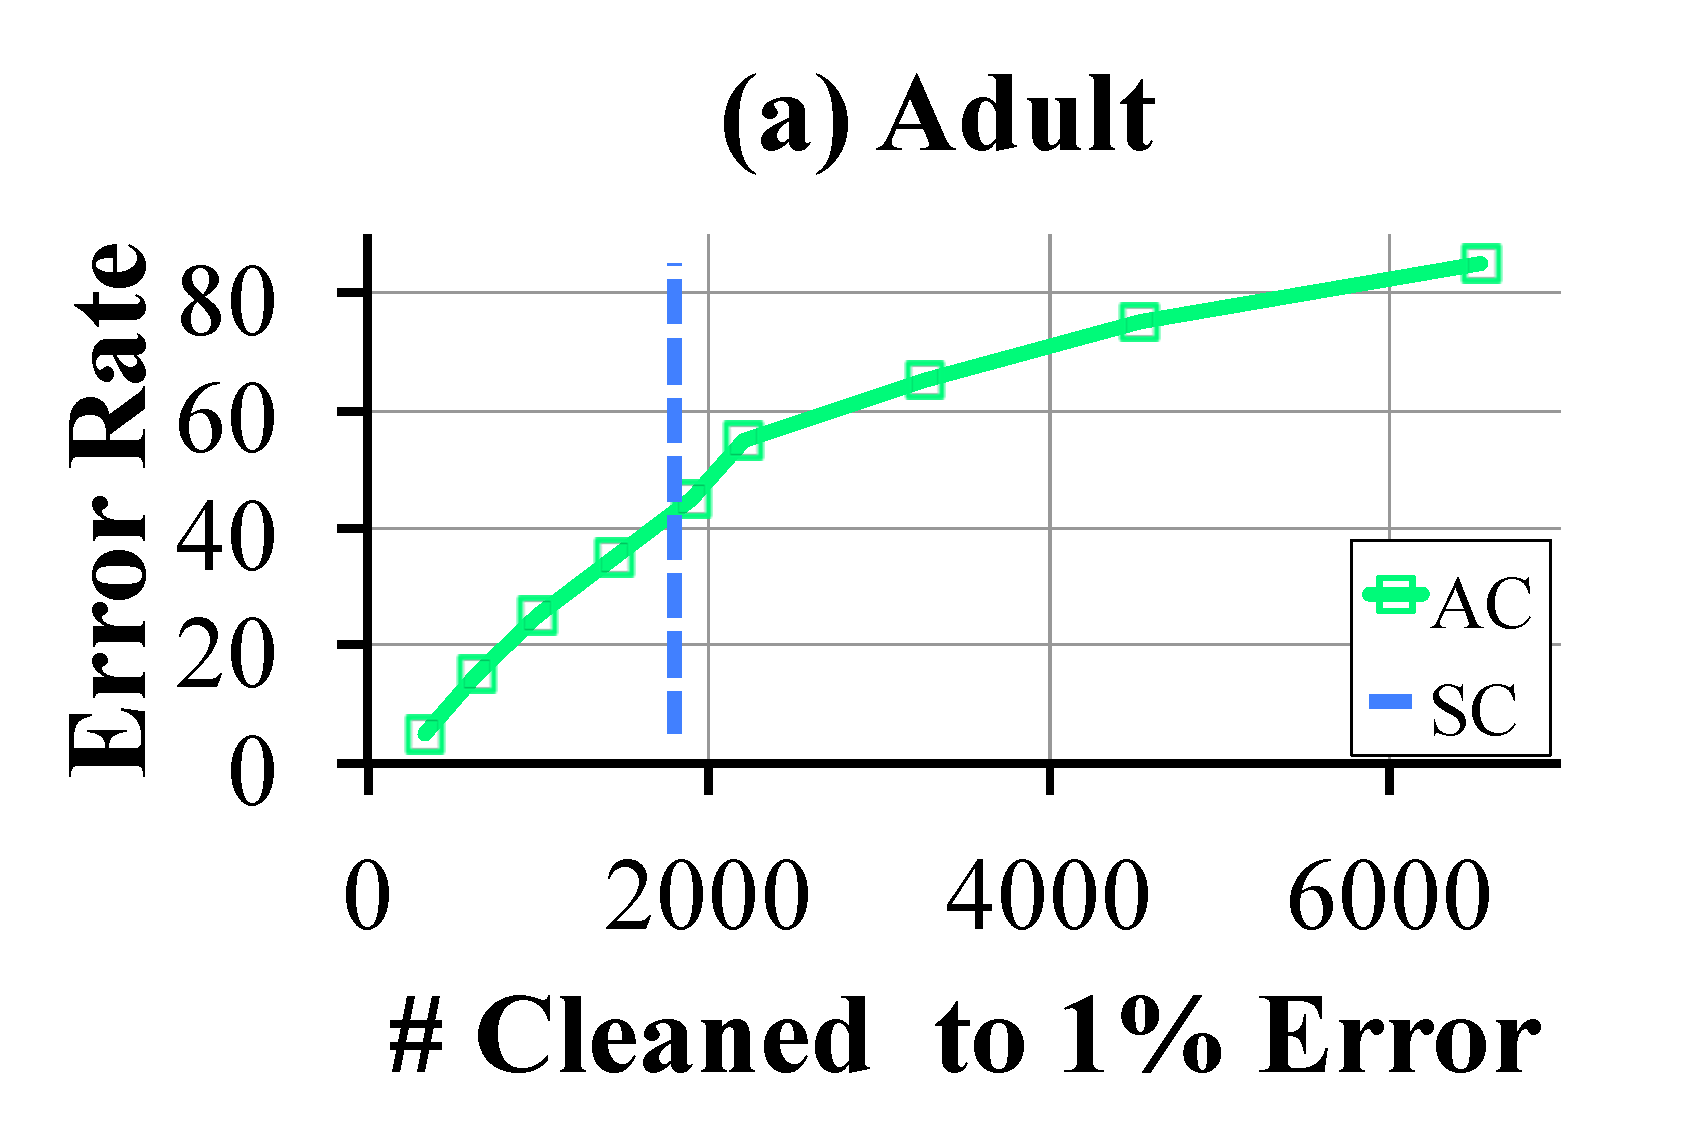
\includegraphics[width=0.49\columnwidth]{exp/exp9a.pdf}
  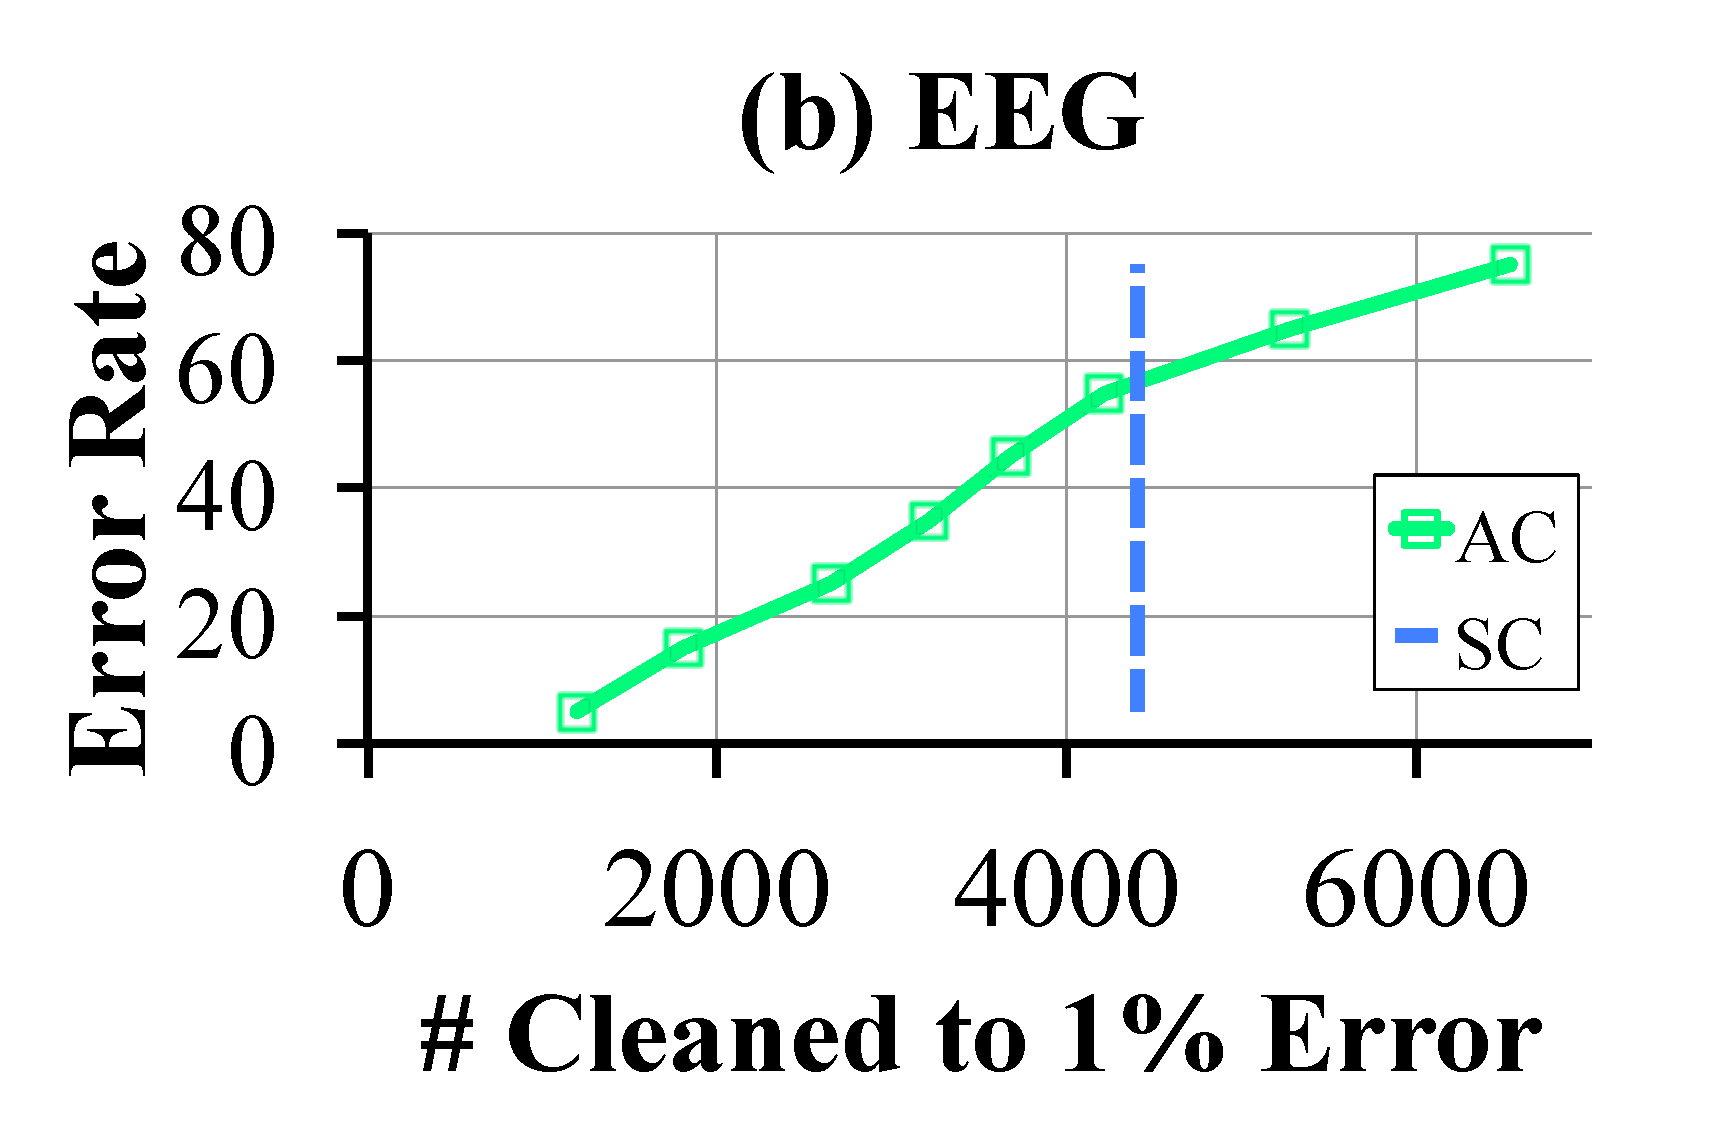
\includegraphics[width=0.49\columnwidth]{exp/exp9b.pdf}\vspace{-1em}
 \caption{\sys performs well until the corruption is so severe that the dirty model is not a good initialization. The error of SampleClean does not depend on the corruption rate so it is a vertical line.  \label{bias}}\vspace{-1.5em}
\end{figure}

\vspace{0.25em}

\noindent \emph{Summary: SampleClean is beneficial in comparison to \sys when corruption rates exceed 45\%.}

\subsection{\sys: Adaptive Detection}
This experiment explores how the results of the previous experiment change when using an adaptive detector instead of the \emph{a priori} detector.
Recall, in the systematic corruption, 3 of the most informative features were corrupted, thus we group these problems into $9$ classes.
We use an all-versus-one SVM to learn the categorization.

\subsubsection{Basic Performance}
Figure \ref{pred-perf} overlays the convergence plots in the previous experiments with a curve (denoted by AC+C) that represents \sys using a classifier instead of the \emph{a priori} detection. Initially \sys is comparable to Active Learning; however, as the classifier becomes more effective the detection improves the performance.
Over both datasets, at the 500 records point on the curve, adaptive \sys has a 30\% higher model error compared to \emph{a priori} \sys.
At 1000 records point on the curve, adaptive \sys has about 10\% higher error.

\vspace{0.25em}

\noindent \emph{Summary: For 500 records cleaned, adaptive \sys has a 30\% higher model error compared to a priori \sys, but still outperforms Active Learning and SampleClean.}

\begin{figure}[ht!]
\centering
 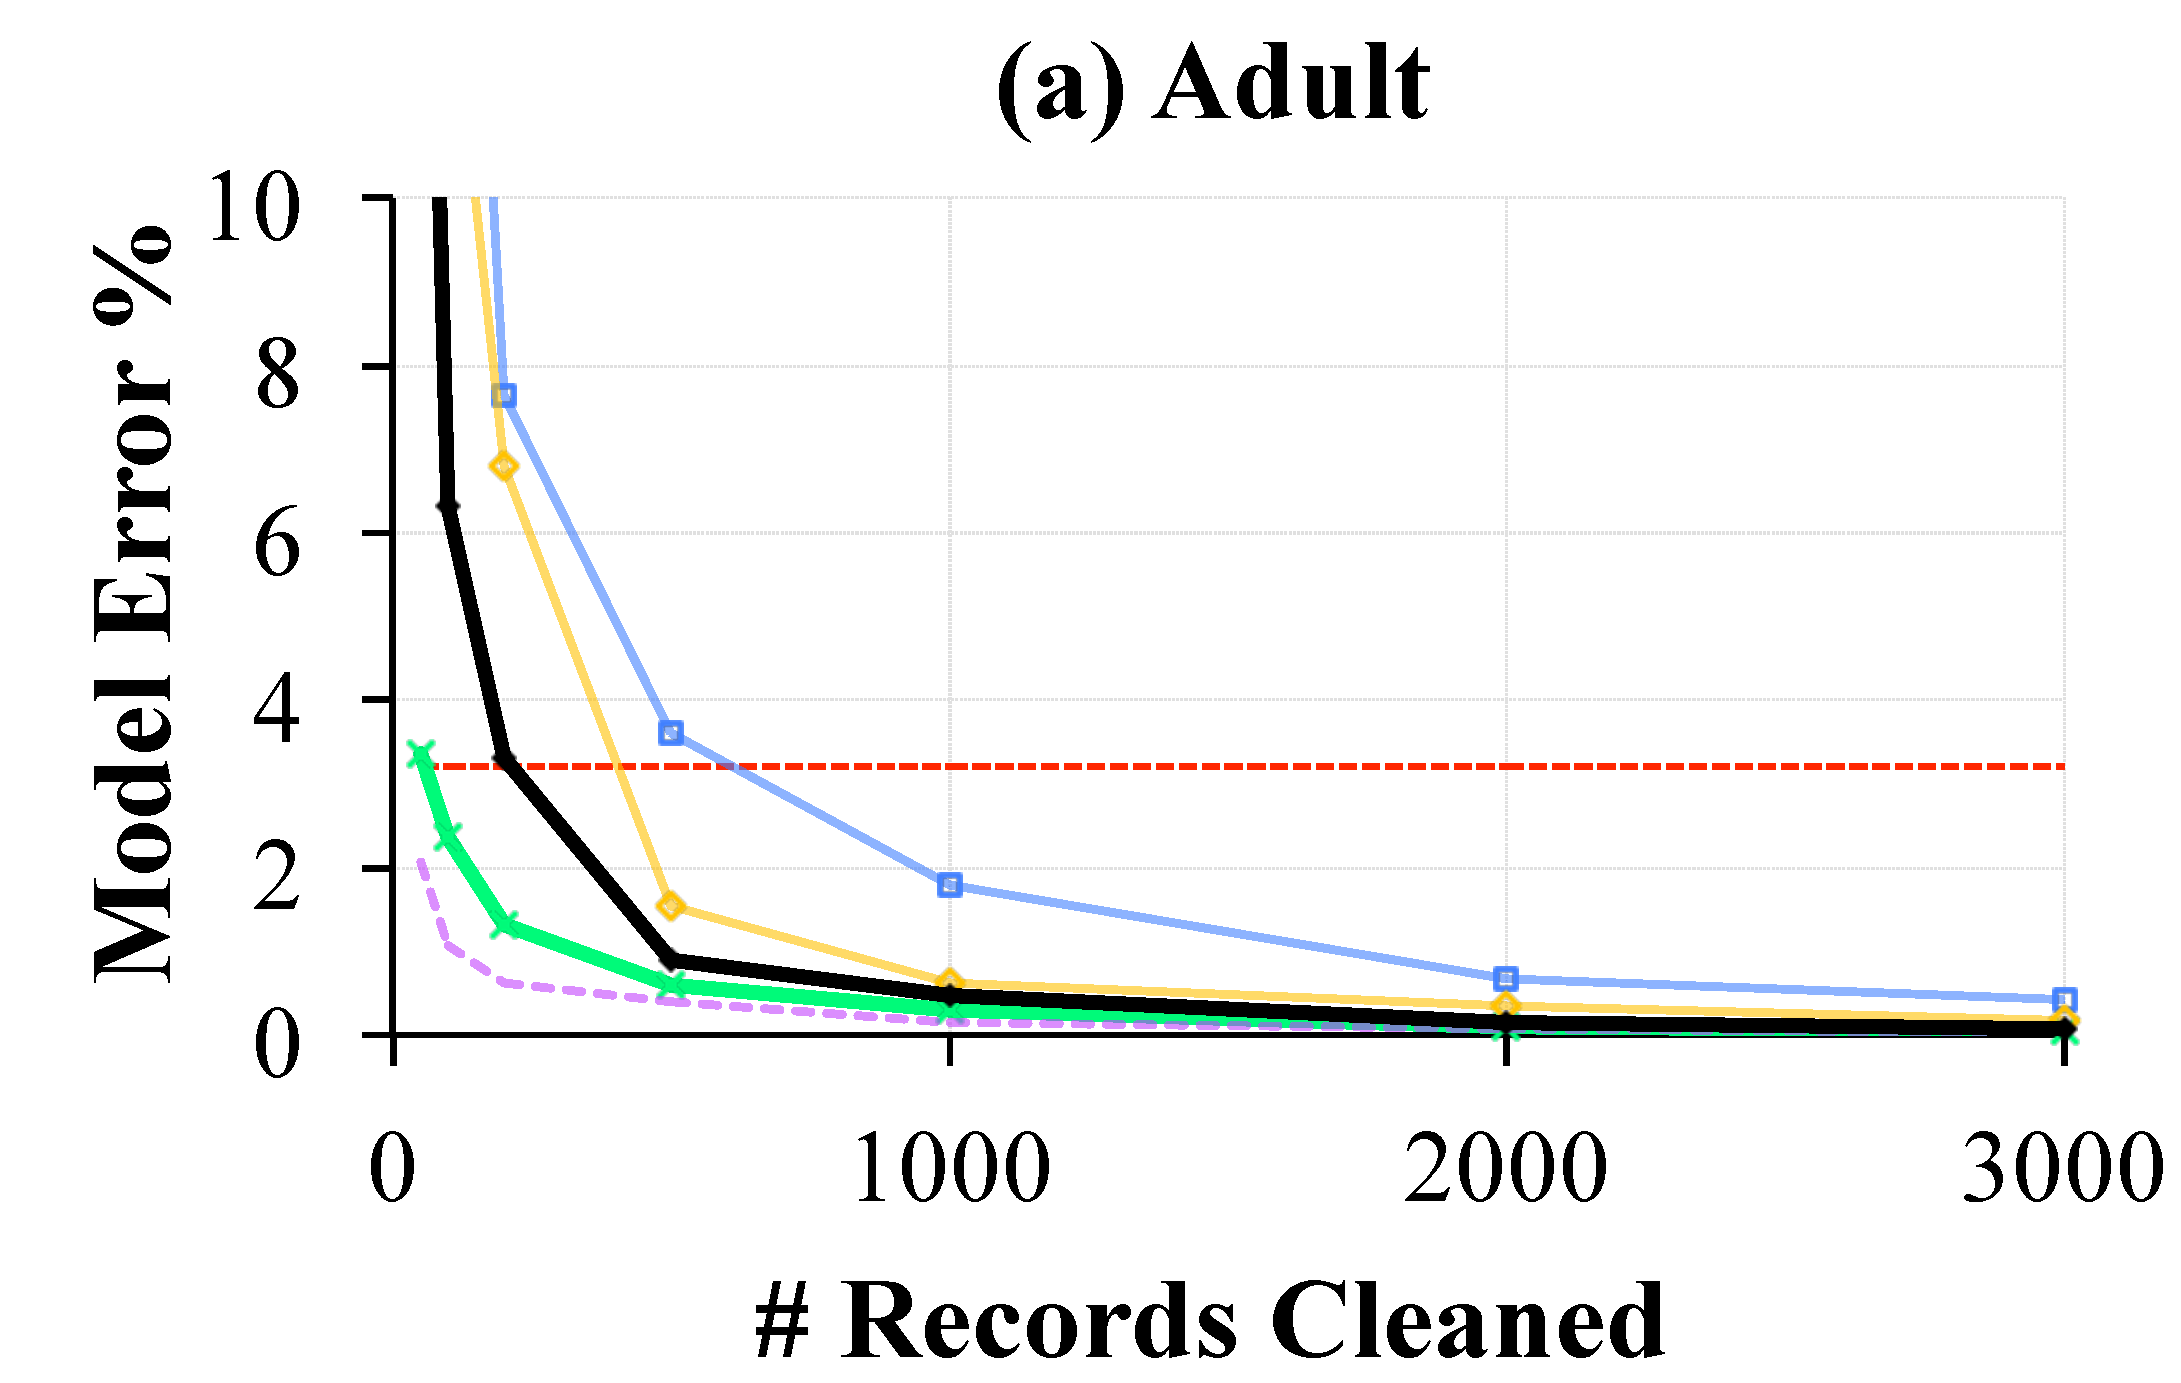
\includegraphics[width=0.49\columnwidth]{exp/exp11a.pdf}
 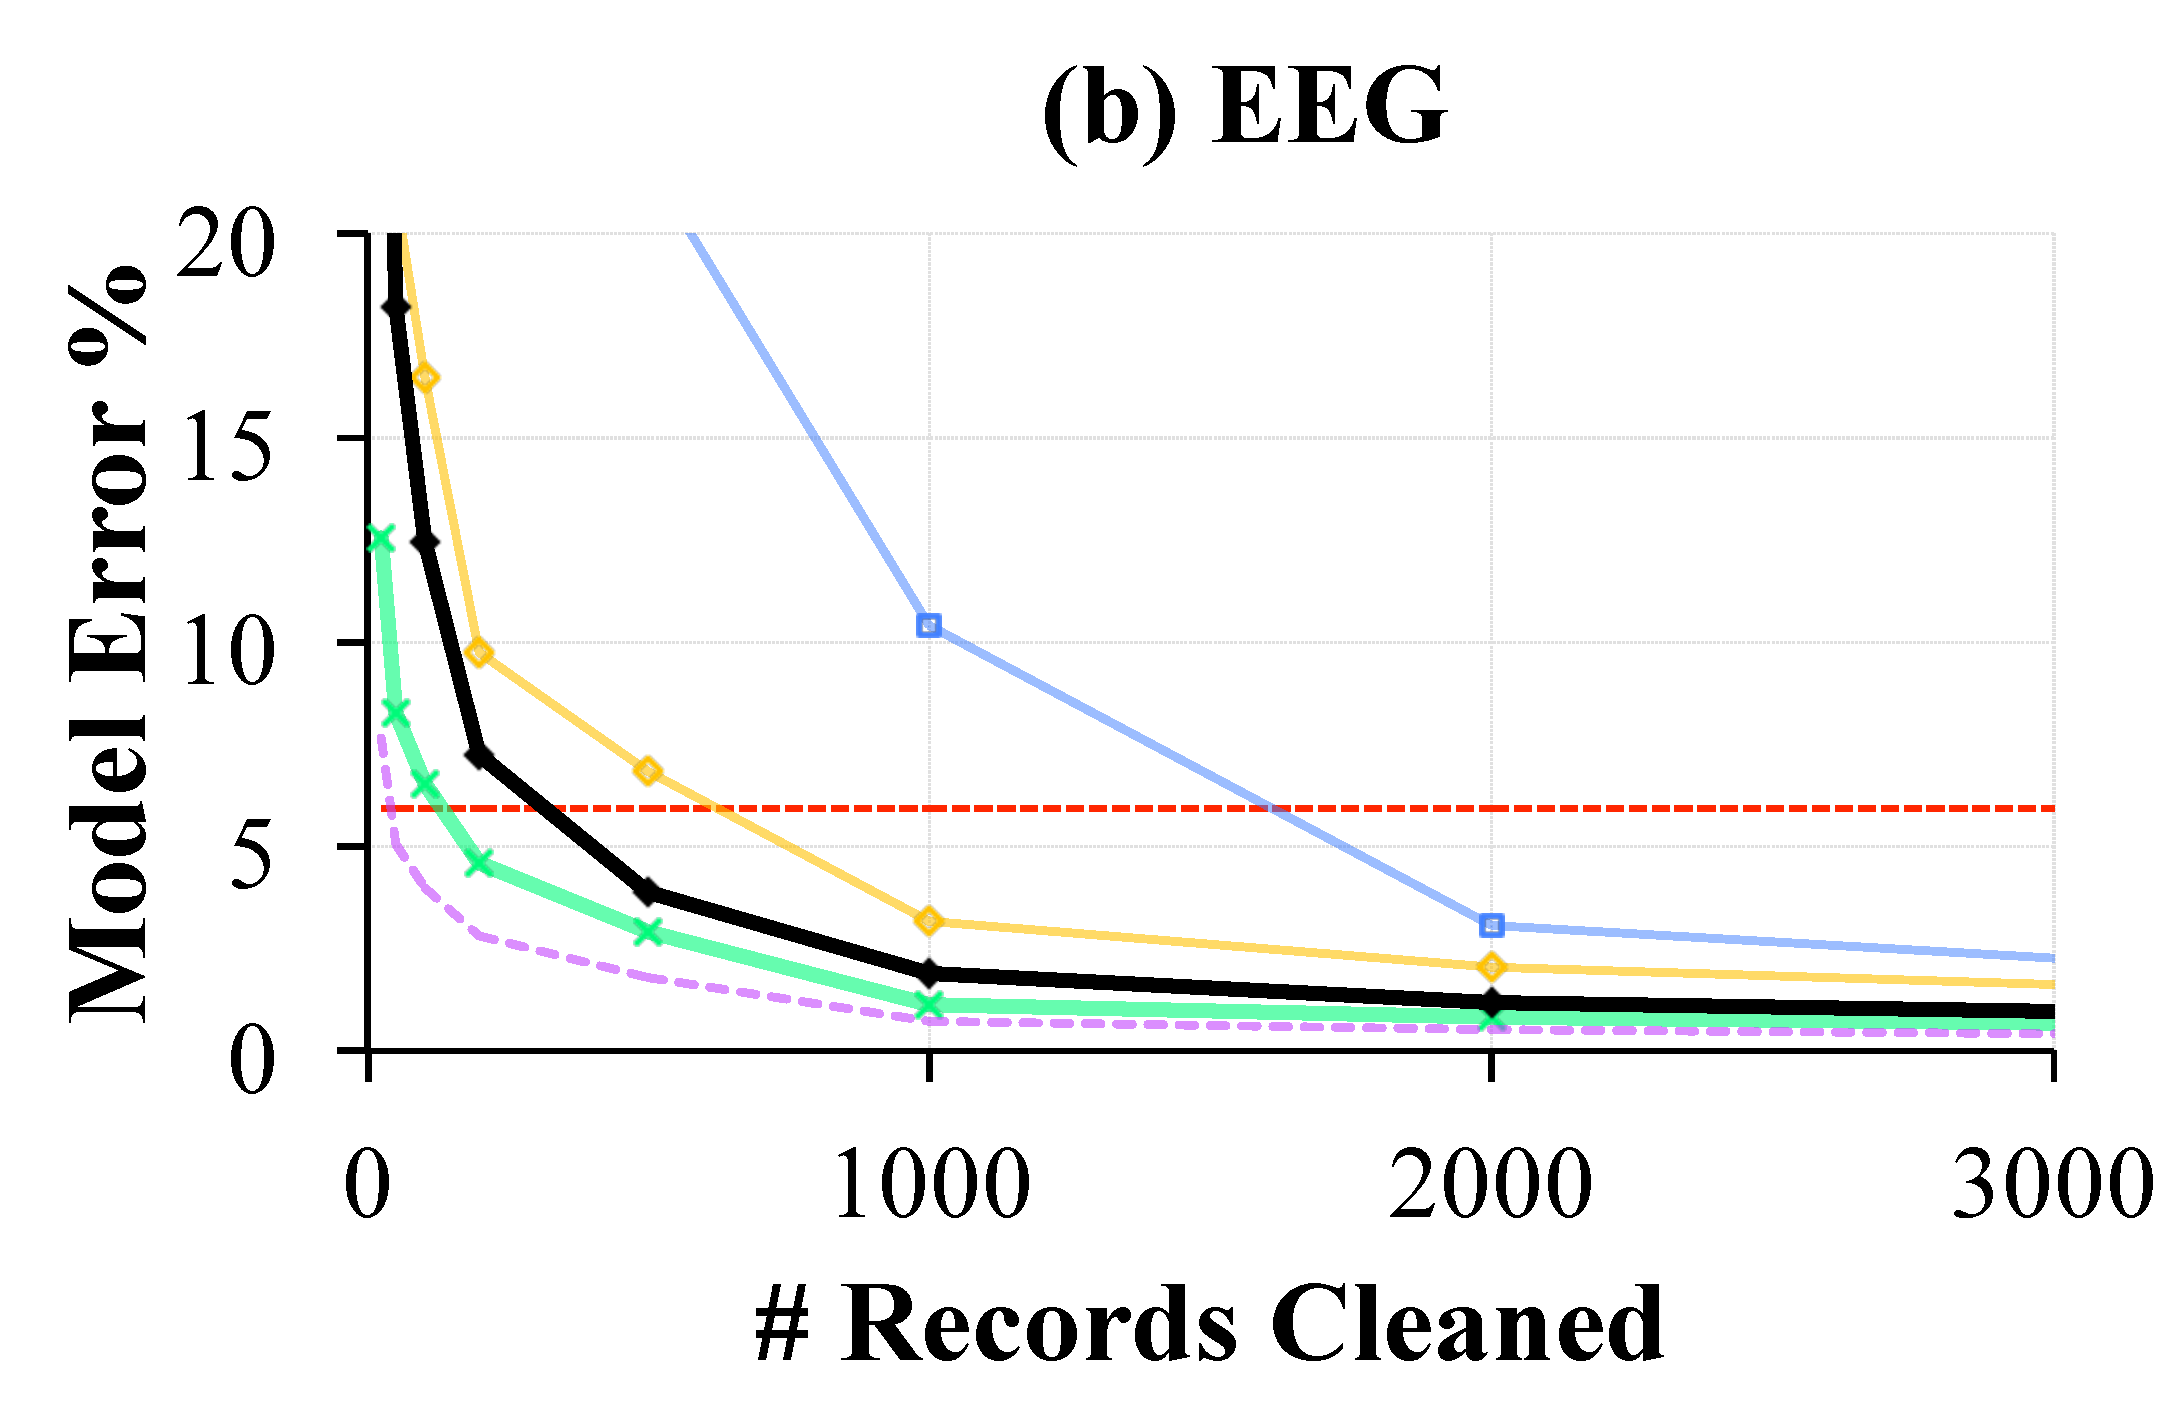
\includegraphics[width=0.49\columnwidth]{exp/exp11b.pdf}
 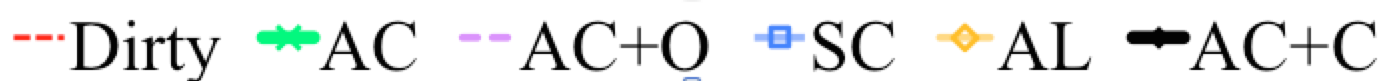
\includegraphics[width=0.49\columnwidth]{exp/legend-11.png}\vspace{-0.5em}
 \caption{Even with a classifier \sys converges faster than Active Learning and SampleClean. \label{pred-perf}}\vspace{-1.0em}
\end{figure}


\subsubsection{Classifiable Errors}
The adaptive case depends on being able to predict corrupted records.
For example, random corruption not correlated with any other data features may be hard to learn.
As corruption becomes more random, the classifier becomes increasingly erroneous.
The next experiment explores making the systematic corruption more random.
Instead of selecting the highest valued records for the most valuable features, we corrupt random records with probability $p$. 
We compare these results to AC-D where we do not have a detector at all at one vertical slice of the previous plot (cleaning 1000 records).
Figure \ref{tradeoffs2}a plots the relative error reduction using a classifier.
When the corruption is about 50\% random then there is a break even point where no detection is better.
This is because the classifier is imperfect and misclassifies some data points incorrectly as cleaned.

\vspace{0.25em}

\noindent \emph{Summary: When errors are increasingly random (50\% random) and cannot be accurately classified, adaptive detection provides no benefit over no detection. }

\begin{figure}[ht!]
\centering \vspace{-1em}
 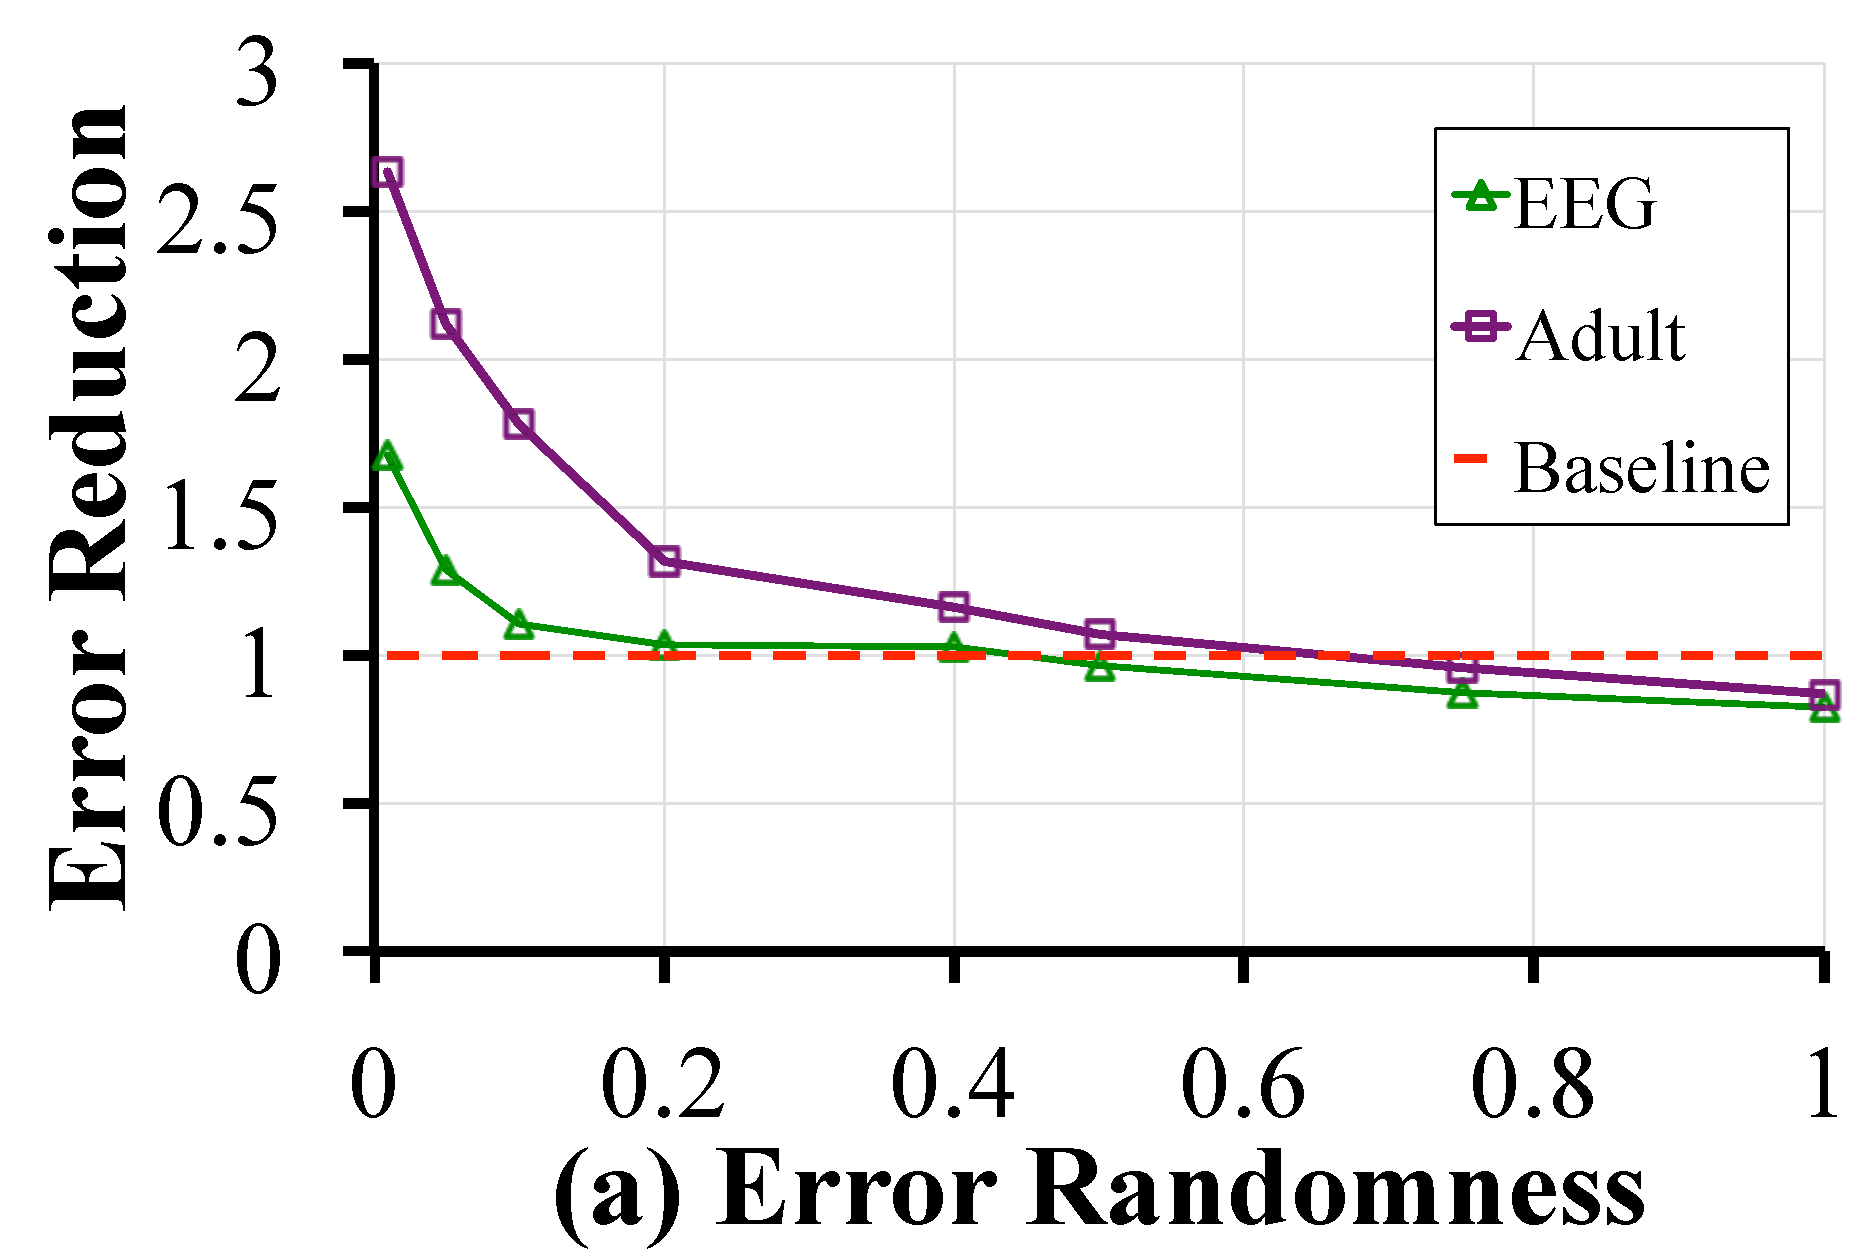
\includegraphics[width=0.49\columnwidth]{exp/exp5a.pdf}
 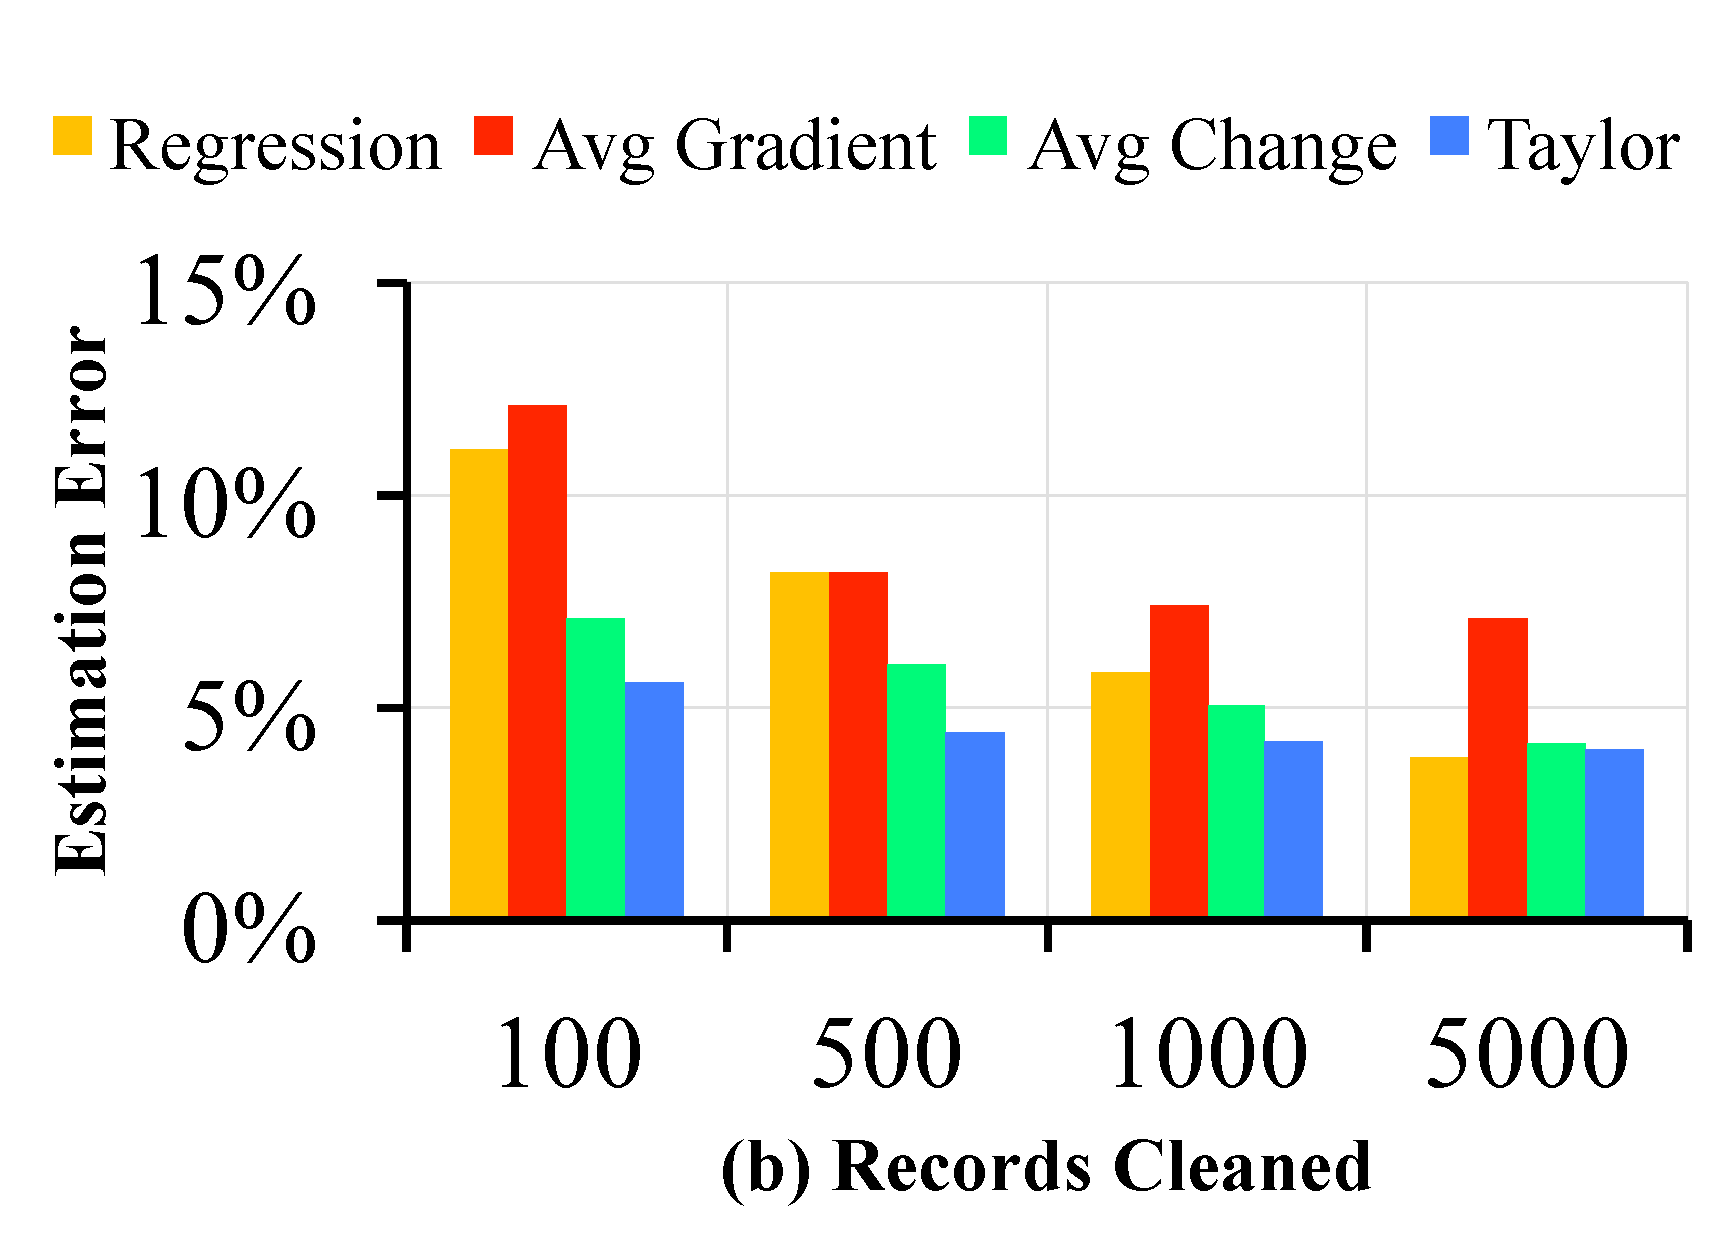
\includegraphics[width=0.49\columnwidth]{exp/exp12.pdf}\vspace{-0.5em}
 \caption{(a) Data corruptions that are less random are easier to classify, and lead to more significant reductions in relative model error. (b) The Taylor series approximation gives more accurate estimates when the amount of cleaned data is small. \label{tradeoffs2}}\vspace{-2em}
\end{figure}

\vspace{1.5em}
\subsection{Estimation}\label{est}
The next experiment compares estimation techniques: (1) ``linear regression" trains a linear regression model that predicts the clean gradient as a function of the dirty gradient, (2) ``average gradient" which does not use the detection to inform how to apply the estimate, (3) ``average feature change" uses detection but no linearization, and (4) the Taylor series linear approximation.
Figure \ref{tradeoffs2}b measures how accurately each estimation technique estimates the gradient as a function of the number of cleaned records on the EEG dataset.

Estimation error is measured using the relative L2 error with the true gradient.
The Taylor series approximation proposed gives more accurate for small cleaning sizes, confirming the analysis in Section \ref{acc}.
Linear regression and the average feature change technique do eventually perform comparably but only after cleaning much more data.

\vspace{0.25em}

\noindent \emph{Summary: Linearized gradient estimates are more accurate when estimated from small samples. }

\subsection{Real World Scenarios}
The next set of experiments evaluate \sys in two real world scenarios, one demonstrating the \emph{a priori} case and the other for the adaptive detection case.

\subsubsection{A Priori: Constraint Cleaning}\label{dfd-exp}
The first scenario explores the Dollars for Docs dataset published by ProPublica described throughout the paper.
To run this experiment, the entire dataset was cleaned up front, and simulated sampling from the dirty data and cleaning by looking up the value in the cleaned data (see Appendix \ref{dfd-errors} for constraints, errors, and cleaning methodology).
Figure \ref{dfd}a shows that \sys converges faster than Active Learning and SampleClean.
To achieve a 4\% relative error (i.e., a 75\% error reduction from the dirty model), \sys cleans 40000 fewer records than Active Learning.
Also, for 10000 records cleaned, \sys has nearly an order of magnitude smaller error than SampleClean.

Figure \ref{dfd}b shows the detection rate (fraction of disallowed research contributions identified) of the classifier as a function of the number of records cleaned. 
On the dirty data, we can only correctly classify 66\% of the suspected examples (88\% overall accuracy due to a class imbalance).
On the cleaned data, this classifier is nearly perfect with a 97\% true positive rate (98\% overall accuracy).
\sys converges to the cleaned accuracy faster than the alternatives with a classifier of 92\% true positive rate for only 10000 records cleaned.

\vspace{0.25em}

\noindent \emph{Summary: To achieve an 80\% detection rate, \sys cleans nearly 10x less records than Active Learning. }

\begin{figure}[t]
\centering\vspace{-1em}
 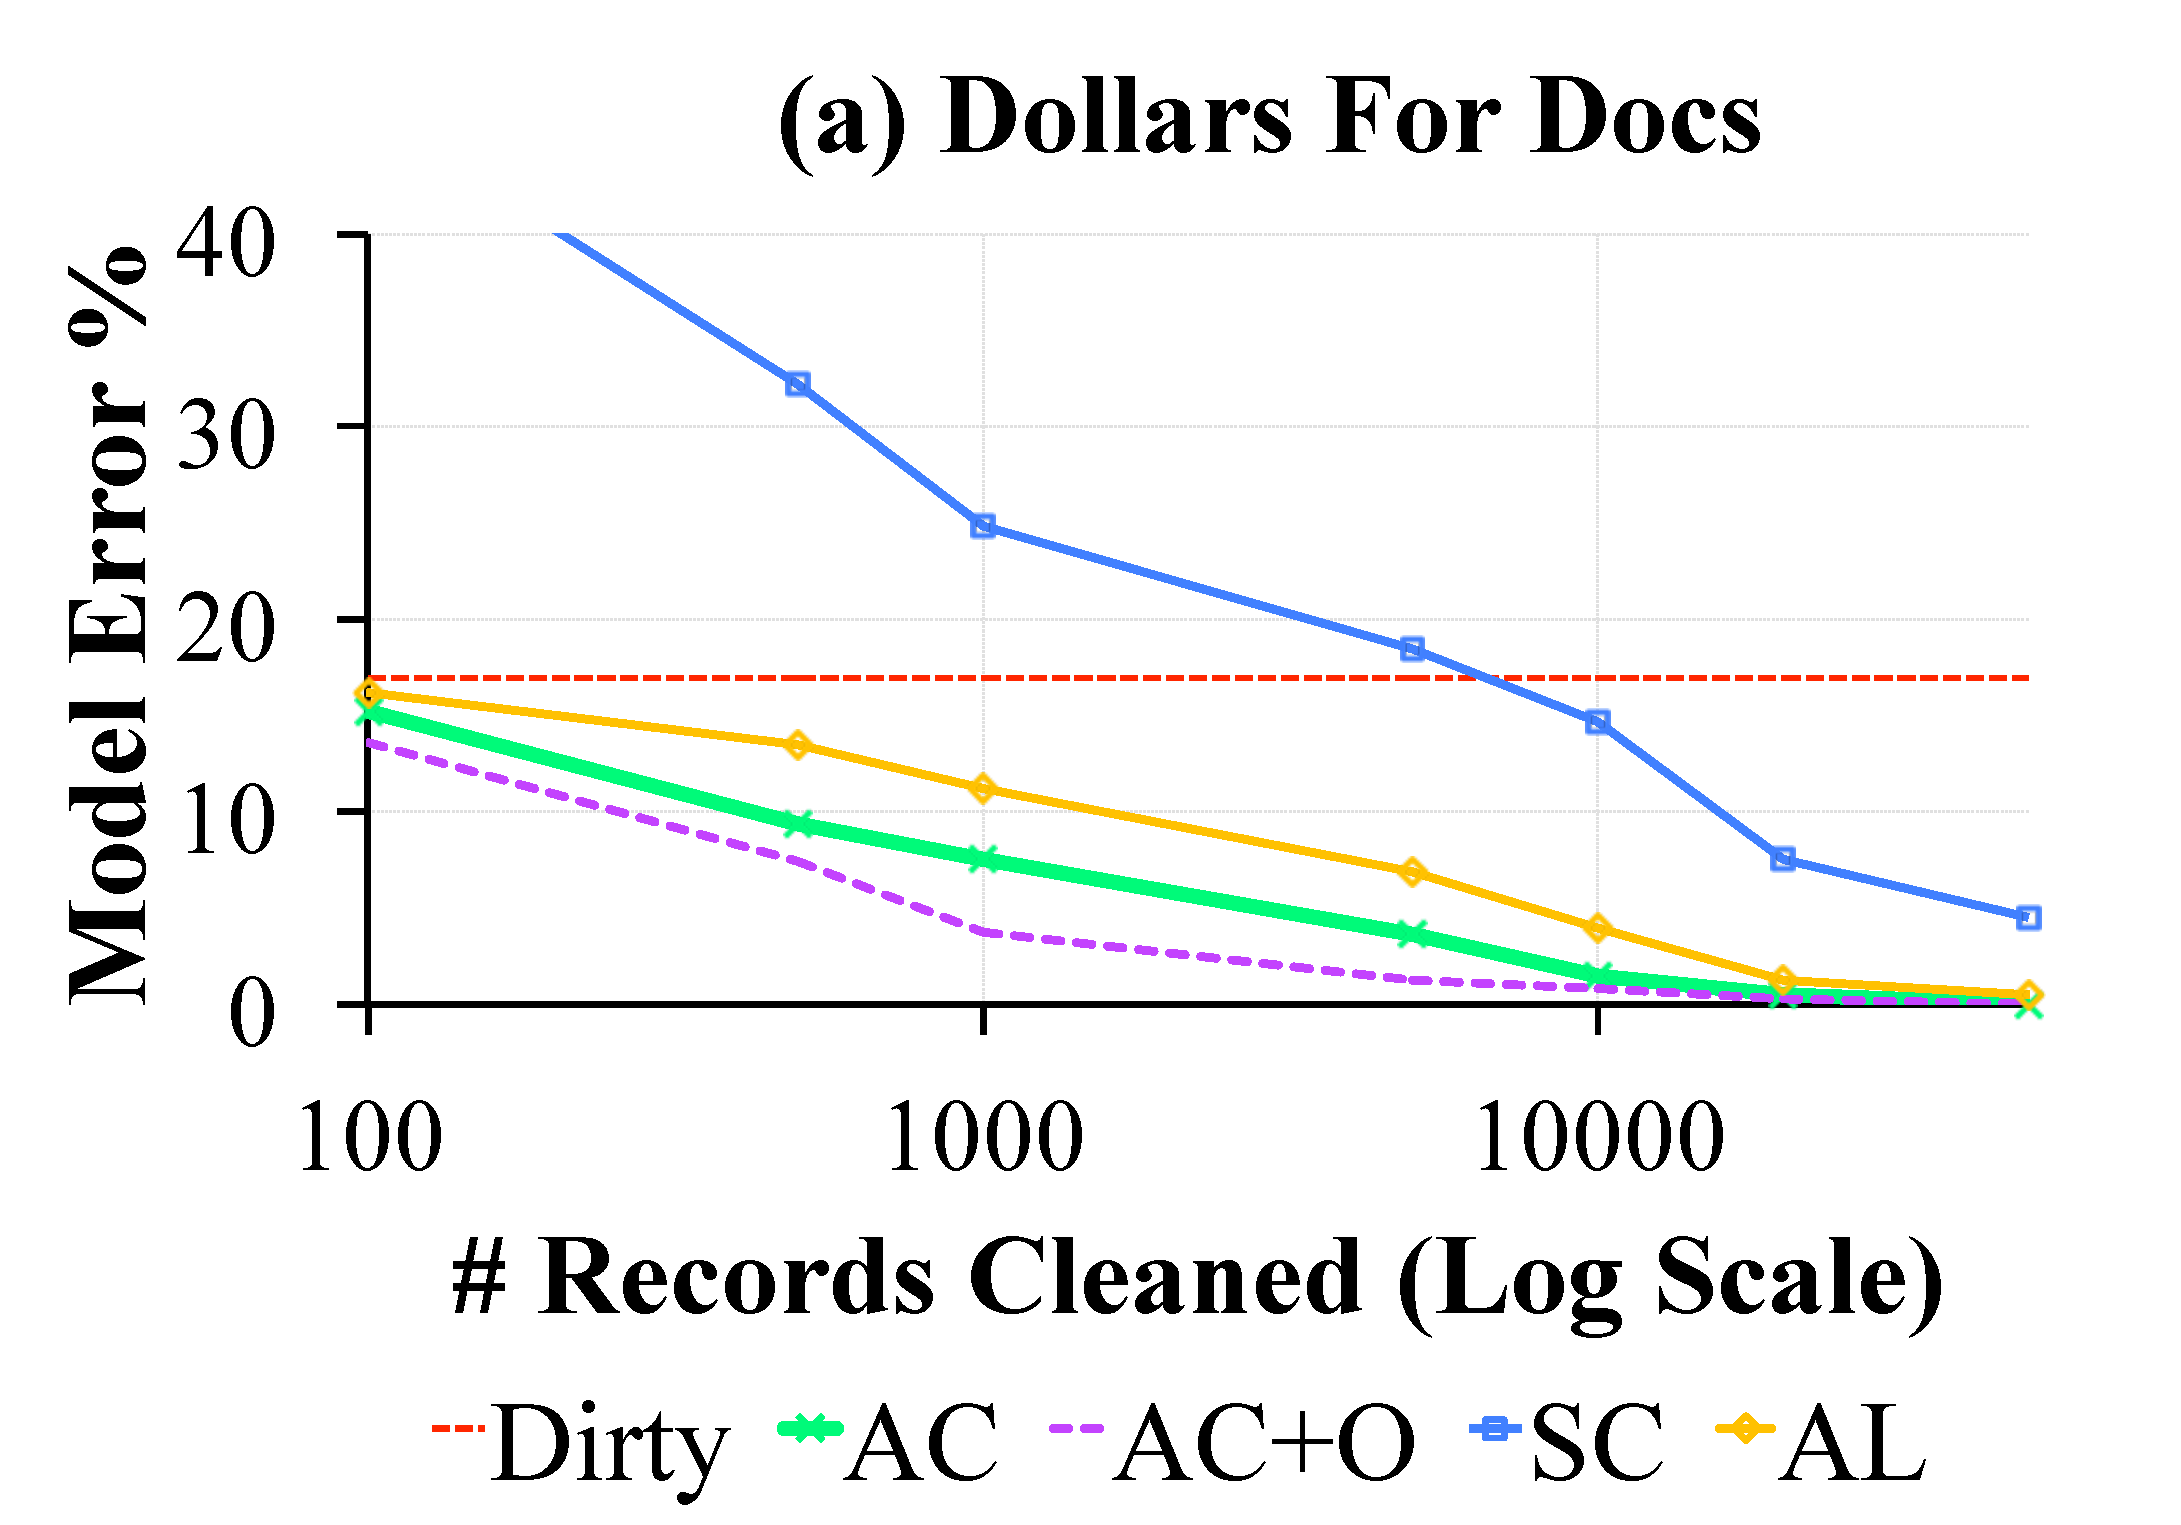
\includegraphics[width=0.49\columnwidth]{exp/exp13a.pdf}
 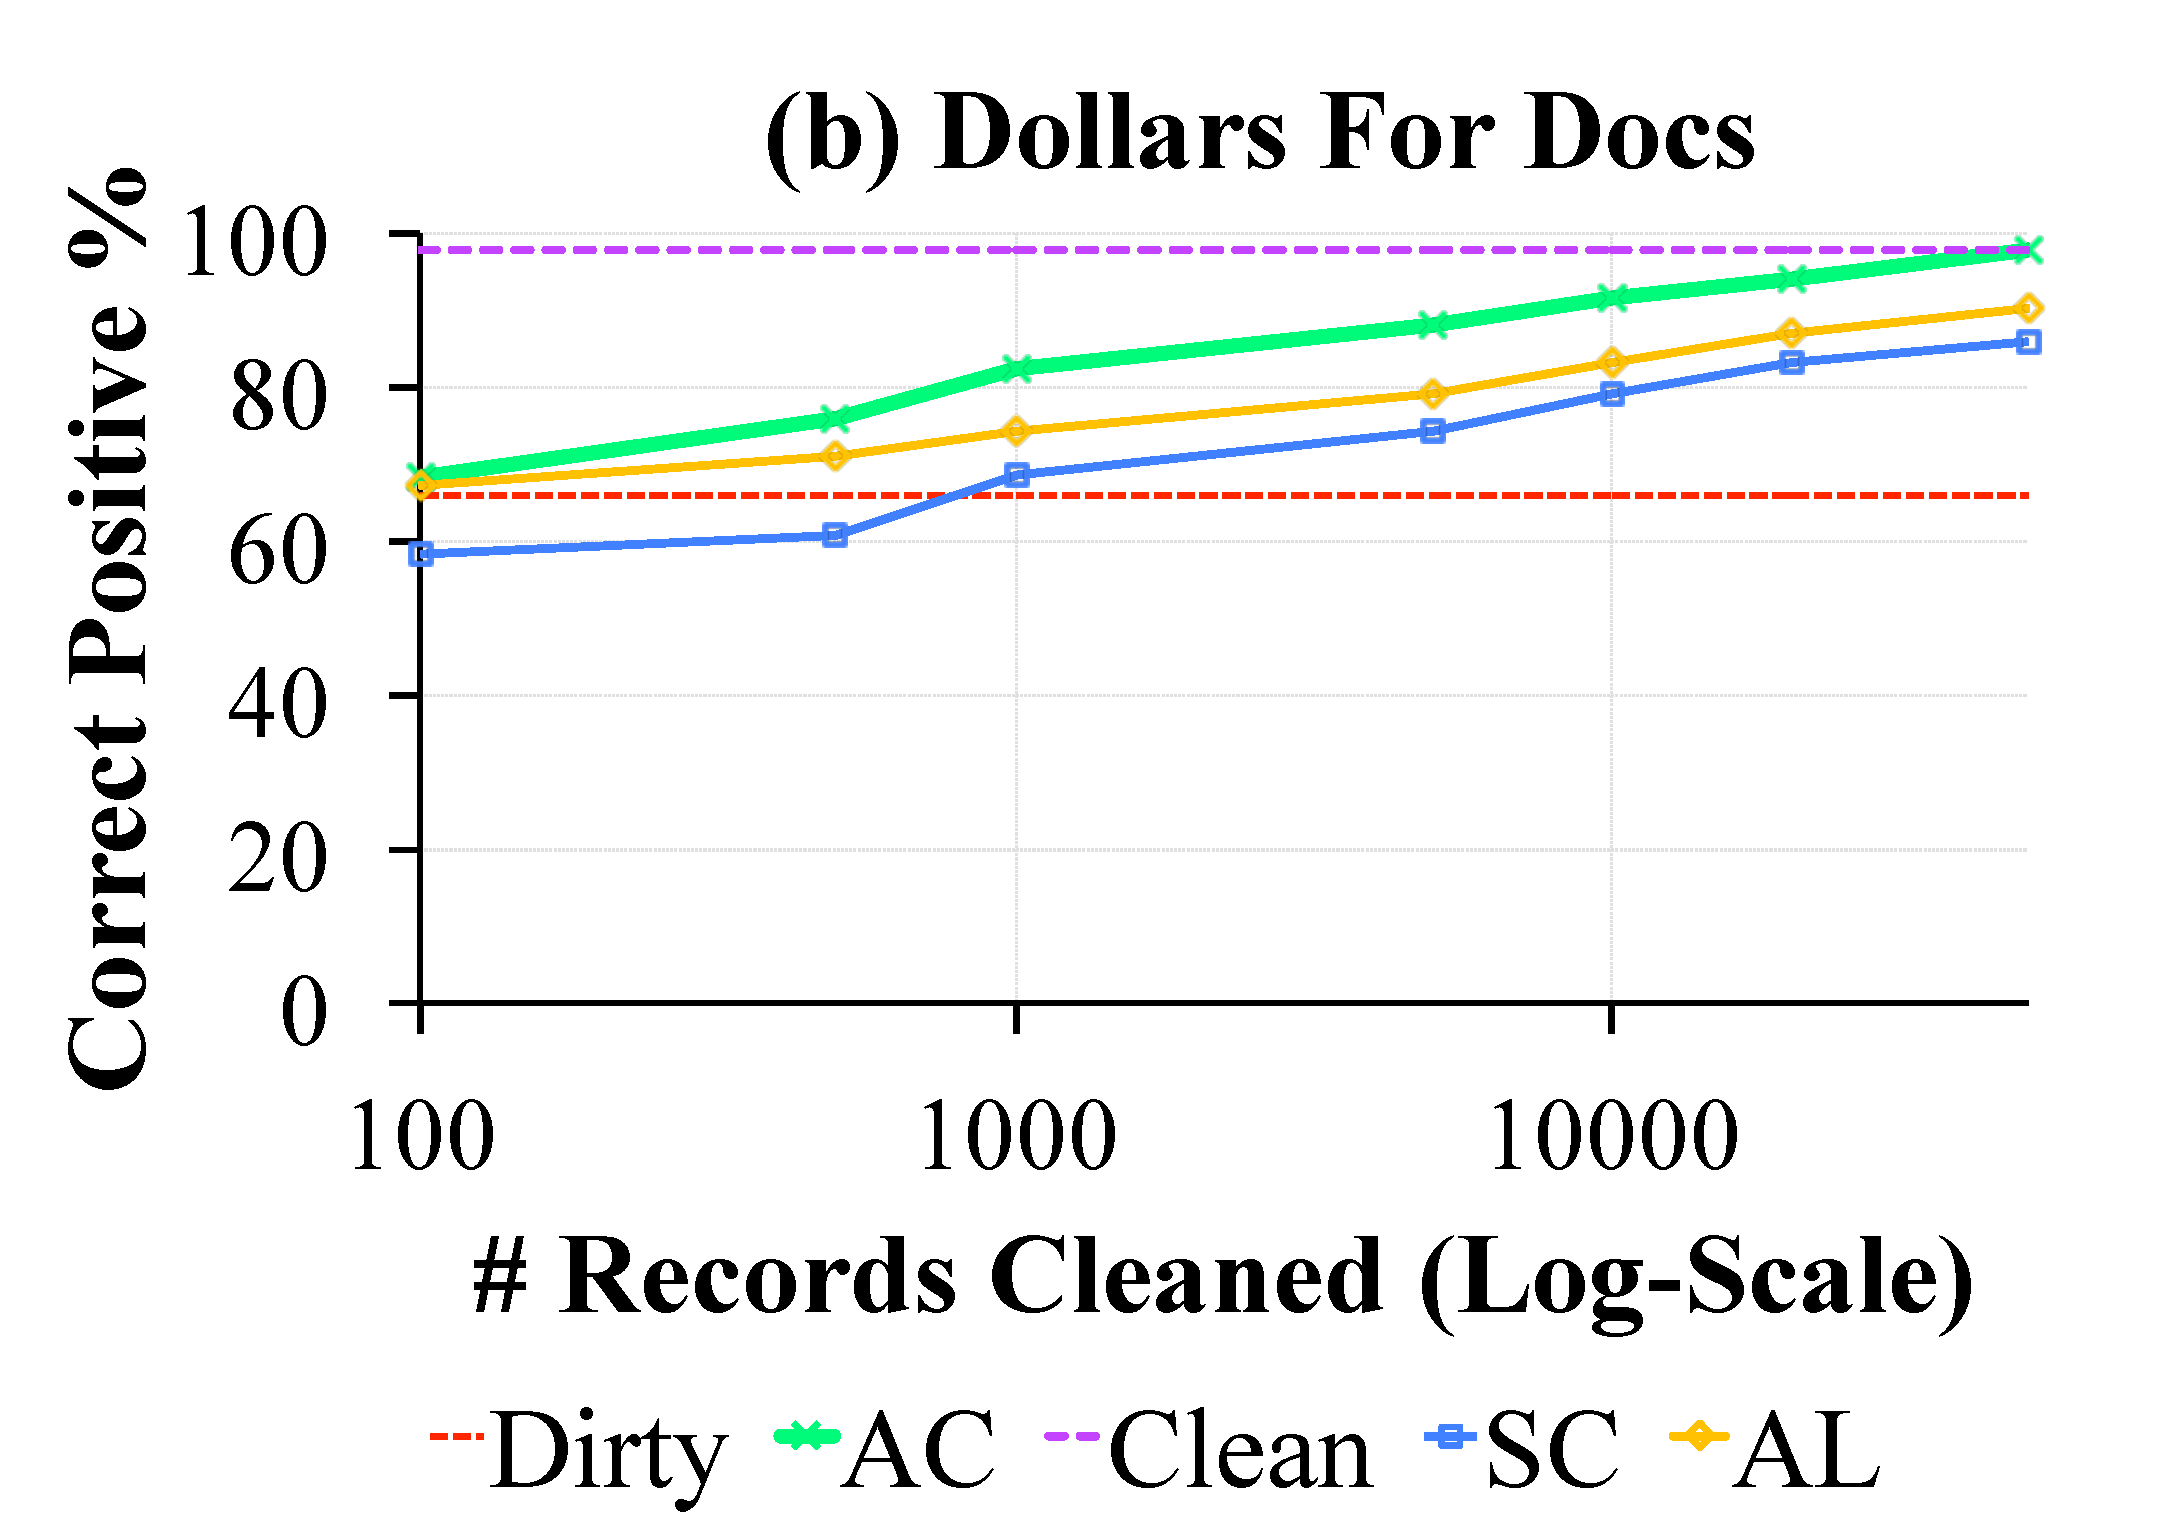
\includegraphics[width=0.49\columnwidth]{exp/exp13b.pdf}\vspace{-1em}
 \caption{(a) The relative model error as a function of the number of cleaned records. (b) The true positive rate as a function of the number of cleaned records. \label{dfd}}
\end{figure}

\subsubsection{Adaptive: Replacing Corrupted Data}
The next experiment explores the MNIST handwritten digit recognition dataset with a MATLAB image processing pipeline.
In this scenario, the analyst must inspect a potentially corrupted image and replace it with a higher quality one.
The MNIST dataset consists of 64x64 grayscale images.
There are two types of simulated corruptions: (1) 5x5 block removal where a random 5x5 block is removed from the image by setting its pixel values to 0, and (2) Fuzzy where a 4x4 moving average patch is applied over the entire image.
These corruptions are applied to a random 5\% of the images, and mimic the random (Fuzzy) vs. systematic corruption (5x5 removal) studied in the previous experiments.
The adaptive detector uses a 10 class classifier (one for each digit) to detect the corruption.

Figure \ref{mnist} shows that \sys makes more progress towards the clean model with a smaller number of examples cleaned.
To achieve a 2\% error for the block removal, \sys can inspect 2200 fewer images than Active Learning and 2750 fewer images than SampleClean.
For the fuzzy images, both Active Learning and \sys reach 2\% error after cleaning fewer than 100 images, while SampleClean requires 1750.

\vspace{0.25em}

\noindent \emph{Summary: In the MNIST dataset, \sys significantly reduces (more than 2x) the number of images to clean to train a model with 2\% error. }

\begin{figure}[t]
\centering
 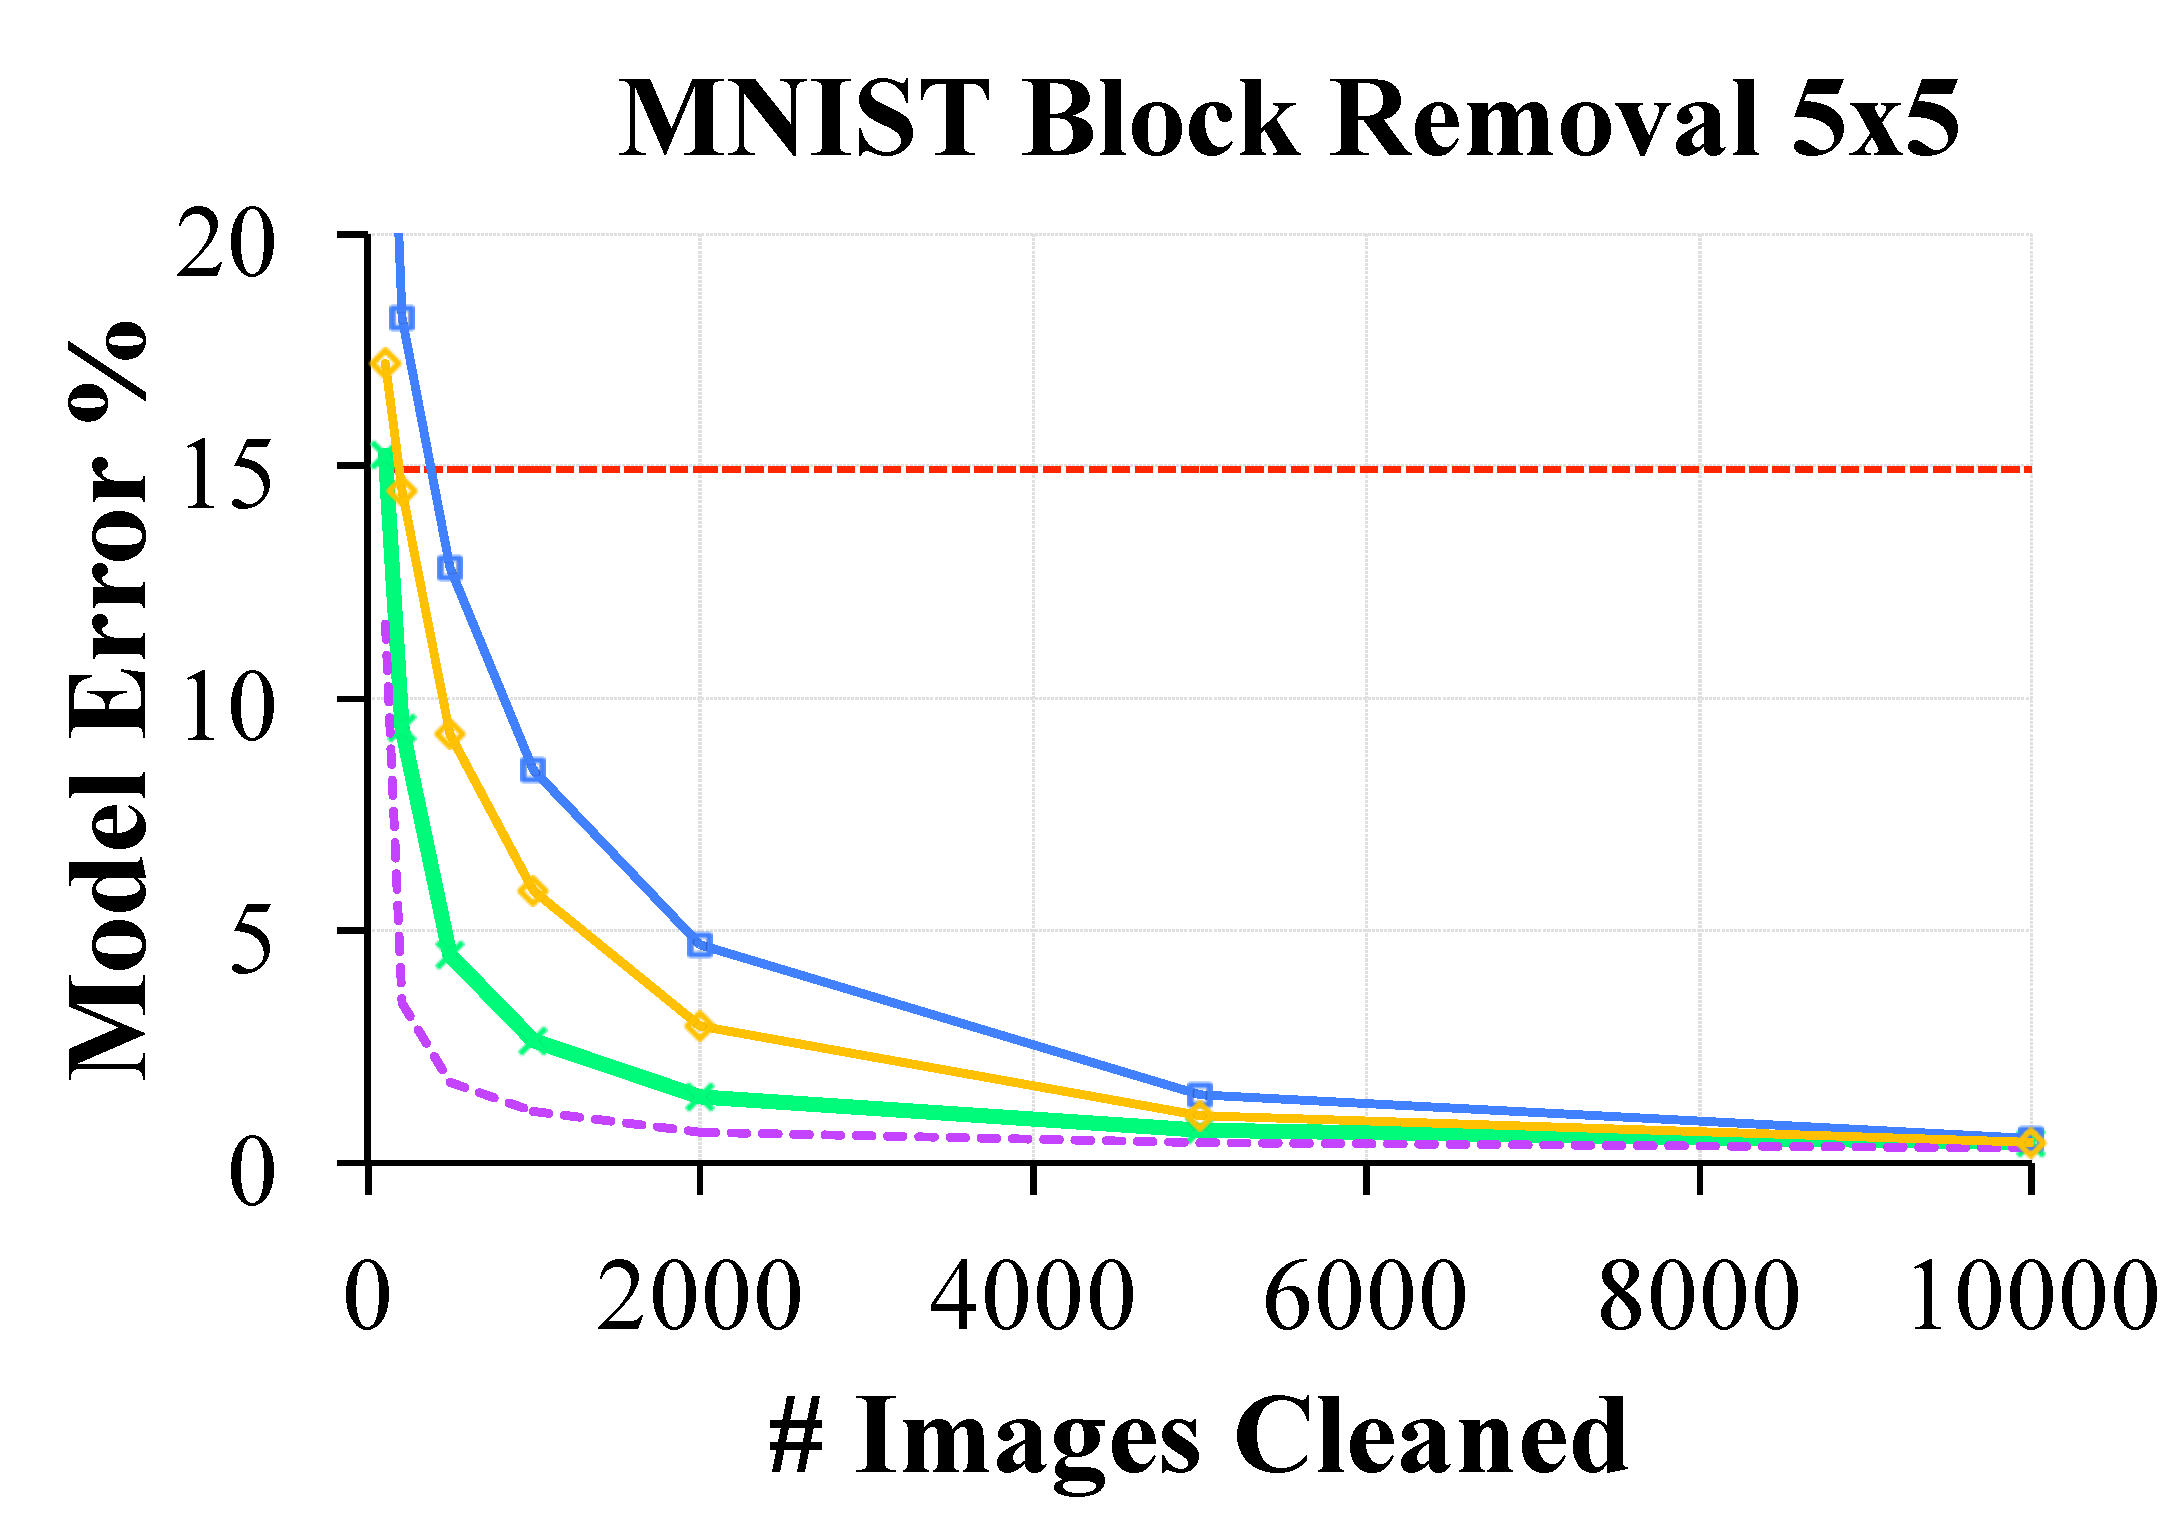
\includegraphics[width=0.49\columnwidth]{exp/exp7a.pdf}
 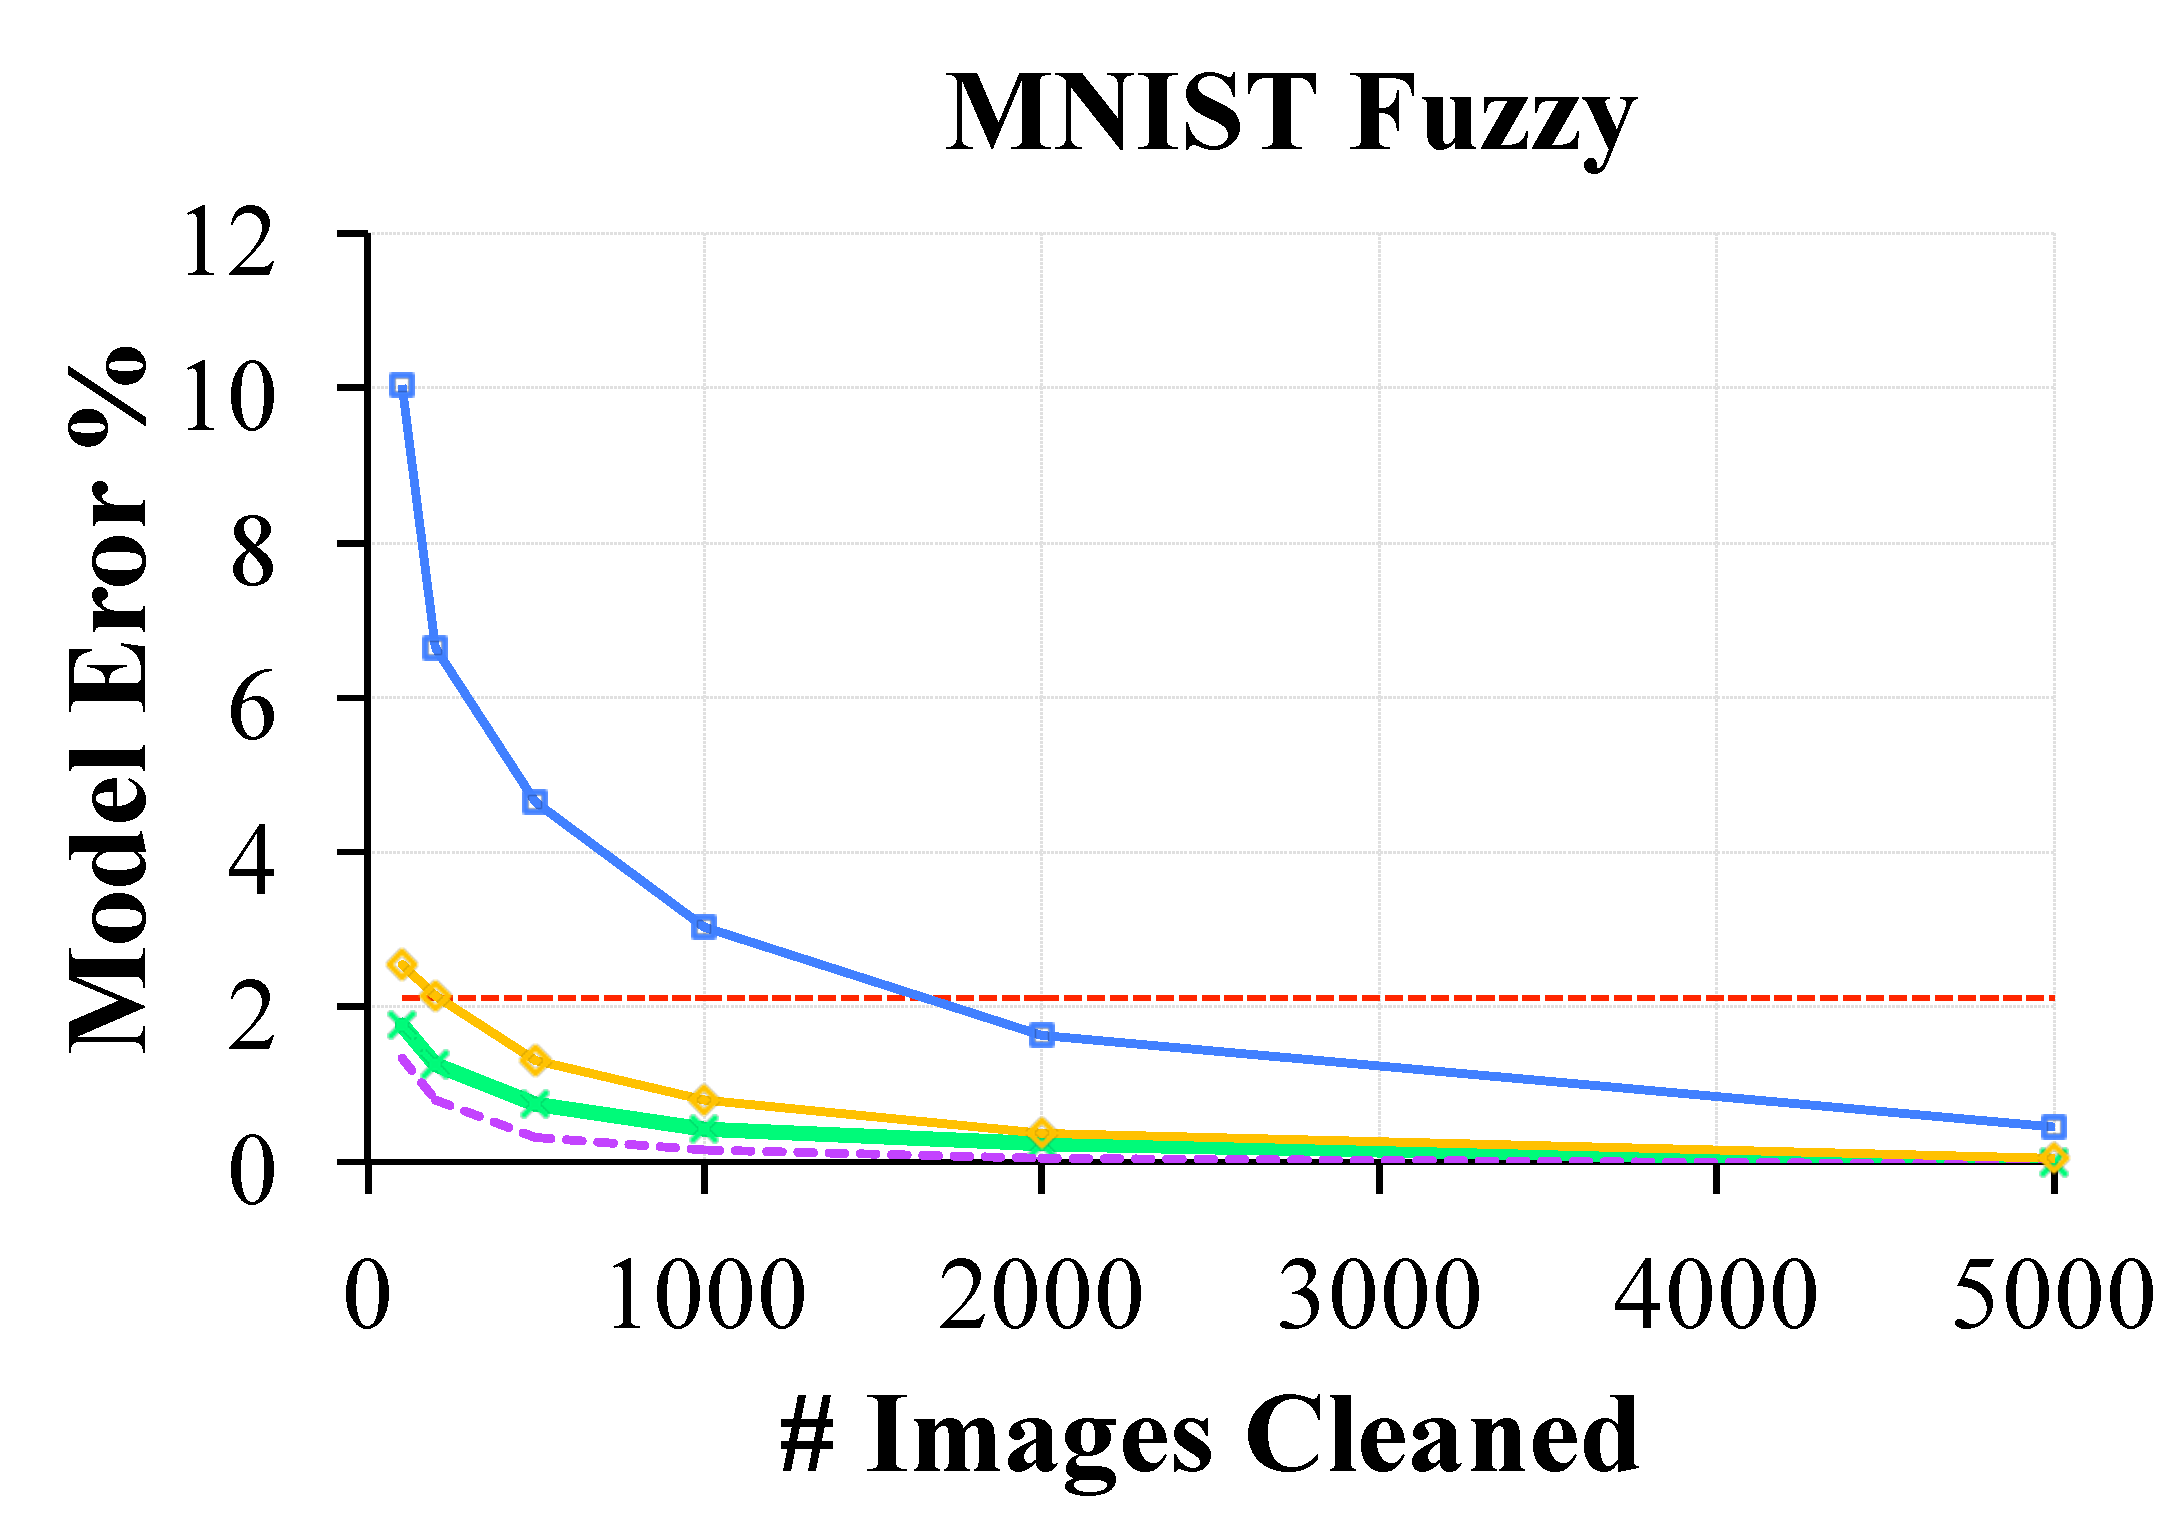
\includegraphics[width=0.49\columnwidth]{exp/exp7b.pdf}
 
\includegraphics[width=0.49\columnwidth]{exp/legend-general.png}\vspace{-0.5em}
 \caption{In a real adaptive detection scenario with the MNIST dataset, \sys outperforms Active Learning and SampleClean.  \label{mnist}}\vspace{-1em}
\end{figure}

\vspace{-.5em}
\section{Conclusion and Future Work}\label{sec:con}
In this paper, we explore using sampling, integrated with data cleaning, to improve answer quality. We propose \saqpplus, a novel framework which only requires users to clean a sample of data, and utilizes the cleaned sample to obtain unbiased query results with confidence intervals.
We identify three types of data errors (i.e., value error, condition error and duplication error) that may affect query results, and develop \biascorrected and \sampleclean to estimate query results for the data with these errors.
Our analysis and experiments suggest that \saqpplus, which returns the better result between \biascorrected and \sampleclean, is robust to different magnitudes and rates of data errors, and consistently reports good estimate results.
%Moreover, \saqpplus can optimally satisfy user-specified cleaning-cost or result-quality constraints.
Our experiments on both real and synthetic data sets indicate that \saqpplus only needs to clean a small sample of the data to achieve accurate results, and furthermore the size of this sample is independent of the size of the dataset.
In particular, \sampleclean, which processes queries only on the cleaned sample, not only makes the query processing more scalable, but surprisingly may provide higher quality results than an aggregation of the entire dirty data (\alldirty).

To the best of our knowledge, this is the first work to marry data cleaning with sampling-based query processing.
%But, it is merely the tip of the iceberg.
There are many research directions for future exploration. 

\vspace{.25em}
{\noindent \bf Constrained Queries:} Now that we have quantified a tradeoff between cleaning costs and result quality, we can explore query results where users can specify a cost or quality constraint. For example, users may want to know that given a cleaning budget, what is the best result quality they can achieve? Or, given a quality constraint, how many samples they need clean to meet the constraint? 
In these constrained queries, we aim to answer with an optimal cost or most accurate result to meet the constraints.

\vspace{.25em}
{\noindent \bf Uncertain Cleaning Results:}  Our framework can return unbiased query results with respect to AllClean for a variety of different data cleaning approaches.
We are also interested in how we can incorporate uncertain or probabilistic cleaning processes into this framework.
For example, given a dirty record, could the data cleaning module specify a set of ranges for each attribute? 
We are interested in what guarantees, if any, we can achieve in such settings.

\vspace{.25em}
{\noindent \bf Complex SQL Queries:} Another important avenue of future work is to extend our framework to support more complex SQL queries such as join and nested SQL queries. There are some straightforward methods to implement these queries. For example, we can materialize the join result as a single table, and then apply our framework to the materialized table. But this could be very costly for large datasets, thus we need to explore more efficient implementations.
For a larger set of queries, it may not be possible to estimate their results with the CLT.
Thus, exploring empirical estimation approaches (such as bootstrapping) to our framework is another interesting future direction.

\vspace{.25em}
{\noindent \bf Sample Maintenance:} Finally, in real applications users may create multiple samples from the data.
Maintaining these samples for data updates is also very challenging and needs to be investigated.


\vspace{1.5em}

\fussy
{\noindent  \bf Acknowledgements.} {\small  The authors would like to thank Sameer Agarwal, Bill Zhao, and the SIGMOD reviewers for their insightful feedback. This research is supported in part by NSF CISE Expeditions Award CCF-1139158, LBNL Award 7076018, DARPA XData Award FA8750-12-2-0331, the European Research Council under the FP7, ERC MoDaS, agreement 291071, and by the Israel Ministry of Science, and gifts from Amazon Web Services, Google, SAP, The Thomas and Stacey Siebel Foundation, Apple, Inc., Cisco, Cloudera, EMC, Ericsson, Facebook, GameOnTalis, Guavus, Hortonworks, Huawei, Intel, Microsoft, NetApp, Pivotal, Samsung, Splunk, Virdata, VMware, WANdisco and Yahoo!.
}
\sloppy



\vspace{-1em}

\bibliographystyle{abbrv}
%\scriptsize
\fontsize{8.00pt}{8.5pt} \selectfont
\bibliographystyle{abbrv}
\bibliography{ref} 

%\clearpage
\newpage
\section{Appendix}
The appendix is organized in the following way.
In Section \ref{app:proof}, we prove the unbiasedness of our estimation.
In Section \ref{app:ext}, we discuss how \sampleclean and \bias can be extended to different functions, including \varfunc.
Finally in Section \ref{app:ext2}, we discuss how \bias can be extended to make unbiased estimates from existing sample aggregations.

\subsection{Proofs}\label{app:proof}
In this section, we detail the theorems and the lemmas used in the paper.
Our main goal is to show that our estimates are unbiased; that is in expectation (denoted by $\mathbb{E(.)}$) they give the right answer.
Throughout these proofs, we will apply some key properties of expected values, for random variables $x$ and $y$:
\begin{itemize}
\item Linearity: $\mathbb{E}(ax+by)=a\mathbb{E}(x)+b\mathbb{E}(y)$
\item Independence: if $x$ and $y$ are independent then \\$\mathbb{E}(f(x)g(y))=\mathbb{E}(f(x))\mathbb{E}(g(y))$
\item Measurable functions: $\mathbb{E}(f(x))= \int f(x) \mathbb{P}(x)$ or in the discrete case $\mathbb{E}(f(x))= \sum f(x) \mathbb{P}(x)$
\end{itemize}

\subsubsection{Unbiased Estimates From Reweighted Data}
We proposed a reweighting technique to account for the over-representation of duplicates in samples.
To show that this gives us an unbiased estimate, our proof strategy will be to prove results on the full dataset, and then extend the results to a sample.

{\noindent \bf \avgfunc query:}
We begin with the following basic lemma about reweighting the entire dataset and how a mean of the reweighted data differs from the true mean.

\setcounter{lemma}{0}
\begin{lemma}
Let $P$ be a population with $N$ data tuples, and $P_{u}$ be the cleaned population with $N'$ unique data tuples.
For each $p_{i}\in P$, let $m_i$ denote the number of its duplicates in $P$.
Then mean value of the set $\saqpplusfunc(P)=\{\frac{p_{1}}{m_{1}},\frac{p_{2}}{m_{2}},...,\frac{p_{N}}{m_{N}}\}$ is:
\[
mean(\frac{N}{N'}\saqpplusfunc(P))= mean(\hat{P}_{u})
\]
\end{lemma}

Proof: The function $\saqpplusfunc$ acts point-wise on the elements of the dirty set $P$, creating a new set $\saqpplusfunc(P)$.
Therefore:
\[
mean(\saqpplusfunc(P)) = \frac{1}{N}\sum_i^N \frac{x_i}{m_i}
\]
We collect all the terms with the same value; that is a set ${i:x_i=z}$.
We call the set of distinct values the support, denoted by $supp(p)$.
\[
mean(\saqpplusfunc(P)) = \frac{1}{N}\sum_{z \in supp(p)} z(\sum_i \frac{1}{m_i})
\]
If we mutliply each $z$ by $\frac{N'}{N}$, then:
\[
mean(\saqpplusfunc(P)) = \sum_{z \in supp(p)} z\frac{(\sum_i \frac{1}{m_i})}{N'}
\]

The aggregation attributes of a population of numerical tuples can be interpreted as a discrete probability distribution.
For example, in the set $\{1, 1, 3\}$, we can say that an equivalent representation is a distribution $p(x)$, where $p(1)=\frac{2}{3}$,
and $p(3)=\frac{1}{3}$.
This probability distribution is exactly the probablity that a value will be drawn in a uniform random sampling.
Furthermore, let us say that $p(x)$ is a representation for the clean population $P_{u}$.
The expected value of this distribution is consistent with the mean of the set:
\[
\mathbb{E}(p(x)) = \sum_z z \mathbb{P}(x=z)
\]
\[
\mathbb{E}(p(x)) = mean(P_{u})
\]
and furthermore $\mathbb{P}(x=z)=\frac{(\sum_i \frac{1}{m_i})}{N'}$:
\[
mean(\frac{N}{N'}\saqpplusfunc(P))= mean(\hat{P}_{u})\blacksquare
\]

We use this lemma to prove that our estimates on a sample are unbiased.
This was presented as Lemma \ref{lem:derror} in paper.
Specifically, we mean that in expectation the mean of $\saqpplusfunc(S)$ is equal to result on the full cleaned data $\saqpplusfunc(P)$.
\begin{lemma}
Let $S \subseteq P$ be a sample of a population with $K$ data tuples, and $P_{u}$ be the cleaned population as defined before.
For each $s_{i}\in S$, let $m_i$ denote the number of its duplicates in $P$.
Then expected mean value of the set $\saqpplusfunc(S)=\{\frac{s_{1}}{m_{1}},\frac{s_{2}}{m_{2}},...,\frac{s_{K}}{m_{K}}\}$ is:
\[
\mathbb{E}(\frac{K}{K'}mean(\saqpplusfunc(S))) = mean(P_{u})
\]
where $K'=\sum_i\frac{1}{m_i}$.
\end{lemma}
Proof: A caveat is that $m_i$ is also a random variable.
Since, we assume uniform random sampling, we can conclude that each $s_i,m_i$ are independent from other samples:
\[
s_{i} \perp s{j}\text{, } m_{i} \perp m{j}
\]
Using this intuition, we want to isolate a sample and its duplication number.
Let us first consider a single sample $s_{i}$ from the mean calculation,
we hold out the terms relating to $i$ and express it as:
\[
\frac{K}{\frac{1}{m_i}+ \sum_{j\ne i}\frac{1}{m_j}} \frac{s_i}{m_i}
\]
With a little bit of algebraic manipulation, we can get:
\[
\frac{K(\sum_{j\ne i}\frac{1}{m_j})}{(K-1)\sum_i\frac{1}{m_i}}\cdot\frac{K-1}{\sum_{j\ne i}\frac{1}{m_j}}\cdot\frac{s_i}{m_i}
\]
Now, if we take expectations,
\[
\mathbb{E}(\frac{K(\sum_{j\ne i}\frac{1}{m_j})}{(K-1)\sum_i\frac{1}{m_i}}\frac{K-1}{\sum_{j\ne i}\frac{1}{m_j}}\frac{s_i}{m_i})
\]
apply linearity, and notice the symmetry in the problem (if we sample independently each samples is probabilistically the ``same");
we can see that by the first term will be 1 in expectation.
In other words, since we are holding out 1 item each time, which means the average will be exactly $\frac{K}{K-1}$.
We are left with:
\[
\mathbb{E}(\frac{K-1}{\sum_{j\ne i}\frac{1}{m_j}}\frac{s_i}{m_i})
\]
Applying independence to the rest of the expression, this is equal to:
\[
\mathbb{E}(\frac{K-1}{\sum_{j\ne i}\frac{1}{m_j}})\mathbb{E}(\frac{s_i}{m_i})
\]
The first term in an independent unbiased estimate of $\frac{N}{N'}$ and the second term is mean of $mean(\saqpplusfunc(P))$:
\[
\frac{N}{N'}\cdot mean(\saqpplusfunc(P)) = mean(P_{u})\blacksquare
\]

{\noindent \bf \sumfunc and \countfunc queries:}
These queries follow from the same logic as the \avgfunc query, but with a much simplified proof for both lemmas.
As we do not need to deal with a scaling factor such as $\frac{N}{N'}$, the first theorem is trivially shown by linearity of expectation.
In the second theorem, since we can treat $\frac{s_i}{m_i}$ as a single random variable (there is no dependence of $K'$ on $m_i$) so each sample
is trivially independent.
We can then use the fact that sample means are unbiased estimators of population means.

\subsubsection{Unbiased Estimates With Predicates}\label{app:proof2}
A similar proof is needed to show that estimates with predicates are unbiased.

{\noindent \bf \avgfunc queries:}
We will explore how predicates affect the \avgfunc query.
\begin{lemma}
Let $S \subseteq P$ be a sample of a population with $K$ data tuples, and $P_{1}\subset P$ be the set of tuples that satisfy the predicate.
For each $s_{j}\in S$, let $I(j)$ be an indicator function of whether the tuple satisfies the predicate or not.
Then expected mean value of the set $\saqpplusfunc(S)=\{I(1)s_1,I(2)s_2,...,I(K)s_K \}$ is:
\[
\mathbb{E}(\frac{1}{r}mean(\saqpplusfunc(S)))= mean(P_{1})
\]
where $r = \frac{\sum_j I(j)}{K}$.
\end{lemma}
Proof: We first can expand the expression, noticing that the factors of $K$ cancel out:
\[\frac{1}{r}mean(\saqpplusfunc(S)) = \frac{1}{\sum_j I(j)}\sum_n I(n)s_n \]
Since only the non-zero elements contribute to the sum, then this is the same as the mean over the elements in
the sample that satisfy the predicate.
Then, it follows that, in expectation, each sample that satisfies the predicate has mean:
\[ mean(P_{1})\]
Applying the linearity of expectation:
\[
\mathbb{E}(\frac{1}{r}mean(\saqpplusfunc(S)))= mean(P_{1})\blacksquare
\]

{\noindent \bf \sumfunc and \countfunc queries:}
Similar to duplication error, as we do not have to worry about the scaling factor $r$ for these quries the proof is greatly simplified.
In fact, as before it directly follows from the linearity of expectation.



\subsubsection{Proof of Theorem~\ref{thm:sampleclean}}\label{app:proof3}
The lemmas in the previous sections for duplication errors and predicates are careful to prove unbiased estimates only under their respective errors.
However, the theorems are general enough not to make any assumptions about the presence of other errors.
We can compose these corrections in the intuitive way; where we first set the attribute to its correct value, reweight the value by $m_i$, and set it to $0$ if it does not satisfy the predicate.

The proof is clear, since we are taking one pass making the estimate unbiased under value errors.
Then in another pass our estimate is unbiased under duplication.
Finally, we transform the set so its mean in unbiased with the predicate.

To be pedantic, the order of operations is important since our transformation sets condition errors to $0$.
Therefore, it should be the last step in the composition.
Duplication and value correction are interchangeable.

\subsubsection{Proof of Theorem~\ref{thm:bias}}\label{app:proof4}
Based on the proofs in the preceeding appendix sections, we can see how \sampleclean gives unbiased estimates.
In \sampleclean, we take a sample of data, clean it by applying the function $\saqpplusfunc$, and then aggregate the resulting set with a mean.
It directly follows from the two lemmas that for \sumfunc, \countfunc, and \avgfunc, we can achieve an unbiased estimate.
We presented this as Theorem \ref{thm:sampleclean} in the paper.

We also argued in Theorem \ref{thm:bias} that \bias gives an unbiased estimate.
The result of the aggregation function $f$ on the dirty population $P$ differs from the true result by a bias $\epsilon$:
\[f(P) = f(P_{\clean}) + \epsilon\]
We can write:
\begin{equation}
f(P) = \frac{1}{N}\sum_{t\in P}\saqpfunc(t)\hspace{2em}
f(P_{\clean}) = \frac{1}{N}\sum_{t\in P}\saqpplusfunc(t)
\end{equation}
If we solve for $\epsilon$, we find that:
\begin{equation}
\epsilon = \frac{1}{N}\sum_{t\in P}\Big(\saqpfunc(t)-\saqpplusfunc(t)\Big)
\end{equation}
In other words, for every tuple t, we calculate how much $\saqpplusfunc(t)$ changes $\saqpfunc(t)$.
For the population $P$, we can construct the set of differences between the two functions:
\[\scriptsize
Q=\{\saqpfunc(t_1)-\saqpplusfunc(t_1),\saqpfunc(t_2)-\saqpplusfunc(t_2), \cdots ,\ \saqpfunc(t_N)-\saqpplusfunc(t_N)\}
\]
The mean of this set is:
\[
\epsilon = mean(Q)
\]
Similarly, for a sample $S$, we can take a subset of $Q$:
\[\scriptsize
Q_s=\{\saqpfunc(t_1)-\saqpplusfunc(t_1),\saqpfunc(t_2)-\saqpplusfunc(t_2), \cdots ,\ \saqpfunc(t_K)-\saqpplusfunc(t_K)\}
\]
If we take the expected mean value of this set:
\[
\mathbb{E}(mean(Q_s))=\mathbb{E}(\frac{1}{K}\sum_i\saqpfunc(t_i)-\saqpplusfunc(t_i))
\]
By linearity of expectation and indpendence, we can see:
\[
\mathbb{E}(mean(Q_s))=\mathbb{E}(\saqpfunc(t_i))-\mathbb{E}(\saqpplusfunc(t_i))
\]
Using the arguments developed for sample clean:
\[
\mathbb{E}(\saqpplusfunc(t_i)) = f(P_{\clean}) 
\]
\[
\mathbb{E}(\saqpfunc(t_i)) = f(P) 
\]
Finally,
\[
\mathbb{E}(mean(Q_s))=\epsilon
\]
By linearity of expectation, if we subtract this unbiased estimate of $\epsilon$
from an existing aggregation of data, we get an unbiased estimate of $f(P_{\clean})$ $\blacksquare$.

\subsubsection{Estimate Monotonicity and Convergence}
We can also show convergence of our estimates.
\begin{theorem}
Let $r_{d}$ be the result of an aggregation of the dirty data
with an absolute error of $e_{d}$. For aggregations of the form that
we proposed, there exists a $K$ such that for all $k\ge K$ samples
cleaned the resulting estimate will always be have an error $\hat{e}(k)\le e_{d}$.
Furthermore, the sequence $\hat{e}(k),\hat{e}(k+1),....,\hat{e}(N)$
is strictly decreasing.
\end{theorem}

Proof: The proof is clear, but it is an important conceptual point
about our estimation framework. We showed in Section \ref{sec:sampleclean} that the
95\% confidence interval for \sampleclean was of the form $\pm\lambda\frac{\sigma_{c}}{\sqrt{k}}$
and \bias was of the form $\pm\lambda\frac{\sigma_{q}}{\sqrt{k}}$.
We omitted the finite population correction factor from these confidence intervals:
\[ FPC = \frac{\sqrt{N-k}}{\sqrt{N-1}}\]
So the confidence intervals should be of the form:
\[\pm FPC\lambda\frac{\sigma}{\sqrt{k}} \]
This function is strictly decreasing to 0, and therefore there exists a such that all $k\ge K$ result in an estimate bounded by the original data error.
We are not only unbiased but we are guaranteed to converge to the right result.

\subsubsection{Narrower Confidence Intervals}
The confidence intervals for the \avgfunc query presented in the paper give a conservative estimate.
This is because $r$ itself is a random variable with some additional variance.
However, our choice of $r$ leads to some cancellations actually help us get a more accurate estimate.

Consider the following analysis.
If we set the attributes that don't satisfy the predicate to $0$, it forms a mixture distribution whose variance is given by:
\[ \frac{1}{r^2}\frac{r\sigma^2+(1-r)r\mu^2}{K} \]
Or simplified:
\[\frac{\sigma^2+(1-r)\mu^2}{Kr} \]
However, in our proof, we treated $r$ as skipping the tuples do not satisfy the predicate.
If we consider the variance of the skipping interpretation, it is:
\[ \frac{\sigma^2}{rK}\]
We see that there is an additional dependence on $\mu$ in the error bars presented in the paper, but we can achieve strictly smaller error bars.

\subsection{Extensions to result estimation model}\label{app:ext}
In this section, we discuss extensions to our result estimation model.

\subsubsection{Variance and Standard Deviation}
The underlying reason why the variance function is challenging to estimate is that in general $var(X+Y) \ne var(X)+var(Y)$.
With this in mind, we will first consider the simpler case of \sampleclean.
We define the sample variance of a set of real numbers $X$ as:
\[ var(X) = \mathbb{S}(X^2)-\mathbb{S}(X)^2 \]
where $X^2$ denotes the set $X^2=\{x_1^2,x_2^2,...,x_k^2\}$, and where $\mathbb{S}(.)$ denote the sample mean of a set of numbers.
Both the quantities $\mathbb{S}(X^2)$ and $\mathbb{S}(X)^2$ can be easily estimated with our framework.
If we define a set $X^2=\{x_1^2,x_2^2,...,x_N^2\}$, we can simply apply our estimation framework to estimate a mean of that set to get $\mathbb{S}(X^2)$.
Similarly, we can simply square estimate the mean of $X$ to get $\mathbb{S}(X)^2$.
Subtracting the two values gives us an unbiased result\footnote{We omit a correction factor of $\frac{N}{N-1}$ which makes the sample variance an unbiased estimate of the population variance.}.

The problem is that while we have computed a result that is correct in expected value, calculating a confidence interval is more challenging.
Since $\mathbb{S}(X^2)$ and $\mathbb{S}(X)^2$ are not independent estimates, we cannot simply add their confidence intervals; nor can we square the intervals in $\mathbb{S}(X)^2$.
Our solution is to use a statistical bootstrap to calculate an empirical confidence interval around the estimate.

\bias follows from the same reasoning but requires a little bit more algebraic manipulation.
As defined \bias relies on the additivity of the mean function \[mean(X-Q)=mean(X)-mean(Q)\] however, in general \[var(X-Q)\ne var(X) - var(Q)\]
Recall, that $X$ represents the set of dirty tuples $\{x_1,x_2,...,x_N\}$ and $Q$ is the set of
differences between the dirty and clean data: \\$\{\saqpfunc(x_1)-\saqpplusfunc(x_1),\saqpfunc(x_2)-\saqpplusfunc(x_2),...,\saqpfunc(x_N)-\saqpplusfunc(x_N)\}$.
It turns out that variance of $var(X-Q)$ is dependent on a more complicated expression with a cross-term $cov(X,Q)$:
\[ var(X-Q) = var(X)+var(Q)-2cov(X,Q) \]
We have to estimate two quantities $var(Q)$ and $cov(X,Q)$ which we can calculate using a similar technique as in \sampleclean:
\[ var(Q) = \mathbb{S}(Q^2)-\mathbb{S}(Q)^2 \]
\[ cov(X,Q) = \mathbb{S}(XQ)-\mathbb{S}(X)\mathbb{S}(Q) \]
Where $XQ$ denotes a point-wise multiplication of the sets $X$ and $Q$.
Our method can support such forms as $\mathbb{S}(XQ)$, by materializing a single column representing \\$XQ={x_1q_1,x_2q_2,...,x_Nq_N}$.
Similar to \sampleclean, we use a statistical bootstrap to ascertain our confidence about this estimate. 

{\noindent \bf Bootstrapping:}
Bootstrapping is a well studied field in statistics \cite{hinkley1988bootstrap}, and there are many variants of the same general principle.
If we have an aggregation function $f$ and a set $X$, we apply $f$ to re-sampled versions $X$: $\{f(X_1),f(X_2),...\}$.
We iteratively build a distribution of results and can use this to empirically figure out a confidence interval (eg. 95\% of the results lie between these estimates).
The intuition behind the method is that we are empirically evaluating the sensitivity of $f$ to sampling.
For our task, a particularly Bootstrapping variant is the Bag-of-little-Bootstraps \cite{kleiner2011scalable}, which allows for convient subsampling without replacement, but in principle we can apply any technique.

\subsubsection{Geometric Mean and Product}
Another simple extension of the framework is to calculate the multiplicative analogs of \avgfunc and \sumfunc:
\begin{itemize}\vspace{-.5em}
\item $\geomeanfunc(X) = \sqrt[N]{\prod_{i=1}^Nx_i}$
\item $\productfunc(X) = \prod_{i=1}^Nx_i$
\end{itemize}
The  are only meaningful for strictly positive values, so assuming strictly positive values we can take a log of the terms $log(gm(X))$ and $log(p(X))$, and then this
problem becomes a familiar sample mean form:
\begin{itemize}\vspace{-.5em}
\item $\log(\geomeanfunc(X)) = \frac{1}{N}{\sum_{i=1}^N\log(x_i)}$
\item $\log(\productfunc(X)) = {\sum_{i=1}^N\log(x_i)}$
\end{itemize}
We can solve this sample mean form with the methods/parameters described in the earlier sections, taking an exponential of the result and the confidence intervals at the end
when reporting the results.
An example application of this is calculating conditional probabilities in a Naive Bayes classifier \cite{jordan2002discriminative}.

\subsection{\bias for a Sample Aggregation}\label{app:ext2}
We can extend the \bias algorithm to work with aggregations of samples of the dirty data.
Naturally, this will trade-off computation time for estimate variance.
This extension affects the confidence interval in a very intuitive way.
If $S_1$ is sampled independently of $S_2$, then it follows that their estimates are independent.
The variance of two independent variables is the sum of the variances.
We can calculate the variance of the aggregation on the dirty sample, and then add it to the variance of the bias estimate $\frac{\sigma_q^2}{k}$. The following shows the details of the estimation method:

\begin{enumerate}
\item Given two random samples $S_1$ and $S_2$ and an aggregation function $f(.)$
\item Apply the $\saqpfunc(.)$ to each $s_i \in S_1$ and call the result $Q(S)=\{\saqpfunc(s_1)-\saqpplusfunc(s_1),\saqpfunc(s_2)-\saqpplusfunc(s_2),...,\saqpfunc(s_k)-\saqpplusfunc(s_k)\}$
\item Calculate the mean $\hat{\mu}_q$, and the variance $\hat{\sigma}_q$ of $Q(S_1)$.
\item Calculate the variance of the aggregation on the dirty data $\sigma_d^2=var(\saqpfunc(S_2))$ 
\item Return $(f(S_2) - \hat{\mu}_q) \pm \lambda \sqrt{\frac{\hat{\sigma}_q^2}{|S_1|} + \frac{\hat{\sigma}_d^2}{|S_2|}}$.
\end{enumerate}

This does complicate the problem of duplicate estimation, since if we cannot aggregate over the entire dataset, we cannot search over the entire dataset for duplicates.
Suppose, we were restricted to duplicate search within the sample $S_2$, then we would consistently underestimate the number of duplicates for each tuple.
We develop the following theory about estimates with imperfect duplicate counts.
Intuitively, we claim that conservative duplicate correction, that is underestimating duplicates and doing this correctly/consistently, is better than no duplicate correction.

\begin{theorem}
Define $\saqpplusfunc^{1}$ be a data transformation that only corrects for false positive errors and aggregation errors.
As it does not correct for duplication errors, there will be a bias $e$, the difference between the true result and estimate:
\[ e = |f(P_{clean})- mean(\saqpplusfunc^{1}(p))|. \]
Furthermore, let $\saqpplusfunc^{2}$ be a data transformation that corrects for all three errors but may underestimate the number of duplicates for each tuples;
that is $m'_{i}\le m_{i}$.
Finally, let $\saqpplusfunc$ the data transformation that cleans correctly for all errors.
We insist that these duplicate estimates in (2) $m_{i}'$ are consistent (ie. symmetric); if tuple i is a duplicate of tuple j, the tuple j is a duplicate of tuple i.
Let $b$ be the bias of an estimate using this transformation:
\[ b = |f(P_{clean})-d_2 \cdot mean(\saqpplusfunc^{2}(p)|. \]
Then, we have the following bounds:
\begin{equation}
0 \le b \le e
\end{equation}
Where $0\le b$ is tight when $m_i'=m_i$ and $b\le e$ is tight when $m_i=1$.
\end{theorem}

Proof: We first start by looking at \saqpplusfunc, when answering an \avgfunc query.
From the results in the previous section, we know that:
\[ f(P_{\clean}) = d \cdot mean(\saqpplusfunc(P)) \]
\[ f(P_{\clean}) = d \cdot \frac{1}{|P|} \sum_p \frac{p_i}{m_i} \]
Similarly,
\[ mean(\saqpplusfunc^{1}(p)) = \frac{1}{|P|} \sum_p p_i \]
\[ d_2 \cdot mean(\saqpplusfunc^{2}(p)) = d_2 \cdot \frac{1}{|P|} \sum_p \frac{p_i}{m_i'} \]
Therefore,
\[ e = \frac{1}{|P|} |\frac{dp_i}{m_i}-{p_i}| \]
\[ b = \frac{1}{|P|} |\frac{dp_i}{m_i}-\frac{d_2p_i}{m_i'}| \]
Collecting terms:
\[ e = \frac{1}{|P|} |(\frac{d}{m_i}-1)p_i| \]
\[ b = \frac{1}{|P|} |(\frac{d}{m_i}-\frac{d_2}{m_i'})p_i| \]
since $1 \le m_i'$ and $d \ge d_2 \ge 1$, it follows that $b \le e$.
As $\frac{d}{m_i}-\frac{d_2}{m_i'} \rightarrow 0$, then we see that the
error is lower bounded by 0.
Removing the proportionality constants, this proof can be trivially extened to \sumfunc and \countfunc $\blacksquare$.





\end{document}